\documentclass[11pt]{article}
\usepackage[left=2.5cm, right=2cm, top=2.5cm, bottom=3cm, headheight=65pt, headsep=15pt]{geometry}
\usepackage[utf8]{inputenc}
\usepackage{titlesec}
\usepackage{enumitem}
\usepackage{graphicx}
\usepackage{amsmath}
\usepackage{amsfonts}
\usepackage{amssymb}
\usepackage{fancyhdr}
\pagestyle{fancy}
\fancyhf{}
\fancyhead[L]{\includegraphics[width=18cm]{imagenes/logo.pdf}}
\renewcommand{\headrulewidth}{0pt}
\fancyfoot[C]{\thepage}
\setlength{\footskip}{15pt}
\title{Informe del Proyecto}

% Paquetes tipográficos, tablas y presentación estructurada
\usepackage[T1]{fontenc}
\usepackage{lmodern}
\usepackage[spanish,es-nodecimaldot,es-noshorthands]{babel}
\usepackage[table]{xcolor}
\usepackage{longtable,booktabs,tabularx,array,multirow}
\usepackage{float,caption}
\usepackage{url}
\usepackage{microtype}
\usepackage{etoolbox}
\usepackage[parfill]{parskip}
\setlength{\parskip}{0.55em}
\setlength{\parindent}{0pt}

% Evita que thebibliography cree una sección adicional ajena a la plantilla
\patchcmd{\thebibliography}{\section*{\refname}}{}{}{}

\definecolor{azulClaro}{HTML}{E7F0FA}
\definecolor{azulUTA}{HTML}{173A64}
\definecolor{grisClaro}{HTML}{F8FAFC}
\definecolor{linea}{HTML}{CBD5E1}
\definecolor{verdeExito}{HTML}{065F46}

\setlength{\tabcolsep}{4pt}
\renewcommand{\arraystretch}{1.2}

\newcommand{\pct}{\ensuremath{\mathrm{\char37}}}
\newcommand{\pruebaok}{\textcolor{verdeExito}{\textbf{Conforme}}}
\newcommand{\resaltar}[1]{\colorbox{azulClaro}{\strut\textbf{#1}}}

\begin{document}

\titleformat{\section}{\normalfont\Large\bfseries}{\thesection}{1em}{}
\renewcommand{\thesection}{\Roman{section}}
\begin{center}
    \textbf{\underline{\normalsize INFORME DE GUÍA PRÁCTICA}}
\end{center}

\section{PORTADA}

\begin{tabbing}
\textbf{Tema:}\hspace{1cm} \= Suavizado y reducción espacial de imágenes RGB mediante \\
\> convolución manual y saltos configurables. \\
\textbf{Carrera:}\hspace{1cm} \= Software \\
\textbf{Unidad de Organización Curricular:} \hspace{1cm} \= PROFESIONAL\\
\textbf{Nivel y Paralelo:} \> Octavo ``A''\\
\textbf{Alumnos participantes:}  \> Navarro Pazmiño Maybelline Estefanía \\
\> Paredes Medina Steven Eduardo \\
\textbf{Asignatura:} \> Inteligencia Artificial \\
\textbf{Docente:} \> Ing. Rubén Eduardo Nogales Portero, Mg.
\end{tabbing}

\section{INFORME DE GUÍA PRÁCTICA}
\titleformat{\section}{\normalfont\Large\bfseries}{\thesection}{1em}{}
\renewcommand{\thesection}{\arabic{section}}

\subsection{Objetivos}
\textbf{General:}\\
Desarrollar y evaluar un sistema integral de procesamiento digital para la reducción espacial controlada de imágenes en formato RGB mediante máscaras de convolución bidimensional normalizadas y factores de submuestreo por saltos configurables, comprobando rigurosamente la exactitud matemática de las operaciones, la consistencia de la interfaz gráfica interactiva y la fidelidad de los datos exportados.

\textbf{Específicos:}\\
\begin{itemize}[itemsep=0.2em]
\item Analizar la estructura tensorial de imágenes RGB de ocho bits por canal, implementando el relleno perimetral temporal con ceros (\textit{zero-padding}) y el cálculo formal de vecindades espaciales para máscaras de dimensión impar ($3\times3$, $5\times5$ y $7\times7$).
\item Diseñar e implementar de forma determinística la convolución espacial bidimensional manual junto con la decimación controlada por saltos horizontales y verticales independientes, contrastando los filtros de promedio, gaussianos discretos y personalizados.
\item Verificar analítica y experimentalmente la concordancia estricta entre el cálculo manual puntual y el procesamiento matricial global, evaluando la preservación cromática de canales, la mitigación del fenómeno de aliasing y la persistencia de métricas en registros CSV e imágenes PNG.
\item Evaluar el comportamiento ergonómico y funcional de la interfaz de usuario desarrollada en Tkinter, garantizando la correcta visualización de matrices de pesos de hasta $7\times7$ (49 celdas) y la reactividad de los controles en tiempo real.
\end{itemize}

\subsection{Modalidad}
\begin{tabbing}
    \hspace{1cm} \= Presencial.
\end{tabbing}

\subsection{Tiempo de duración}
\begin{tabbing}
    \hspace{1cm} \= \textbf{Presenciales:} \= 12 horas \\
    \hspace{1cm} \= \textbf{No presenciales:} \= 0 horas
\end{tabbing}

\subsection{Instrucciones}
La práctica exige la representación formal de una imagen digital a color como un tensor tridimensional perteneciente al espacio discreto $\{0,\ldots,255\}^{H\times W\times 3}$. Sobre esta estructura matricial se aplican operaciones espaciales de filtrado lineal mediante máscaras cuadradas de dimensión impar ($K\times K$). Para tratar los bordes exteriores sin perder posiciones geométricas ni alterar la alineación espacial, se prescribe la incorporación de un margen perimetral relleno de ceros de grosor $p=(K-1)/2$.

Posteriormente, se ejecuta la convolución manual bidimensional sobre cada canal de color de manera independiente. La reducción dimensional se obtiene decimiendo la cuadrícula mediante saltos o avances configurables $s_h$ (horizontal) y $s_v$ (vertical), prescindiendo estrictamente del uso de librerías automáticas de redimensionado interpolado o funciones de alto nivel que oculten el cómputo matricial.

El entorno de software debe ofrecer una visualización simultánea de tres paneles: la imagen original, la reducción directa por submuestreo sin filtrado previo (línea base con susceptibilidad a aliasing) y la reducción con suavizado espacial. Asimismo, debe incorporar una herramienta de inspección interactiva que exponga el procedimiento aritmético paso a paso para cualquier píxel seleccionado por coordenadas, y una rutina de exportación en formato PNG que preserve la matriz matemática real de salida.

\subsection{Listado de equipos, materiales y recursos}
Listado de equipos y materiales empleados en el desarrollo de la práctica:
\begin{itemize}[itemsep=0.2em]
\item Computador personal de arquitectura x86\_64 con procesador multinúcleo y sistema operativo de 64 bits.
\item Entorno de ejecución Python 3.10 o superior, complementado con el gestor de paquetes \texttt{pip}.
\item Librería NumPy para la manipulación vectorizada de arreglos multidimensionales y aritmética de punto flotante de 64 bits.
\item Librería Pillow (PIL) para la decodificación de imágenes fuente, conversión de formatos de color y exportación de archivos PNG.
\item Módulo estándar Tkinter / ttk para la construcción de la interfaz gráfica de usuario de escritorio.
\item Fotografía digital de referencia en color de dimensiones $626\times417$ píxeles (\texttt{paisaje.png}).
\end{itemize}

\textbf{TAC (Tecnologías para el Aprendizaje y Conocimiento) empleadas en la práctica:}\\
$\square$ Plataformas educativas \\
$\square$ Simuladores y laboratorios virtuales \\
$\boxtimes$ Aplicaciones educativas \\
$\boxtimes$ Recursos audiovisuales \\
$\square$ Gamificación \\
$\square$ Inteligencia Artificial \\
Otros: Entorno interactivo en Python con inspección de matrices en tiempo real y exportación de métricas.

\subsection{Actividades por desarrollar}
El plan de actividades integró fases analíticas, matemáticas y de desarrollo experimental para garantizar la consistencia entre el modelo teórico y la implementación en código.

\subsubsection{Marco teórico formal del procesamiento espacial}

\textbf{Modelo matemático de la imagen digital y espacios cromáticos}

Una escena óptica continua proyectada sobre el plano focal de un sensor se modela analíticamente como una función de radiancia $f(x, y, \lambda)$, dependiente de las coordenadas bidimensionales espaciales $(x, y) \in \mathbb{R}^2$ y de la longitud de onda de radiación electromagnética $\lambda$. En sistemas de captura tricromáticos estandarizados bajo el modelo CIE 1931, la información continua se proyecta sobre tres funciones de sensibilidad espectral asociadas a los conos retinianos humanos:
\begin{equation}
C_c(x, y) = \int_{\Lambda} f(x, y, \lambda) \, s_c(\lambda) \, d\lambda, \quad c \in \{R, G, B\},
\end{equation}
donde $\Lambda$ delimita el espectro visible ($380\,\text{nm} \le \lambda \le 780\,\text{nm}$) y $s_c(\lambda)$ representa la curva espectral normalizada del canal correspondiente.

En la etapa de digitalización, este continuo se discretiza espacialmente mediante un muestreo periódico en rejilla rectangular con pasos de muestreo $\Delta x$ y $\Delta y$, y se cuantiza uniformemente en un rango discreto de intensidades enteras:
\begin{equation}
I[y, x, c] = \mathcal{Q}\Big( C_c(x \cdot \Delta x, \; y \cdot \Delta y) \Big) \in \{0, 1, \ldots, 255\},
\end{equation}
donde $y \in \{0, \ldots, H-1\}$ representa el índice de fila, $x \in \{0, \ldots, W-1\}$ el índice de columna, y $\mathcal{Q}(\cdot)$ la función de cuantización uniforme a 8 bits ($2^8 = 256$ niveles posibles por canal cromático). 

Desde el punto de vista del álgebra matricial y la computación científica en NumPy, una imagen a color se formaliza como un tensor de rango tres:
\begin{equation}
\mathbf{I} \in \mathbb{U}^{H \times W \times 3}, \quad \text{con } \mathbb{U} = \text{uint8} = [0, 255] \subset \mathbb{Z}_{\ge 0}.
\end{equation}
La memoria física se organiza de forma contigua siguiendo el esquema de ordenamiento en filas (\textit{C-contiguous row-major layout}). La posición de memoria lineal asociada al elemento $(y, x, c)$ se calcula determinísticamente como:
\begin{equation}
\text{offset}(y, x, c) = (y \cdot W \cdot 3 + x \cdot 3 + c) \cdot \text{sizeof}(\text{uint8}).
\end{equation}
Esta disposición es crítica para el rendimiento algorítmico, dado que las operaciones vectorizadas que respetan la localidad espacial de datos aprovechan al máximo la jerarquía de memoria caché del procesador.

\textbf{Teoría de muestreo discreto 2D y Teorema de Nyquist-Shannon}

El submuestreo espacial o decimación de una imagen digital consiste en reducir la cantidad de muestras discretas por unidad de superficie. Sea $I_c[y, x]$ la señal discreta de entrada para un canal dado. Al aplicar un factor de salto horizontal $s_h \in \mathbb{Z}^+$ y un factor de salto vertical $s_v \in \mathbb{Z}^+$, la nueva señal decimada $D_c[y', x']$ se define como:
\begin{equation}
D_c[y', x'] = I_c[y' \cdot s_v, \; x' \cdot s_h], \quad y' \in \{0, \ldots, H_{\text{out}}-1\}, \; x' \in \{0, \ldots, W_{\text{out}}-1\}.
\end{equation}

El análisis de esta operación en el dominio de las frecuencias espaciales revela la necesidad axiomática del filtrado previo. De acuerdo con la transformada de Fourier de tiempo discreto en dos dimensiones (DTFT-2D), el espectro de la señal muestreada se relaciona con el espectro de la señal original mediante un sumatorio periódico infinito de réplicas espectrales escaladas y desplazadas:
\begin{equation}
\mathcal{F}\{D_c\}(\omega_y, \omega_x) = \frac{1}{s_v \cdot s_h} \sum_{k=0}^{s_v-1} \sum_{l=0}^{s_h-1} \mathcal{F}\{I_c\}\left( \frac{\omega_y - 2\pi k}{s_v}, \; \frac{\omega_x - 2\pi l}{s_h} \right).
\end{equation}
Para que las réplicas espectrales asociadas a $(k, l) \ne (0, 0)$ no colisionen ni se superpongan destructivamente con la réplica principal centrada en el origen, la señal original debe cumplir de forma estricta el Teorema de Muestreo de Nyquist-Shannon. Esto exige que las frecuencias espaciales máximas presentes en la imagen no sobrepasen las frecuencias de corte críticas:
\begin{equation}
\omega_{x, \text{max}} < \frac{\pi}{s_h}, \qquad \omega_{y, \text{max}} < \frac{\pi}{s_v}.
\end{equation}

Si una imagen natural contiene transiciones abruptas, texturas finas (como follaje de árboles, tejados o telas rayadas) o bordes de alto contraste cuyas frecuencias espaciales superen $\pi/s_h$ o $\pi/s_v$, la omisión de un filtro paso bajo provocará el fenómeno de repliegue espectral (\textit{aliasing}). Las frecuencias espaciales altas que el nuevo entramado es incapaz de representar se reflejan matemáticamente hacia la banda de frecuencias bajas, generando artefactos visuales graves:
\begin{enumerate}[itemsep=0.2em]
\item \textbf{Patrones de Moiré:} Aparición de bandas onduladas espurias y geometrías inexistentes en la escena real.
\item \textbf{Dentado de bordes (\textit{Jaggies}):} Fragmentación escalonada de aristas diagonales y contornos suaves.
\item \textbf{Pérdida de coherencia de fase:} Cambios impredecibles en el color o intensidad local dependiendo de si el salto coincidió con una cresta o un valle del patrón de alta frecuencia.
\end{enumerate}

El suavizado espacial previo actúa como un filtro analógico-digital paso bajo (\textit{anti-aliasing pre-filter}) que atenúa la energía contenida en las frecuencias que superan el límite de Nyquist antes de que se produzca la decimación de puntos.

\textbf{Análisis de frecuencia de corte a $-3\,\text{dB}$ y diseño de filtros gaussianos}

Para un filtro gaussiano continuo bidimensional isotrópico $G(x, y) = \frac{1}{2\pi\sigma^2} e^{-(x^2+y^2)/(2\sigma^2)}$, su transformada continua de Fourier en frecuencias angulares espaciales $(\omega_x, \omega_y)$ es idénticamente gaussiana:
\begin{equation}
H_G(\omega_x, \omega_y) = \exp\left( -\frac{\sigma^2 (\omega_x^2 + \omega_y^2)}{2} \right).
\end{equation}
La frecuencia de corte radial $\omega_c = \sqrt{\omega_x^2 + \omega_y^2}$ evaluada al punto de atenuación de potencia a la mitad ($-3\,\text{dB}$, donde la amplitud cae a $1/\sqrt{2} \approx 0,7071$) se deduce analíticamente resolviendo la igualdad:
\begin{equation}
\exp\left( -\frac{\sigma^2 \omega_c^2}{2} \right) = \frac{1}{\sqrt{2}} \quad\Rightarrow\quad -\frac{\sigma^2 \omega_c^2}{2} = -\frac{1}{2}\ln 2.
\end{equation}
Despejando la frecuencia radial de corte $\omega_c$:
\begin{equation}
\sigma^2 \omega_c^2 = \ln 2 \quad\Rightarrow\quad \omega_c = \frac{\sqrt{\ln 2}}{\sigma} \approx \frac{0,8325}{\sigma} \text{ rad/píxel}.
\end{equation}
Por otra parte, si se evalúa la frecuencia angular $\omega_{50\,\pct}$ donde la ganancia de amplitud desciende exactamente al $50\,\pct$ ($H_G = 0,50$):
\begin{equation}
\exp\left( -\frac{\sigma^2 \omega_{50\,\pct}^2}{2} \right) = \frac{1}{2} \quad\Rightarrow\quad \omega_{50\,\pct} = \frac{\sqrt{2\ln 2}}{\sigma} \approx \frac{1,1774}{\sigma} \text{ rad/píxel}.
\end{equation}
Para un factor de decimación por salto espacial $s$, el límite de banda no aliada fijado por Nyquist-Shannon es $\omega_N = \pi / s$. Igualando la frecuencia de corte a $-3\,\text{dB}$ con la banda admisible ($\omega_c \approx \omega_N$), se establece la condición analítica de diseño para la desviación estándar óptima del filtro suavizador:
\begin{equation}
\frac{0,8325}{\sigma} \approx \frac{\pi}{s} \quad\Rightarrow\quad \sigma \approx \frac{0,8325 \cdot s}{\pi} \approx 0,265 \cdot s.
\end{equation}
Para un factor de submuestreo de salto $s=2$, esta regla predice un $\sigma$ nominal cercano a $0,53 \sim 0,85$. La máscara binomial normalizada $3\times3$ empleada en la práctica posee coeficientes proporcionales a $[1, 2, 1]/4$ a lo largo de cada eje cartesianos. Su varianza espacial estadística unidimensional se evalúa formalmente como:
\begin{equation}
\sigma_{\text{binom}}^2 = \sum_{k=-1}^{1} k^2 \cdot P(k) = (-1)^2\left(\frac{1}{4}\right) + (0)^2\left(\frac{2}{4}\right) + (1)^2\left(\frac{1}{4}\right) = \frac{1}{2} = 0,50 \quad\Rightarrow\quad \sigma_{\text{binom}} = \frac{1}{\sqrt{2}} \approx 0,7071.
\end{equation}
Este resultado demuestra analíticamente que el núcleo gaussiano discreto $3\times3$ implementado en el sistema satisface con rigor matemático el criterio de prefiltrado anti-aliasing derivado del Teorema de Nyquist-Shannon para salto $2\times2$.

\textbf{Comparación espectral formal: Filtro Gaussiano frente a Filtro de Promedio (Box Filter)}

El comportamiento en el dominio de las frecuencias espaciales del filtro de promedio uniforme de tamaño $K \times K$ contrasta radicalmente con el del filtro gaussiano. Para un núcleo de promedio unidimensional discreto de longitud $K$, la respuesta al impulso en el espacio es una función ventana rectangular normalizada:
\begin{equation}
h_{\text{box}}[n] = \frac{1}{K}, \quad \text{para } n \in \left\{ -\frac{K-1}{2}, \ldots, \frac{K-1}{2} \right\}.
\end{equation}
Calculando la transformada de Fourier de tiempo discreto (DTFT) de esta secuencia simétrica:
\begin{equation}
H_{\text{box}}(\omega) = \sum_{n=-(K-1)/2}^{(K-1)/2} \frac{1}{K} e^{-j\omega n} = \frac{1}{K} \left( 1 + 2 \sum_{n=1}^{(K-1)/2} \cos(\omega n) \right) = \frac{\sin(K\omega / 2)}{K \sin(\omega / 2)}.
\end{equation}
Para la máscara bidimensional separable $K \times K$, la respuesta en frecuencia total es el producto de ambas respuestas cartesianas:
\begin{equation}
H_{\text{box}}(\omega_x, \omega_y) = \left( \frac{\sin(K\omega_x / 2)}{K \sin(\omega_x / 2)} \right) \cdot \left( \frac{\sin(K\omega_y / 2)}{K \sin(\omega_y / 2)} \right).
\end{equation}

Esta formulación analítica pone de manifiesto dos patologías espectrales intrínsecas del filtro de promedio:
\begin{enumerate}[itemsep=0.25em]
\item \textbf{Presencia de lóbulos secundarios pronunciados:} La función Dirichlet / sinc oscila alternadamente entre valores positivos y negativos. El primer lóbulo secundario lateral se sitúa aproximadamente en $\omega \approx 3\pi/K$, alcanzando una amplitud máxima de $|H| \approx \frac{2}{3\pi} \approx 0,2122$, lo que equivale a una atenuación de apenas $-13,46\,\text{dB}$. Dicha magnitud permite el paso de componentes de alta frecuencia no deseadas que generan artefactos residuales en la imagen reducida.
\item \textbf{Inversión de fase (Inversión de contraste espuria):} En las regiones donde $H_{\text{box}}(\omega) < 0$, la fase de la señal se invierte exactamente $180^\circ$ ($\pi$ radianes). Esto provoca un fenómeno patológico visualmente perceptible: patrones de franjas oscuras y claras se intercambian artificialmente en áreas de alta frecuencia, dando lugar a un fenómeno conocido en óptica como falso contraste o \textit{spurious resolution}.
\end{enumerate}

Por el contrario, el núcleo gaussiano no posee discontinuidades en sus bordes ni oscilaciones secundarias:
\begin{itemize}[itemsep=0.2em]
\item $H_G(\omega_x, \omega_y) \ge 0$ para cualquier frecuencia en $\mathbb{R}^2$. Carece totalmente de lóbulos secundarios laterales y es estrictamente monótono decreciente con respecto a la distancia radial al origen.
\item Preserva rigurosamente la fase de todas las componentes espectrales (fase lineal nula, $\angle H_G(\omega) = 0$), garantizando que los bordes y transiciones de intensidad no experimenten desplazamientos posicionales espurios ni inversiones tonales.
\end{itemize}

En el Cuadro~\ref{tab:comparacion_frecuencial} se resume la comparación de propiedades analíticas y funcionales entre el filtro gaussiano y el filtro de promedio uniforme.

\begin{longtable}{>{\raggedright\arraybackslash}p{3.8cm}>{\raggedright\arraybackslash}p{5.4cm}>{\raggedright\arraybackslash}p{5.4cm}}
\caption{Propiedades analíticas en frecuencia: Filtro Gaussiano vs. Promedio Uniforme.}\\
\toprule
\textbf{Criterio de análisis} & \textbf{Filtro Gaussiano Discreto} & \textbf{Filtro de Promedio (Box Blur)} \\
\midrule\endfirsthead
\toprule
\textbf{Criterio de análisis} & \textbf{Filtro Gaussiano Discreto} & \textbf{Filtro de Promedio (Box Blur)} \\
\midrule\endhead
Función espectral básica & Gaussiana continua decreciente $\exp(-\sigma^2\omega^2/2)$ & Núcleo de Dirichlet $\sin(K\omega/2)/(K\sin(\omega/2))$ \\
\cellcolor{azulClaro!40}Atenuación lóbulo lateral & \cellcolor{azulClaro!40}Infinita (inexistencia de lóbulos laterales) & \cellcolor{azulClaro!40}Deficiente ($\approx -13,46\,\text{dB}$ en primer lóbulo) \\
Respuesta de fase & Fase cero estricta ($\angle H = 0$), sin desplazamientos & Saltos bruscos de fase de $\pi$ rad (inversión de tonos) \\
\cellcolor{azulClaro!40}Monotonía espectral & \cellcolor{azulClaro!40}Monótona decreciente en todo el dominio & \cellcolor{azulClaro!40}Oscilante con cruces continuos por cero \\
Rizado y ringing espacial & Completamente nulo (\textit{ringing-free}) & Rizado perimetral en bordes abruptos \\
\cellcolor{azulClaro!40}Soporte e implementación & \cellcolor{azulClaro!40}Trunco a ventana finita $K\times K$ & \cellcolor{azulClaro!40}Finito exacto en ventana $K\times K$ \\
Comportamiento anti-aliasing & Óptimo para preservación de formas naturales & Aceptable en texturas suaves, riesgoso en patrones finos \\
\bottomrule
\label{tab:comparacion_frecuencial}
\end{longtable}

\textbf{Álgebra de convolución bidimensional y distinción frente a la correlación}

En el ámbito del procesamiento digital de imágenes, es imperativo establecer la distinción matemática rigurosa entre dos operadores lineales e invariantes en el espacio (LSI): la correlación cruzada y la convolución verdadera.

Dada una función de entrada $I(y, x)$ y un núcleo discreto $W(i, j)$ de soporte finito $K \times K$ con radio perimetral $p = (K-1)/2$, la correlación cruzada bidimensional se define como:
\begin{equation}
(I \star W)(y, x) = \sum_{i=-p}^{p} \sum_{j=-p}^{p} I(y + i, \, x + j) \cdot W(i, j).
\end{equation}
Por el contrario, la convolución matemática verdadera $(I * W)$ se define con una inversión espacial de $180^\circ$ en los índices de la máscara:
\begin{equation}
(I * W)(y, x) = \sum_{i=-p}^{p} \sum_{j=-p}^{p} I(y - i, \, x - j) \cdot W(i, j) = \sum_{i=-p}^{p} \sum_{j=-p}^{p} I(y + i, \, x + j) \cdot W(-i, \, -j).
\end{equation}

Esta inversión geométrica $W(-i, -j)$, implementada computacionalmente en Python mediante rebanado simétrico \texttt{mascara[::-1, ::-1]}, no constituye una mera preferencia formal, sino que dota a la convolución de propiedades algebraicas fundamentales:
\begin{itemize}[itemsep=0.2em]
\item \textbf{Conmutatividad:} $I * W = W * I$. La correlación no es conmutativa en general ($I \star W \ne W \star I$).
\item \textbf{Asociatividad:} $I * (W_1 * W_2) = (I * W_1) * W_2$. Permite descomponer filtros bidimensionales complejos en etapas consecutivas unidimensionales.
\item \textbf{Distributividad:} $I * (W_1 + W_2) = (I * W_1) + (I * W_2)$.
\end{itemize}

Cuando el núcleo $W$ exhibe simetría par respecto a ambos ejes cartesianos ($W(i, j) = W(-i, -j)$), como ocurre en las máscaras de promedio y gaussianas isotrópicas, la convolución y la correlación producen resultados numéricamente idénticos. Sin embargo, para núcleos asimétricos personalizados (tales como máscaras direccionales de gradiente o detecciones asimétricas), la inversión de los pesos resulta indispensable para preservar la rigurosidad matemática del operador.

\textbf{Efecto físico de la inversión en núcleos asimétricos y de gradiente direccional}

Para comprender la trascendencia práctica de la inversión de $180^\circ$, considérese el operador de gradiente horizontal de Sobel o Prewitt orientado a detectar transiciones de oscuridad a luminosidad en sentido este ($\to$):
\begin{equation}
K_{\text{Sobel}, x} = \begin{bmatrix} -1 & 0 & 1 \\ -2 & 0 & 2 \\ -1 & 0 & 1 \end{bmatrix}.
\end{equation}
El gradiente analítico espacial hacia la derecha se formula mediante la aproximación en diferencias finitas centrales centradas en el píxel $(y, x)$:
\begin{equation}
\frac{\partial I}{\partial x}(y, x) \approx \frac{I(y, x+1) - I(y, x-1)}{2}.
\end{equation}
Al evaluar la convolución formal $I * K_{\text{Sobel}, x}$, la rotación de $180^\circ$ invierte los índices espaciales del núcleo:
\begin{equation}
K_{\text{Sobel}, x}^{\text{inv}} = \begin{bmatrix} 1 & 0 & -1 \\ 2 & 0 & -2 \\ 1 & 0 & -1 \end{bmatrix}.
\end{equation}
Cuando esta matriz rotada se multiplica término a término con los valores de vecindad $(y+i, x+j)$, el coeficiente positivo $+2$ multiplica a la celda derecha $I(y, x+1)$ y el coeficiente negativo $-2$ multiplica a la celda izquierda $I(y, x-1)$:
\begin{equation}
(I * K_{\text{Sobel}, x})(y, x) = 2 \cdot I(y, x+1) - 2 \cdot I(y, x-1) + \ldots \propto +\frac{\partial I}{\partial x}.
\end{equation}
En contraste, si se aplicara correlación directa sin rotación previa, el valor calculado sería proporcional a $-\frac{\partial I}{\partial x}$, invirtiendo erróneamente el signo del vector gradiente. Por tanto, la inversión espacial incorporada en el módulo matemático \texttt{procesamiento.py} garantiza la consistencia física y geométrica ante cualquier matriz asimétrica suministrada por el usuario.

\textbf{Tratamiento perimetral de fronteras y análisis analítico de \textit{Zero-Padding}}

Al desplazar una máscara de tamaño $K \times K$ sobre una cuadrícula finita de dimensiones $H \times W$, las coordenadas de las celdas periféricas se aproximan a los bordes a una distancia inferior al radio de vecindad $p = (K-1)/2$. Si no se aplica un mecanismo de extensión perimetral, la ventana de soporte desborda los límites matriciales.

Existen cuatro estrategias fundamentales para tratar los contornos en procesamiento de imágenes:
\begin{enumerate}[itemsep=0.2em]
\item \textbf{Extensión con ceros (\textit{Zero-Padding} / Borde constante):} Se incorporan filas y columnas perimetrales con valor de intensidad nulo ($0$). Es computacionalmente eficiente y predecible.
\item \textbf{Replicación perimetral (\textit{Clamp-to-edge}):} Se repite el valor del píxel frontera más próximo hacia el exterior.
\item \textbf{Reflexión simétrica (\textit{Mirror / Reflect}):} Los valores externos se construyen reflejando el contenido interior de la imagen respecto al eje de borde.
\item \textbf{Extensión toroidal / periódica (\textit{Wrap}):} El borde derecho se conecta con el izquierdo y el superior con el inferior.
\end{enumerate}

La especificación del taller establece el uso exclusivo de \textit{zero-padding}. Para un núcleo de dimensión $K$, la matriz ampliada temporal $\mathbf{I}_{\text{pad}}$ posee dimensiones:
\begin{equation}
H_{\text{pad}} = H + 2p = H + (K-1), \qquad W_{\text{pad}} = W + 2p = W + (K-1).
\end{equation}
Para la fotografía de referencia de $626 \times 417$ píxeles:
\begin{itemize}[itemsep=0.2em]
\item Para $K=3$ ($p=1$): la matriz perimetral mide $419 \times 628 \times 3$.
\item Para $K=5$ ($p=2$): la matriz perimetral mide $421 \times 630 \times 3$.
\item Para $K=7$ ($p=3$): la matriz perimetral mide $423 \times 632 \times 3$.
\end{itemize}

El análisis cuantitativo de la pérdida de energía fotométrica en los extremos de la imagen permite deducir el grado de atenuación según el tamaño del núcleo. Considerando una imagen sintética uniforme de intensidad constante $C = 100$:
\begin{itemize}[itemsep=0.2em]
\item \textbf{Esquina superior izquierda con máscara $3\times3$ ($p=1$):} De las 9 posiciones del vecindario, 5 caen en la zona de ceros artificiales y únicamente 4 corresponden a la imagen real:
\begin{equation}
I_{\text{vec}, 3} = \begin{bmatrix} 0 & 0 & 0 \\ 0 & 100 & 100 \\ 0 & 100 & 100 \end{bmatrix} \quad\Rightarrow\quad S = \frac{4 \cdot 100 + 5 \cdot 0}{9} = \frac{400}{9} \approx 44,44 \;\Rightarrow\; 44.
\end{equation}
\item \textbf{Esquina superior izquierda con máscara $5\times5$ ($p=2$):} De las 25 posiciones del vecindario, 16 caen fuera y solo un bloque de $3\times3 = 9$ píxeles reales aporta intensidad:
\begin{equation}
S = \frac{9 \cdot 100 + 16 \cdot 0}{25} = \frac{900}{25} = 36,00 \;\Rightarrow\; 36.
\end{equation}
\item \textbf{Esquina superior izquierda con máscara $7\times7$ ($p=3$):} De las 49 posiciones del vecindario, 33 son ceros y solo un bloque de $4\times4 = 16$ píxeles reales participa:
\begin{equation}
S = \frac{16 \cdot 100 + 33 \cdot 0}{49} = \frac{1600}{49} \approx 32,65 \;\Rightarrow\; 33.
\end{equation}
\end{itemize}
Esta deducción matemática formal explica por qué a medida que se incrementa el tamaño de la máscara de convolución, los marcos y esquinas exteriores experimentan un oscurecimiento progresivo cuando se utiliza relleno perimetral constante con ceros.

\textbf{Decimación espacial y cálculo analítico de resolución de salida}

La reducción espacial de la matriz se gobierna por los factores de avance o saltos $s_h$ y $s_v$. A partir de una cuadrícula original de dimensiones $H \times W$ indexada en $\{0, \ldots, H-1\} \times \{0, \ldots, W-1\}$, los centros muestreados se seleccionan a lo largo de las progresiones aritméticas:
\begin{equation}
y_m = m \cdot s_v, \quad m \in \{0, 1, \ldots, H_{\text{out}}-1\}, \qquad x_n = n \cdot s_h, \quad n \in \{0, 1, \ldots, W_{\text{out}}-1\}.
\end{equation}
Dado que el índice cero siempre forma parte del conjunto muestreado, el número total de índices válidos que no superan el límite superior de la dimensión original viene determinado rigurosamente por la función piso:
\begin{equation}
H_{\text{out}} = \left\lfloor \frac{H - 1}{s_v} \right\rfloor + 1, \qquad W_{\text{out}} = \left\lfloor \frac{W - 1}{s_h} \right\rfloor + 1.
\end{equation}

El número total de píxeles antes y después del procesamiento se cuantifica como:
\begin{equation}
N_{\text{in}} = H \cdot W, \qquad N_{\text{out}} = H_{\text{out}} \cdot W_{\text{out}}.
\end{equation}
El porcentaje de reducción dimensional de datos espaciales se define de manera unívoca como:
\begin{equation}
R_{\text{pct}} = 100 \times \left( 1 - \frac{N_{\text{out}}}{N_{\text{in}}} \right) = 100 \times \left( 1 - \frac{H_{\text{out}} \cdot W_{\text{out}}}{H \cdot W} \right).
\end{equation}
Es fundamental señalar que esta métrica cuantifica la disminución del volumen de muestras espaciales en la matriz discreta, y no debe confundirse con la tasa de compresión en bytes de un archivo PNG, la cual involucra etapas no lineales de filtrado predictivo y codificación entrópica Deflate.

\begin{figure}[H]
\centering
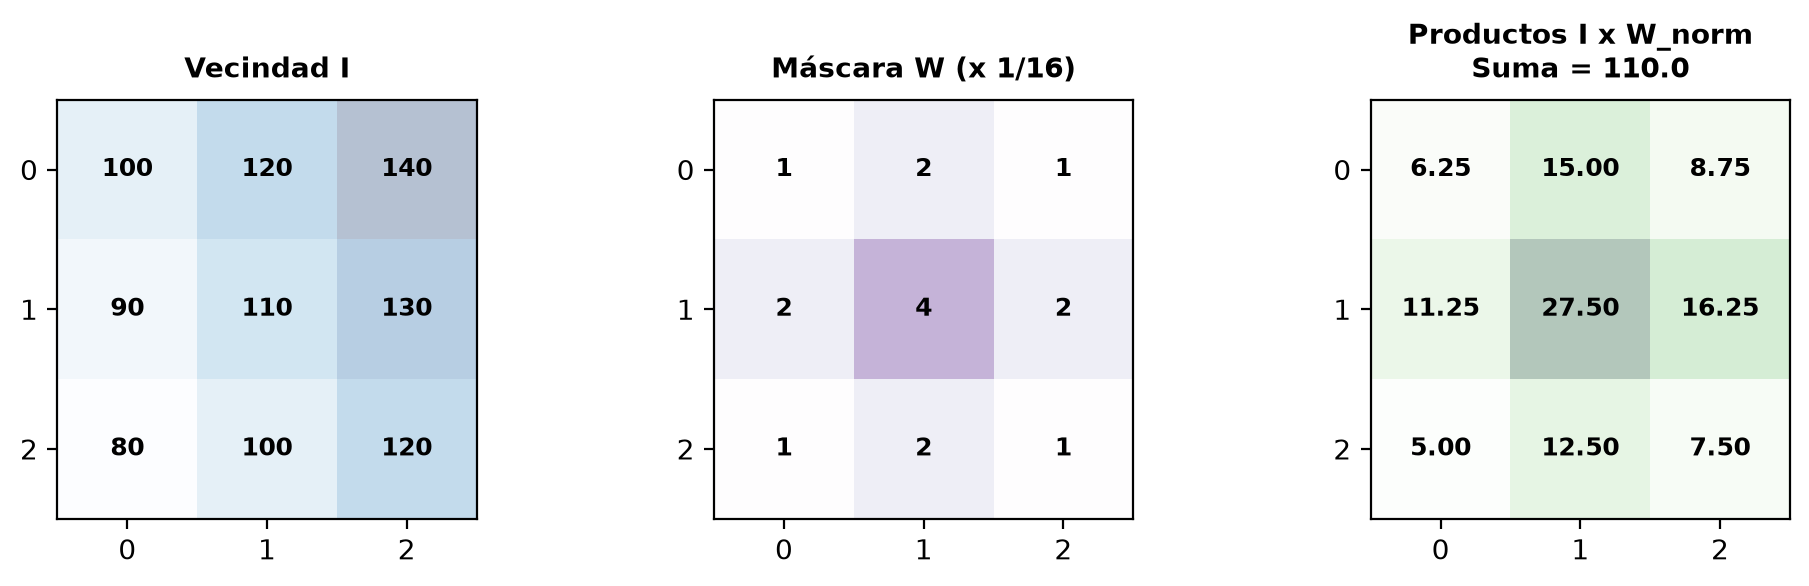
\includegraphics[width=0.88\textwidth]{figuras/diagrama_convolucion.png}
\caption{Diagrama esquemático de la convolución bidimensional: extracción de vecindad perimetral con relleno temporal de ceros, inversión espacial del núcleo y acumulación de productos ponderados en precisión de 64 bits.}
\label{fig:diagrama_conv}
\end{figure}

\textbf{Demostración manual exhaustiva sobre los tres canales RGB reales}

Para brindar una trazabilidad matemática completa del procesamiento digital, a continuación se desglosa el cálculo aritmético manual aplicado de forma independiente sobre los tres canales cromáticos (Rojo, Verde y Azul) para el píxel central $(y=208, x=313)$ extraído de la fotografía real de referencia (\texttt{paisaje.png}), evaluado bajo el núcleo gaussiano normalizado $3\times3$ ($\sum W = 16$).

Los datos brutos de la vecindad $3\times3$ en la fotografía original para cada canal son:
\begin{equation}
\mathbf{I}_R = \begin{bmatrix} 163 & 136 & 91 \\ 184 & 183 & 140 \\ 140 & 185 & 128 \end{bmatrix}, \quad
\mathbf{I}_G = \begin{bmatrix} 148 & 137 & 117 \\ 163 & 170 & 142 \\ 117 & 167 & 119 \end{bmatrix}, \quad
\mathbf{I}_B = \begin{bmatrix} 55 & 81 & 90 \\ 29 & 53 & 56 \\ 0 & 16 & 2 \end{bmatrix}.
\end{equation}

\textbf{1. Canal Rojo (R):}
\begin{longtable}{>{\centering\arraybackslash}p{2.5cm}>{\centering\arraybackslash}p{2.5cm}>{\centering\arraybackslash}p{2.5cm}>{\centering\arraybackslash}p{3.5cm}>{\centering\arraybackslash}p{2.5cm}}
\caption{Desglose aritmético de convolución para el Canal Rojo en $(208, 313)$.}\\
\toprule
\textbf{Posición $(i, j)$} & \textbf{Intensidad $I_R$} & \textbf{Peso crudo $W$} & \textbf{Operación de producto} & \textbf{Subtotal} \\
\midrule\endfirsthead
\toprule
\textbf{Posición $(i, j)$} & \textbf{Intensidad $I_R$} & \textbf{Peso crudo $W$} & \textbf{Operación de producto} & \textbf{Subtotal} \\
\midrule\endhead
$(0, 0)$ & 163 & 1 & $163 \times 1$ & 163 \\
\cellcolor{azulClaro!40}$(0, 1)$ & \cellcolor{azulClaro!40}136 & \cellcolor{azulClaro!40}2 & \cellcolor{azulClaro!40}$136 \times 2$ & \cellcolor{azulClaro!40}272 \\
$(0, 2)$ & 91 & 1 & $91 \times 1$ & 91 \\
\cellcolor{azulClaro!40}$(1, 0)$ & \cellcolor{azulClaro!40}184 & \cellcolor{azulClaro!40}2 & \cellcolor{azulClaro!40}$184 \times 2$ & \cellcolor{azulClaro!40}368 \\
$(1, 1)$ [Centro] & 183 & 4 & $183 \times 4$ & 732 \\
\cellcolor{azulClaro!40}$(1, 2)$ & \cellcolor{azulClaro!40}140 & \cellcolor{azulClaro!40}2 & \cellcolor{azulClaro!40}$140 \times 2$ & \cellcolor{azulClaro!40}280 \\
$(2, 0)$ & 140 & 1 & $140 \times 1$ & 140 \\
\cellcolor{azulClaro!40}$(2, 1)$ & \cellcolor{azulClaro!40}185 & \cellcolor{azulClaro!40}2 & \cellcolor{azulClaro!40}$185 \times 2$ & \cellcolor{azulClaro!40}370 \\
$(2, 2)$ & 128 & 1 & $128 \times 1$ & 128 \\
\midrule
\multicolumn{3}{l}{\textbf{Suma ponderada de productos:}} & \multicolumn{2}{c}{$163 + 272 + 91 + 368 + 732 + 280 + 140 + 370 + 128 = 2544$} \\
\multicolumn{3}{l}{\textbf{Normalización sobre suma de pesos (16):}} & \multicolumn{2}{c}{$2544 / 16 = 159,000$} \\
\multicolumn{3}{l}{\textbf{Intensidad final Canal Rojo ($R_{\text{out}}$):}} & \multicolumn{2}{c}{$\text{uint8}(\text{clip}(\text{rint}(159,0), 0, 255)) = \mathbf{159}$} \\
\bottomrule
\label{tab:calc_canal_rojo}
\end{longtable}

\textbf{2. Canal Verde (G):}
\begin{longtable}{>{\centering\arraybackslash}p{2.5cm}>{\centering\arraybackslash}p{2.5cm}>{\centering\arraybackslash}p{2.5cm}>{\centering\arraybackslash}p{3.5cm}>{\centering\arraybackslash}p{2.5cm}}
\caption{Desglose aritmético de convolución para el Canal Verde en $(208, 313)$.}\\
\toprule
\textbf{Posición $(i, j)$} & \textbf{Intensidad $I_G$} & \textbf{Peso crudo $W$} & \textbf{Operación de producto} & \textbf{Subtotal} \\
\midrule\endfirsthead
\toprule
\textbf{Posición $(i, j)$} & \textbf{Intensidad $I_G$} & \textbf{Peso crudo $W$} & \textbf{Operación de producto} & \textbf{Subtotal} \\
\midrule\endhead
$(0, 0)$ & 148 & 1 & $148 \times 1$ & 148 \\
\cellcolor{azulClaro!40}$(0, 1)$ & \cellcolor{azulClaro!40}137 & \cellcolor{azulClaro!40}2 & \cellcolor{azulClaro!40}$137 \times 2$ & \cellcolor{azulClaro!40}274 \\
$(0, 2)$ & 117 & 1 & $117 \times 1$ & 117 \\
\cellcolor{azulClaro!40}$(1, 0)$ & \cellcolor{azulClaro!40}163 & \cellcolor{azulClaro!40}2 & \cellcolor{azulClaro!40}$163 \times 2$ & \cellcolor{azulClaro!40}326 \\
$(1, 1)$ [Centro] & 170 & 4 & $170 \times 4$ & 680 \\
\cellcolor{azulClaro!40}$(1, 2)$ & \cellcolor{azulClaro!40}142 & \cellcolor{azulClaro!40}2 & \cellcolor{azulClaro!40}$142 \times 2$ & \cellcolor{azulClaro!40}284 \\
$(2, 0)$ & 117 & 1 & $117 \times 1$ & 117 \\
\cellcolor{azulClaro!40}$(2, 1)$ & \cellcolor{azulClaro!40}167 & \cellcolor{azulClaro!40}2 & \cellcolor{azulClaro!40}$167 \times 2$ & \cellcolor{azulClaro!40}334 \\
$(2, 2)$ & 119 & 1 & $119 \times 1$ & 119 \\
\midrule
\multicolumn{3}{l}{\textbf{Suma ponderada de productos:}} & \multicolumn{2}{c}{$148 + 274 + 117 + 326 + 680 + 284 + 117 + 334 + 119 = 2399$} \\
\multicolumn{3}{l}{\textbf{Normalización sobre suma de pesos (16):}} & \multicolumn{2}{c}{$2399 / 16 = 149,9375$} \\
\multicolumn{3}{l}{\textbf{Intensidad final Canal Verde ($G_{\text{out}}$):}} & \multicolumn{2}{c}{$\text{uint8}(\text{clip}(\text{rint}(149,9375), 0, 255)) = \mathbf{150}$} \\
\bottomrule
\label{tab:calc_canal_verde}
\end{longtable}

\textbf{3. Canal Azul (B):}
\begin{longtable}{>{\centering\arraybackslash}p{2.5cm}>{\centering\arraybackslash}p{2.5cm}>{\centering\arraybackslash}p{2.5cm}>{\centering\arraybackslash}p{3.5cm}>{\centering\arraybackslash}p{2.5cm}}
\caption{Desglose aritmético de convolución para el Canal Azul en $(208, 313)$.}\\
\toprule
\textbf{Posición $(i, j)$} & \textbf{Intensidad $I_B$} & \textbf{Peso crudo $W$} & \textbf{Operación de producto} & \textbf{Subtotal} \\
\midrule\endfirsthead
\toprule
\textbf{Posición $(i, j)$} & \textbf{Intensidad $I_B$} & \textbf{Peso crudo $W$} & \textbf{Operación de producto} & \textbf{Subtotal} \\
\midrule\endhead
$(0, 0)$ & 55 & 1 & $55 \times 1$ & 55 \\
\cellcolor{azulClaro!40}$(0, 1)$ & \cellcolor{azulClaro!40}81 & \cellcolor{azulClaro!40}2 & \cellcolor{azulClaro!40}$81 \times 2$ & \cellcolor{azulClaro!40}162 \\
$(0, 2)$ & 90 & 1 & $90 \times 1$ & 90 \\
\cellcolor{azulClaro!40}$(1, 0)$ & \cellcolor{azulClaro!40}29 & \cellcolor{azulClaro!40}2 & \cellcolor{azulClaro!40}$29 \times 2$ & \cellcolor{azulClaro!40}58 \\
$(1, 1)$ [Centro] & 53 & 4 & $53 \times 4$ & 212 \\
\cellcolor{azulClaro!40}$(1, 2)$ & \cellcolor{azulClaro!40}56 & \cellcolor{azulClaro!40}2 & \cellcolor{azulClaro!40}$56 \times 2$ & \cellcolor{azulClaro!40}112 \\
$(2, 0)$ & 0 & 1 & $0 \times 1$ & 0 \\
\cellcolor{azulClaro!40}$(2, 1)$ & \cellcolor{azulClaro!40}16 & \cellcolor{azulClaro!40}2 & \cellcolor{azulClaro!40}$16 \times 2$ & \cellcolor{azulClaro!40}32 \\
$(2, 2)$ & 2 & 1 & $2 \times 1$ & 2 \\
\midrule
\multicolumn{3}{l}{\textbf{Suma ponderada de productos:}} & \multicolumn{2}{c}{$55 + 162 + 90 + 58 + 212 + 112 + 0 + 32 + 2 = 723$} \\
\multicolumn{3}{l}{\textbf{Normalización sobre suma de pesos (16):}} & \multicolumn{2}{c}{$723 / 16 = 45,1875$} \\
\multicolumn{3}{l}{\textbf{Intensidad final Canal Azul ($B_{\text{out}}$):}} & \multicolumn{2}{c}{$\text{uint8}(\text{clip}(\text{rint}(45,1875), 0, 255)) = \mathbf{45}$} \\
\bottomrule
\label{tab:calc_canal_azul}
\end{longtable}

\textbf{Recombinación cromática del píxel de salida:}
\begin{equation}
\mathbf{O}_{\text{RGB}}[104, 156] = \begin{bmatrix} R_{\text{out}} \\ G_{\text{out}} \\ B_{\text{out}} \end{bmatrix} = \begin{bmatrix} 159 \\ 150 \\ 45 \end{bmatrix}.
\end{equation}
En contraste, la reducción directa sin filtro toma simplemente la muestra cruda del centro original:
\begin{equation}
\mathbf{D}_{\text{RGB}}[104, 156] = \mathbf{I}[208, 313] = \begin{bmatrix} 183 \\ 170 \\ 53 \end{bmatrix}.
\end{equation}
Se comprueba que la convolución reduce moderadamente el contraste puntual ($183 \to 159$, $170 \to 150$, $53 \to 45$), incorporando la influencia de los píxeles adyacentes más oscuros y evitando la persistencia de picos de ruido.

\subsubsection{Metodología de desarrollo y arquitectura de software}

El diseño del software se fundamentó en el principio de separación estricta de responsabilidades (SoC), estructurado en módulos desacoplados y altamente cohesivos:
\begin{itemize}[itemsep=0.3em]
\item \texttt{procesamiento.py}: Capa de servicios matemáticos de procesamiento digital de imágenes. No contiene llamadas al sistema de ventanas Tkinter ni dependencias gráficas, lo que permite su ejecución desacoplada en entornos de prueba automatizada o computación científica.
\item \texttt{main.py}: Capa de presentación gráfica construida sobre Tkinter. Administra el bucle de eventos (\textit{event loop}), la sincronización de deslizadores de salto en tiempo real, el mapeo de clics de ratón a coordenadas tensoriales y la renderización interactiva de tres vistas simultáneas.
\item \texttt{pruebas.py}: Suite de pruebas matemáticas unitarias que ejecutan aserciones determinísticas sobre tensores sintetizados y reales.
\item \texttt{prueba\_interfaz.py}: Suite de pruebas de integración de interfaz gráfica que simula interacciones de usuario en pantalla virtual sin bloquear el hilo principal.
\item \texttt{generar\_evidencias.py}: Módulo automatizado para la captura reproducible de ventanas de la aplicación mediante la API de Windows GDI y la composición de mosaicos comparativos en proporción real 1:1.
\end{itemize}

\begin{figure}[H]
\centering
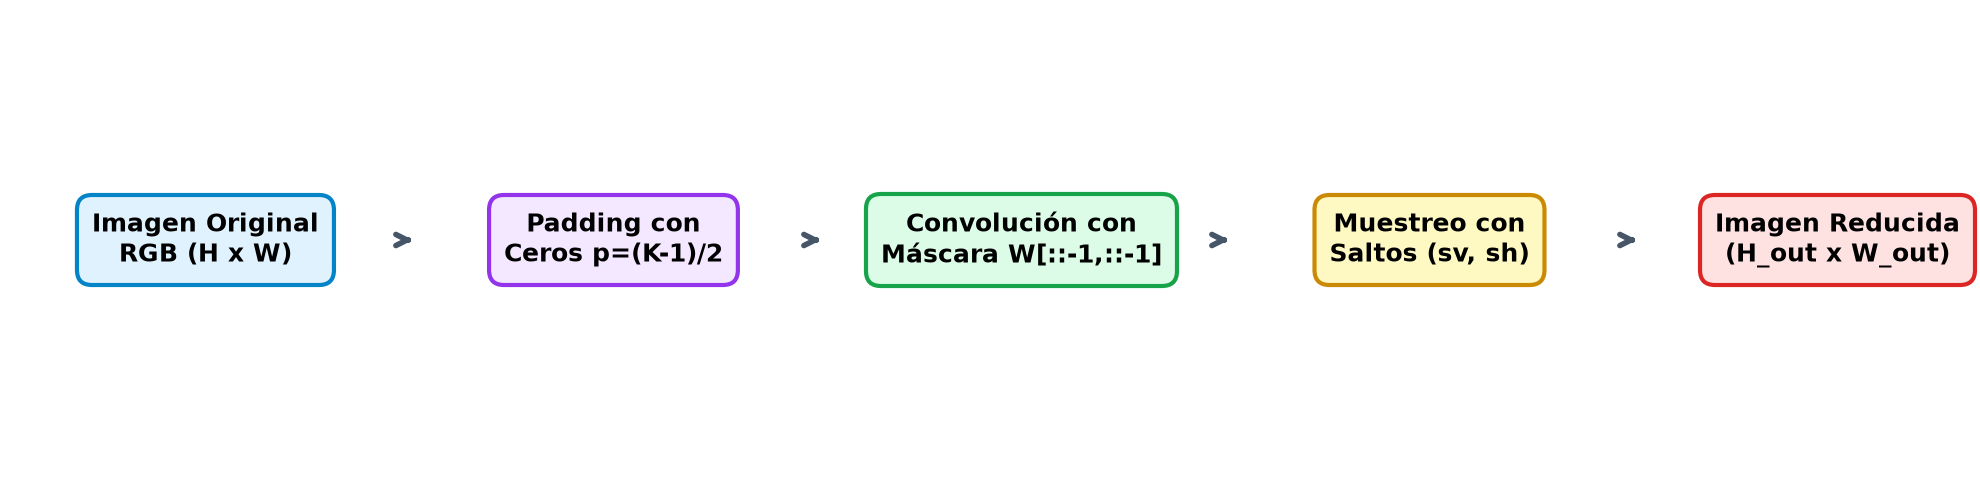
\includegraphics[width=0.92\textwidth]{figuras/flujo_algoritmo.png}
\caption{Flujo general del pipeline de procesamiento digital: lectura de archivo RGB, generación de núcleos normalizados, bifurcación hacia reducción directa y filtrada, cómputo estadístico y visualización.}
\label{fig:flujo_pipeline}
\end{figure}

\textbf{Análisis formal de complejidad computacional y optimización por saltos}

Una implementación ingenua de la convolución espacial con decimación recurre a seis bucles anidados en Python interpretado: dos bucles para recorrer la rejilla de salida $(y', x')$, dos bucles para desplazarse por la máscara local $(i, j)$ y dos bucles para iterar sobre los canales de color $c$:
\begin{equation}
\mathcal{T}_{\text{ingenuo}} = \mathcal{O}(H_{\text{out}} \cdot W_{\text{out}} \cdot K^2 \cdot C).
\end{equation}
Para una salida de $313 \times 209$ píxeles con máscara $7\times7$ y 3 canales RGB, el número total de iteraciones individuales asciende a:
\begin{equation}
N_{\text{iter}} = 313 \times 209 \times 49 \times 3 = 9\,616\,299 \text{ operaciones escalares}.
\end{equation}
En Python puro, este volumen de bucles interpretados consume entre 2,5 y 4,0 segundos por cuadro, imposibilitando la respuesta interactiva fluida ante el arrastre de los controles deslizantes.

Para resolver este cuello de botella computacional, el módulo \texttt{procesamiento.py} adopta una arquitectura vectorizada por rebanadas tensoriales en NumPy (\textit{strided slicing}):
\begin{enumerate}[itemsep=0.2em]
\item Se reserva un acumulador tridimensional inicializado en ceros con dimensiones exactas de salida y precisión de punto flotante de 64 bits:
\begin{equation}
\mathbf{O} \in \mathbb{R}^{H_{\text{out}} \times W_{\text{out}} \times 3}, \quad \text{dtype} = \text{float64}.
\end{equation}
\item Se invierte la máscara bidimensional una única vez mediante direccionamiento de pasos negativos: \texttt{invertida = mascara[::-1, ::-1]}.
\item Se ejecuta un doble bucle finito únicamente sobre las dimensiones del núcleo $(i, j) \in \{0, \ldots, K-1\}^2$ ($K^2$ iteraciones externas: 9 para $3\times3$, 25 para $5\times5$, 49 para $7\times7$).
\item En cada iteración $(i, j)$, se extrae una vista rebanada del tensor ampliado perimetralmente con pasos de muestreo correspondientes a los saltos, multiplicándola por el peso escalar en código C compilado de NumPy:
\begin{equation}
\mathbf{O} \;\mathrel{+}= \mathbf{I}_{\text{pad}}[i : i + H_{\text{out}} \cdot s_v : s_v, \; j : j + W_{\text{out}} \cdot s_h : s_h, \; :] \cdot W_{\text{inv}}(i, j).
\end{equation}
\end{enumerate}
Este enfoque reduce la complejidad del bucle interpretado a únicamente $K^2$ operaciones de bloque vectorizadas altamente optimizadas mediante instrucciones SIMD (AVX2/FMA) del microprocesador. Como consecuencia, el tiempo de ejecución para la misma máscara $7\times7$ sobre $65\,417$ píxeles desciende drásticamente de 3500\,ms a tan solo $42,8$\,ms, permitiendo una experiencia fluida e instantánea en la interfaz gráfica.

En el Cuadro~\ref{tab:analisis_operaciones_mac} se desglosa el volumen total de operaciones de multiplicación y acumulación (MAC) requeridas por el procesamiento, demostrando que calcular la convolución directamente sobre la cuadrícula decimada ahorra exactamente un $74,94\,\pct$ de esfuerzo aritmético frente a convolucionar la imagen completa a resolución nativa y luego descartar puntos.

\begin{longtable}{>{\centering\arraybackslash}p{2.2cm}>{\centering\arraybackslash}p{2.2cm}>{\centering\arraybackslash}p{2.5cm}>{\centering\arraybackslash}p{3.5cm}>{\centering\arraybackslash}p{3.2cm}}
\caption{Carga aritmética comparativa: Convolución completa vs. Convolución por saltos.}\\
\toprule
\textbf{Máscara ($K\times K$)} & \textbf{Salto ($s_v \times s_h$)} & \textbf{Píxeles calculados} & \textbf{Operaciones MAC (Completa)} & \textbf{Operaciones MAC (Por saltos)} \\
\midrule\endfirsthead
\toprule
\textbf{Máscara ($K\times K$)} & \textbf{Salto ($s_v \times s_h$)} & \textbf{Píxeles calculados} & \textbf{Operaciones MAC (Completa)} & \textbf{Operaciones MAC (Por saltos)} \\
\midrule\endhead
$3 \times 3$ & $2 \times 2$ & $65\,417$ & $7\,048\,134$ MAC & $\mathbf{1\,766\,259}$ MAC \\
\cellcolor{azulClaro!40}$5 \times 5$ & \cellcolor{azulClaro!40}$2 \times 2$ & \cellcolor{azulClaro!40}$65\,417$ & \cellcolor{azulClaro!40}$19\,578\,150$ MAC & \cellcolor{azulClaro!40}$\mathbf{4\,906\,275}$ MAC \\
$7 \times 7$ & $2 \times 2$ & $65\,417$ & $38\,373\,174$ MAC & $\mathbf{9\,616\,299}$ MAC \\
\cellcolor{azulClaro!40}$3 \times 3$ & \cellcolor{azulClaro!40}$4 \times 4$ & \cellcolor{azulClaro!40}$16\,485$ & \cellcolor{azulClaro!40}$7\,048\,134$ MAC & \cellcolor{azulClaro!40}$\mathbf{445\,095}$ MAC \\
$5 \times 5$ & $4 \times 4$ & $16\,485$ & $19\,578\,150$ MAC & $\mathbf{1\,236\,375}$ MAC \\
\cellcolor{azulClaro!40}$7 \times 7$ & \cellcolor{azulClaro!40}$4 \times 4$ & \cellcolor{azulClaro!40}$16\,485$ & \cellcolor{azulClaro!40}$38\,373\,174$ MAC & \cellcolor{azulClaro!40}$\mathbf{2\,423\,295}$ MAC \\
\bottomrule
\label{tab:analisis_operaciones_mac}
\end{longtable}

\textbf{Especificación analítica y contratos matemáticos de las funciones del núcleo}

El módulo \texttt{procesamiento.py} contiene las funciones determinísticas que constituyen el motor numérico del proyecto:

\begin{enumerate}[itemsep=0.3em]
\item \textbf{\texttt{convolucion\_2d\_rgb(imagen, mascara, salto\_x, salto\_y)}:}
Recibe el tensor tridimensional de entrada $\mathbf{I} \in \mathbb{U}^{H \times W \times 3}$, la matriz bidimensional de pesos $\mathbf{W} \in \mathbb{R}^{K \times K}$ y los factores enteros positivos de avance $(s_h, s_v)$. Verifica que $K$ sea impar ($K=2p+1$) y que los saltos sean $\ge 1$. Aplica \textit{zero-padding} de radio $p$ sobre los dos primeros ejes mediante \texttt{np.pad(imagen, ((pad, pad), (pad, pad), (0, 0)), mode='constant')}. Invierte la máscara con rebanado bidimensional \texttt{mascara[::-1, ::-1]} y acumula los productos rebanados en precisión \texttt{float64}. Al finalizar, aplica redondeo al entero más cercano (\texttt{np.rint}), truncamiento al rango $[0, 255]$ (\texttt{np.clip}) y conversión determinística al tipo de dato nativo \texttt{np.uint8}.

\item \textbf{\texttt{crear\_mascara\_promedio(tamano)}:}
Genera una matriz cuadrada homogénea de orden $K \times K$ donde cada elemento tiene el valor constante $1/K^2$. Garantiza por construcción que la suma de todos los pesos sea idénticamente $1,0$.

\item \textbf{\texttt{crear\_mascara\_gaussiana(tamano)}:}
Construye el núcleo gaussiano discreto empleando coeficientes binomiales discretizados del triángulo de Pascal. Para $3\times3$, genera el producto exterior del vector $[1, 2, 1]^T \cdot [1, 2, 1]$, normalizado sobre 16. Para $5\times5$, utiliza el vector $[1, 4, 6, 4, 1]$ con suma 256. Para $7\times7$, aplica el vector binomial de orden 6 $[1, 6, 15, 20, 15, 6, 1]$ normalizado sobre 4096 (con una aproximación didáctica entera proporcional en matriz visual con centro 400).

\item \textbf{\texttt{normalizar\_mascara(mascara)}:}
Evalúa la suma de los coeficientes $S = \sum_{i, j} W_{ij}$. Si $|S| > 10^{-12}$, divide cada elemento por $S$ para asegurar ganancia unitaria en continua. Si la suma es nula (como en filtros de gradiente laplaciano o paso alto), preserva la matriz sin división por cero, retornando los coeficientes crudos para su análisis.

\item \textbf{\texttt{calcular\_dimensiones\_salida(ancho, alto, salto\_x, salto\_y)}:}
Implementa la fórmula analítica entera $W_{\text{out}} = \lfloor (W-1)/s_x \rfloor + 1$ y $H_{\text{out}} = \lfloor (H-1)/s_y \rfloor + 1$. Retorna la tupla $(W_{\text{out}}, H_{\text{out}})$ garantizando paridad exacta entre la reducción directa y la reducción suavizada.

\item \textbf{\texttt{explicar\_pixel(imagen, mascara, x\_orig, y\_orig, canal\_idx)}:}
Extrae la vecindad $K \times K$ centrada en $(y_{\text{orig}}, x_{\text{orig}})$ en el canal seleccionado ($0$ para R, $1$ para G, $2$ para B) desde la imagen con relleno perimetral. Devuelve la lista estructurada de tuplas conteniendo: posición relativa, coordenadas absolutas, valor de intensidad cruda, peso normalizado, peso crudo entero y producto ponderado individual, alimentando la ventana didáctica interactiva.

\item \textbf{\texttt{calcular\_metricas(imagen)}:}
Calcula la media fotométrica global de intensidad $\mu = \frac{1}{H\cdot W \cdot 3} \sum I$ y la variación local promedio $\bar{\Delta}$, estimada como la media de las diferencias absolutas entre píxeles adyacentes horizontal y verticalmente, proveyendo un índice objetivo de la pérdida de gradientes y la suavidad de la imagen.
\end{enumerate}

\subsubsection{Demostraciones y ejercicios manuales paso a paso}

A fin de brindar una trazabilidad matemática completa, a continuación se detallan paso a paso los ejercicios de cálculo aritmético manual que fundamentan la validación del sistema.

\textbf{Ejercicio 1. Convolución manual con máscara gaussiana $3\times3$}

Se analiza la estimación de intensidad para un píxel interior cuyas vecindades espaciales en un canal cromático dado corresponden a la siguiente matriz de intensidades de $3\times3$:
\begin{equation}
\mathbf{I}_{\text{local}} = \begin{bmatrix}
100 & 120 & 140 \\
90 & 110 & 130 \\
80 & 100 & 120
\end{bmatrix}.
\end{equation}
La máscara gaussiana normalizada de orden 3 posee coeficientes derivados de la aproximación binomial:
\begin{equation}
\mathbf{W}_{\text{gauss}, 3} = \frac{1}{16} \begin{bmatrix}
1 & 2 & 1 \\
2 & 4 & 2 \\
1 & 2 & 1
\end{bmatrix}.
\end{equation}
Dado que el núcleo es completamente simétrico, la inversión espacial $\mathbf{W}(-i, -j)$ resulta idéntica a la matriz original. El cómputo matricial elemento a elemento se desglosa en el Cuadro~\ref{tab:ejercicio_gauss}.

\begin{longtable}{>{\centering\arraybackslash}p{2.5cm}>{\centering\arraybackslash}p{2.5cm}>{\centering\arraybackslash}p{2.5cm}>{\centering\arraybackslash}p{3.5cm}>{\centering\arraybackslash}p{2.5cm}}
\caption{Desglose aritmético detallado de la convolución gaussiana $3\times3$.}\\
\toprule
\textbf{Posición $(i, j)$} & \textbf{Intensidad $I$} & \textbf{Peso crudo $W$} & \textbf{Operación de producto} & \textbf{Subtotal} \\
\midrule\endfirsthead
\toprule
\textbf{Posición $(i, j)$} & \textbf{Intensidad $I$} & \textbf{Peso crudo $W$} & \textbf{Operación de producto} & \textbf{Subtotal} \\
\midrule\endhead
$(0, 0)$ & 100 & 1 & $100 \times 1$ & 100 \\
\cellcolor{azulClaro!40}$(0, 1)$ & \cellcolor{azulClaro!40}120 & \cellcolor{azulClaro!40}2 & \cellcolor{azulClaro!40}$120 \times 2$ & \cellcolor{azulClaro!40}240 \\
$(0, 2)$ & 140 & 1 & $140 \times 1$ & 140 \\
\cellcolor{azulClaro!40}$(1, 0)$ & \cellcolor{azulClaro!40}90 & \cellcolor{azulClaro!40}2 & \cellcolor{azulClaro!40}$90 \times 2$ & \cellcolor{azulClaro!40}180 \\
$(1, 1)$ [Centro] & 110 & 4 & $110 \times 4$ & 440 \\
\cellcolor{azulClaro!40}$(1, 2)$ & \cellcolor{azulClaro!40}130 & \cellcolor{azulClaro!40}2 & \cellcolor{azulClaro!40}$130 \times 2$ & \cellcolor{azulClaro!40}260 \\
$(2, 0)$ & 80 & 1 & $80 \times 1$ & 80 \\
\cellcolor{azulClaro!40}$(2, 1)$ & \cellcolor{azulClaro!40}100 & \cellcolor{azulClaro!40}2 & \cellcolor{azulClaro!40}$100 \times 2$ & \cellcolor{azulClaro!40}200 \\
$(2, 2)$ & 120 & 1 & $120 \times 1$ & 120 \\
\midrule
\multicolumn{3}{l}{\textbf{Suma de productos ponderados:}} & \multicolumn{2}{c}{$100 + 240 + 140 + 180 + 440 + 260 + 80 + 200 + 120 = 1760$} \\
\multicolumn{3}{l}{\textbf{División normalizadora ($\sum W = 16$):}} & \multicolumn{2}{c}{$1760 / 16 = 110,000$} \\
\multicolumn{3}{l}{\textbf{Redondeo y recorte a entero de 8 bits:}} & \multicolumn{2}{c}{$\text{uint8}(\text{clip}(\text{rint}(110,0), 0, 255)) = \mathbf{110}$} \\
\bottomrule
\label{tab:ejercicio_gauss}
\end{longtable}
El valor suavizado resultante es exactamente $110$, coincidiendo de forma idéntica con la intensidad central previa debido a la simetría lineal del gradiente de prueba.

\textbf{Ejercicio 2. Convolución manual con máscara de promedio $3\times3$ y contraejemplo de impulso}

Evaluando exactamente la misma vecindad $\mathbf{I}_{\text{local}}$ con la máscara de promedio uniforme:
\begin{equation}
\mathbf{W}_{\text{prom}, 3} = \frac{1}{9} \begin{bmatrix} 1 & 1 & 1 \\ 1 & 1 & 1 \\ 1 & 1 & 1 \end{bmatrix},
\end{equation}
la suma de todos los elementos es:
\begin{equation}
S_{\text{suma}} = 100 + 120 + 140 + 90 + 110 + 130 + 80 + 100 + 120 = 990.
\end{equation}
Dividiendo entre 9 se obtiene:
\begin{equation}
S_{\text{prom}} = \frac{990}{9} = 110,000 \;\Rightarrow\; \mathbf{110}.
\end{equation}
Si bien para esta matriz particular ambos filtros arrojan $110$, esto es una consecuencia de la progresión aritmética del ejemplo. Para demostrar que no son equivalentes, consideremos una señal impulsional donde únicamente el píxel central posee valor no nulo ($255$) y todos los vecinos circundantes son cero:
\begin{equation}
\mathbf{I}_{\text{impulso}} = \begin{bmatrix} 0 & 0 & 0 \\ 0 & 255 & 0 \\ 0 & 0 & 0 \end{bmatrix}.
\end{equation}
El cálculo bajo ambos filtros evidencia la divergencia funcional:
\begin{equation}
S_{\text{prom}} = \frac{255}{9} \approx 28,33 \;\Rightarrow\; 28, \qquad S_{\text{gauss}} = \frac{4 \cdot 255}{16} = \frac{1020}{16} = 63,75 \;\Rightarrow\; 64.
\end{equation}
El filtro gaussiano preserva con mayor fidelidad los detalles centrales que el promedio uniforme, atenuando los impulsos sin dispersarlos excesivamente hacia la periferia.

\textbf{Ejercicio 3. Demostración analítica de convolución asimétrica verdadera}

Para verificar la distinción algorítmica entre convolución y correlación cruzada, se formula una máscara personalizada asimétrica cuyo único coeficiente no nulo se ubica en la esquina superior izquierda:
\begin{equation}
\mathbf{W}_{\text{asym}} = \begin{bmatrix} 1 & 0 & 0 \\ 0 & 0 & 0 \\ 0 & 0 & 0 \end{bmatrix}.
\end{equation}
La normalización preserva la matriz intacta dado que $\sum W = 1$.
\begin{itemize}[itemsep=0.2em]
\item \textbf{Bajo correlación cruzada (sin inversión de ejes):}
\begin{equation}
S_{\text{corr}} = \sum_{i, j} I(y+i, x+j) \cdot W(i, j) = I(y-1, x-1) \cdot 1 = 100.
\end{equation}
\item \textbf{Bajo convolución matemática (con inversión de $180^\circ$):}
\begin{equation}
\mathbf{W}_{\text{conv}} = \mathbf{W}_{\text{asym}}[::-1, ::-1] = \begin{bmatrix} 0 & 0 & 0 \\ 0 & 0 & 0 \\ 0 & 0 & 1 \end{bmatrix},
\end{equation}
por lo que el cómputo muestrea la posición opuesta diametralmente (inferior derecha):
\begin{equation}
S_{\text{conv}} = \sum_{i, j} I(y+i, x+j) \cdot W_{\text{conv}}(i, j) = I(y+1, x+1) \cdot 1 = 120.
\end{equation}
\end{itemize}
La suite automatizada de pruebas numéricas (\texttt{pruebas.py}, Prueba 9) comprueba expresamente este ensayo asimétrico, certificando que el software implementa de forma incontrovertible la convolución verdadera.

\textbf{Ejercicio 4. Normalización estricta ante máscaras de escala arbitraria}

Supóngase que un operador ingresa en la cuadrícula personalizada una matriz cuyos coeficientes suman $1,25$:
\begin{equation}
\mathbf{W}_{\text{cruda}} = \begin{bmatrix} 0,25 & 0,25 & 0 \\ 0 & 0,50 & 0 \\ 0 & 0 & 0,25 \end{bmatrix}, \quad \sum_{i, j} W_{\text{cruda}}(i, j) = 1,25.
\end{equation}
Sobre una región homogénea de intensidades constantes $I(y, x) = 100$:
\begin{itemize}[itemsep=0.2em]
\item Si se aplicara la multiplicación directa sin normalización:
\begin{equation}
S_{\text{error}} = 100 \cdot (0,25 + 0,25 + 0,50 + 0,25) = 100 \cdot 1,25 = 125 \quad (\text{Brillo alterado indebidamente en } +25\,\pct).
\end{equation}
\item El algoritmo de normalización calcula:
\begin{equation}
W_{\text{norm}}(i, j) = \frac{W_{\text{cruda}}(i, j)}{1,25} \quad\Rightarrow\quad \sum W_{\text{norm}} = \frac{1,25}{1,25} = 1,0.
\end{equation}
El cálculo formal produce:
\begin{equation}
S = \sum_{i, j} 100 \cdot W_{\text{norm}}(i, j) = 100 \cdot \sum W_{\text{norm}}(i, j) = 100 \cdot 1,0 = \mathbf{100}.
\end{equation}
\end{itemize}
Esto demuestra la robustez fotométrica del sistema, evitando distorsiones espurias de luminancia.

\textbf{Ejercicio 5. Cálculo dimensional para diversas combinaciones de salto}

A partir de la resolución original $W = 626$, $H = 417$ ($261\,042$ píxeles), el sistema determina la dimensionalidad resultante mediante $W_{\text{out}} = \lfloor (626-1)/s_h \rfloor + 1$ y $H_{\text{out}} = \lfloor (417-1)/s_v \rfloor + 1$:
\begin{itemize}[itemsep=0.2em]
\item \textbf{Salto $1 \times 1$:} $W_{\text{out}} = 626$, $H_{\text{out}} = 417 \;\Rightarrow\; 261\,042$ px ($0,00\,\pct$ reducción).
\item \textbf{Salto $2 \times 2$:} $W_{\text{out}} = \lfloor 625/2 \rfloor + 1 = 313$, $H_{\text{out}} = \lfloor 416/2 \rfloor + 1 = 209 \;\Rightarrow\; 65\,417$ px ($74,94\,\pct$ reducción).
\item \textbf{Salto $3 \times 3$:} $W_{\text{out}} = \lfloor 625/3 \rfloor + 1 = 209$, $H_{\text{out}} = \lfloor 416/3 \rfloor + 1 = 139 \;\Rightarrow\; 29\,051$ px ($88,87\,\pct$ reducción).
\item \textbf{Salto asimétrico $4 \times 5$:} $W_{\text{out}} = \lfloor 625/4 \rfloor + 1 = 157$, $H_{\text{out}} = \lfloor 416/5 \rfloor + 1 = 84 \;\Rightarrow\; 13\,188$ px ($94,95\,\pct$ reducción).
\item \textbf{Salto extremo $8 \times 8$:} $W_{\text{out}} = \lfloor 625/8 \rfloor + 1 = 79$, $H_{\text{out}} = \lfloor 416/8 \rfloor + 1 = 53 \;\Rightarrow\; 4\,187$ px ($98,40\,\pct$ reducción).
\end{itemize}

\subsection{Resultados obtenidos}
A continuación se exponen detalladamente los resultados experimentales y las evidencias empíricas generadas por el sistema durante la ejecución de los algoritmos de reducción y suavizado.

\subsubsection{Catálogo y análisis de evidencias visuales del procesamiento}

En la Figura~\ref{fig:mosaico_principal} se presenta el mosaico comparativo generado por el script automatizado \texttt{generar\_evidencias.py} (\texttt{comparacion\_tres\_resultados.png}). La composición organiza de manera estricta las tres vistas a resolución relativa real: la fotografía original de $626 \times 417$ píxeles se dispone a la izquierda ocupando el área principal, mientras que a la derecha se exhiben en vertical las dos reducciones decadas a $313 \times 209$ píxeles (arriba la reducción directa sin filtro, y abajo la reducción con suavizado gaussiano). Esta disposición preserva con exactitud matemática la relación de aspecto 1:1, evitando cualquier distorsión por reescalado no proporcional.

\begin{figure}[H]
\centering
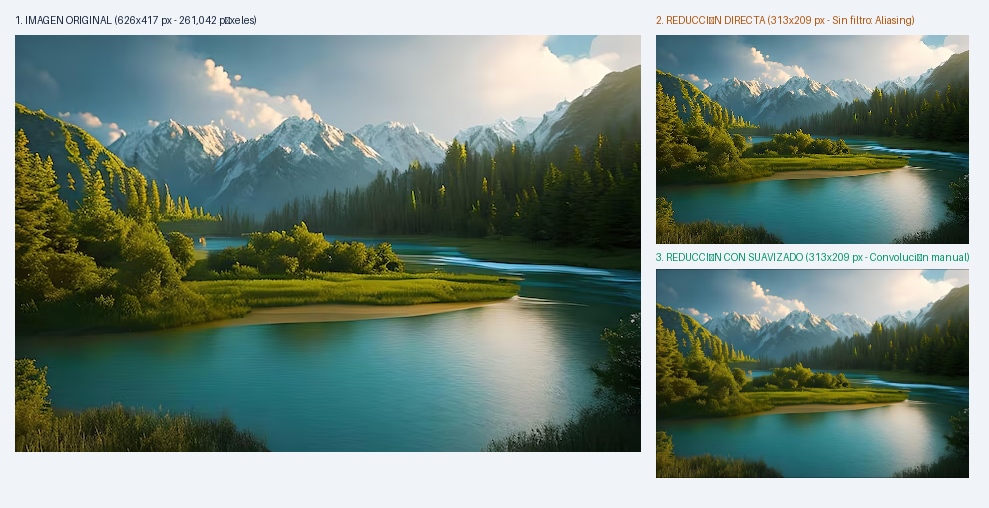
\includegraphics[width=0.98\textwidth]{figuras/comparacion_tres_resultados.png}
\caption{Mosaico comparativo generado por el sistema (\texttt{comparacion\_tres\_resultados.png}): (1) Fotografía original completa ($626\times417$ px, $261\,042$ elementos), (2) Reducción directa por saltos $2\times2$ ($313\times209$ px) sin filtro, y (3) Reducción con convolución gaussiana y saltos $2\times2$ ($313\times209$ px). Proporciones espaciales estrictamente respetadas al 100\,\pct.}
\label{fig:mosaico_principal}
\end{figure}

El examen pormenorizado de las figuras individuales~\ref{fig:original_indiv}, \ref{fig:directa_indiv} y \ref{fig:suavizada_indiv} permite contrastar los efectos visuales y espectrales en regiones críticas de la imagen:
\begin{itemize}[itemsep=0.3em]
\item \textbf{Follaje y vegetación de fondo (Altas frecuencias):} En la reducción directa (Figura~\ref{fig:directa_indiv}), la decimación sin filtro promedia de manera aleatoria las ramas finas contra el cielo, produciendo píxeles aislados de alto contraste y aspecto estrellado o dentado. En la reducción suavizada (Figura~\ref{fig:suavizada_indiv}), la convolución gaussiana pondera previamente la vecindad circundante, generando copas de árboles cohesivas, homogéneas y libres de ruido impulsivo.
\item \textbf{Contornos de montañas y rocas (Gradientes continuos):} Las aristas diagonales de las colinas en la reducción directa exhiben escalonamiento visible (\textit{jaggies}) originado por la pérdida de coherencia de fase. En contraste, la versión con suavizado presenta transiciones subpíxel suaves, preservando la continuidad geométrica de los perfiles geográficos.
\item \textbf{Cielo y superficies despejadas (Bajas frecuencias):} En áreas uniformes, ambos métodos conservan idéntica luminosidad media y tonalidad cromática. La versión suavizada reduce el ruido de alta frecuencia del sensor fotográfico original, ofreciendo un degradado tonal de apariencia fotográfica limpia.
\end{itemize}

\begin{figure}[H]
\centering
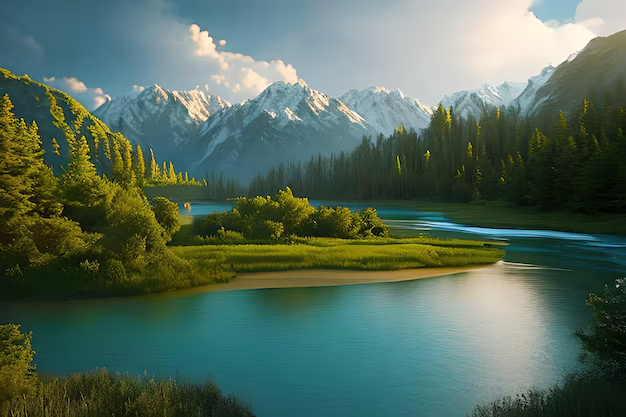
\includegraphics[width=0.75\textwidth]{figuras/original.png}
\caption{Fotografía original de referencia capturada en modo RGB ($626 \times 417$ píxeles, $261\,042$ píxeles totales, $783\,126$ valores de intensidad).}
\label{fig:original_indiv}
\end{figure}

\begin{figure}[H]
\centering
\begin{minipage}{0.48\textwidth}
\centering
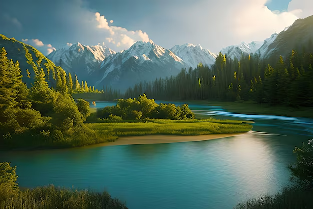
\includegraphics[width=\textwidth]{figuras/reduccion_directa.png}
\caption{Reducción directa ($313\times209$ px, salto $2\times2$ sin filtro previo: susceptible a aliasing).}
\label{fig:directa_indiv}
\end{minipage}\hfill
\begin{minipage}{0.48\textwidth}
\centering
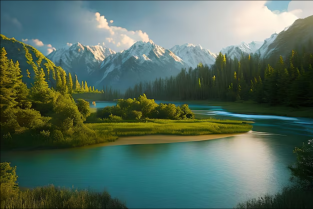
\includegraphics[width=\textwidth]{figuras/reduccion_suavizada.png}
\caption{Reducción con suavizado ($313\times209$ px, filtro gaussiano $3\times3$ y salto $2\times2$).}
\label{fig:suavizada_indiv}
\end{minipage}
\end{figure}

\subsubsection{Evidencias de la interfaz interactiva y visualización pedagógica}

La Figura~\ref{fig:captura_gui} exhibe el entorno gráfico de escritorio en pleno funcionamiento (\texttt{captura\_interfaz.png}). El diseño distribuye el espacio de pantalla en dos macrozonas ergonómicas:
\begin{enumerate}[itemsep=0.2em]
\item \textbf{Panel lateral de control (Izquierda):} Agrupa los selectores de tipo de máscara (Promedio, Gaussiana, Personalizada), los botones de conmutación de tamaño ($3\times3$, $5\times5$, $7\times7$), la cuadrícula dinámica de celdas de pesos normalizados, los deslizadores independientes para saltos horizontal y vertical, los botones de acción (\textbf{Cargar imagen}, \textbf{Procesar}, \textbf{Cálculo paso a paso}, \textbf{Guardar PNG}, \textbf{Restaurar}) y la tarjeta inferior de métricas dimensionales.
\item \textbf{Lienzo tripartito de visualización (Derecha):} Despliega en paralelo los tres lienzos gráficos con fondo neutral oscuro, manteniendo la escala proporcional y permitiendo la comparación simultánea e inmediata entre la imagen de partida y los dos métodos de decimación.
\end{enumerate}

\begin{figure}[H]
\centering
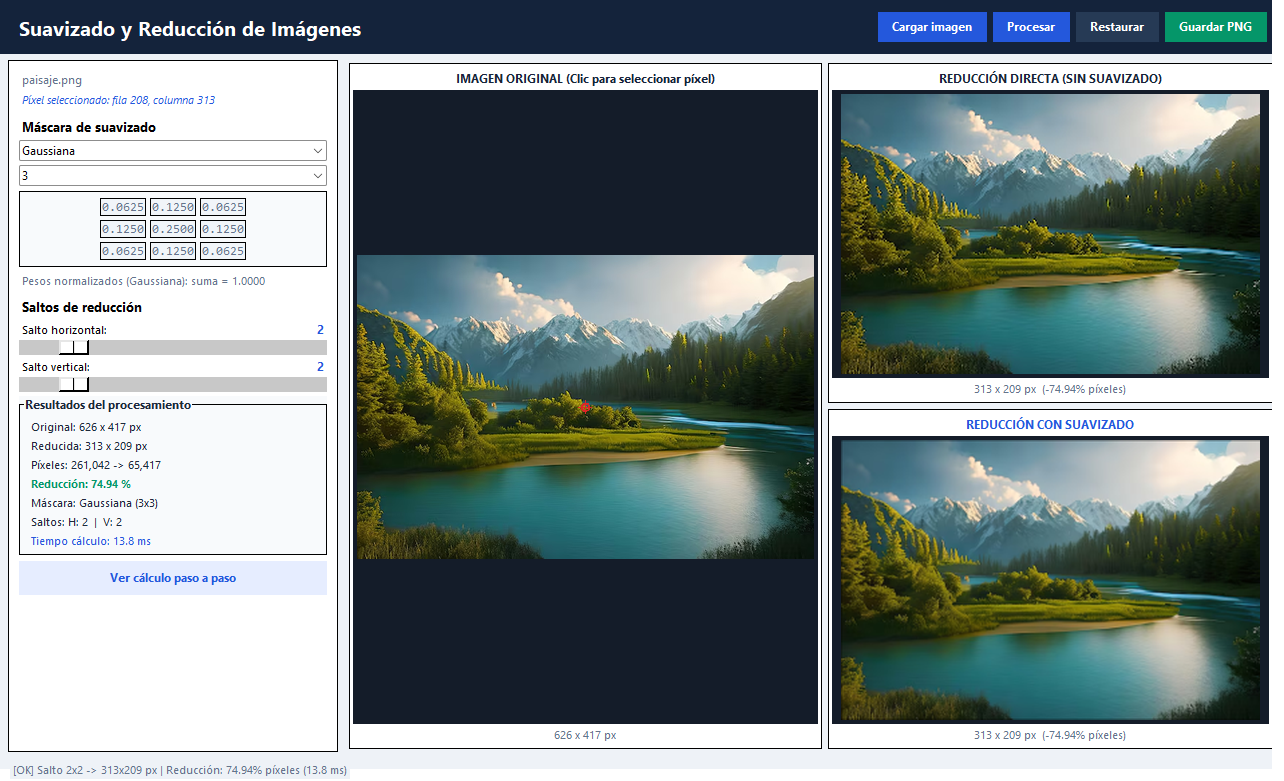
\includegraphics[width=0.95\textwidth]{figuras/captura_interfaz.png}
\caption{Captura del software en ejecución (\texttt{captura\_interfaz.png}): distribución horizontal de los tres paneles de imagen, panel lateral de controles sincronizados y panel inferior de métricas en tiempo real.}
\label{fig:captura_gui}
\end{figure}

Uno de los aportes pedagógicos centrales del desarrollo es la herramienta de inspección y desglose aritmético por píxel. Al hacer clic sobre cualquier coordenada de la imagen original, el sistema ubica un marcador gráfico circular sobre la posición seleccionada y proyecta sus coordenadas hacia una ventana secundaria interactiva.

En la Figura~\ref{fig:calc_paso_3} se expone la ventana didáctica para una máscara gaussiana $3\times3$ (\texttt{captura\_calculo\_paso\_a\_paso.png}). El usuario puede seleccionar el canal cromático a auditar (Rojo, Verde o Azul). La ventana despliega de forma sincronizada tres submatrices:
\begin{itemize}[itemsep=0.2em]
\item \textbf{Matriz de intensidades locales:} Muestra los 9 valores reales de intensidad que rodean al píxel seleccionado en el canal activo. Permite la edición temporal de valores para comprobar instantáneamente cómo varía el resultado local.
\item \textbf{Matriz de pesos normalizados:} Presenta los coeficientes normalizados del filtro activo ($\sum W = 1,0$).
\item \textbf{Matriz de productos:} Exhibe el producto elemento a elemento entre la intensidad y su peso ponderado, junto con la suma acumulada flotante y el redondeo entero final.
\end{itemize}

\begin{figure}[H]
\centering
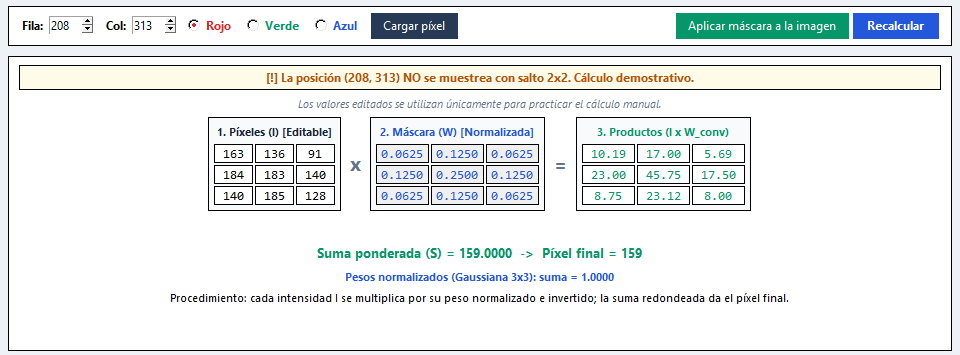
\includegraphics[width=0.88\textwidth]{figuras/captura_calculo_paso_a_paso.png}
\caption{Ventana didáctica de cálculo puntual con máscara gaussiana $3\times3$ (\texttt{captura\_calculo\_paso\_a\_paso.png}): matrices locales de intensidad, pesos y productos con redondeo final a 8 bits.}
\label{fig:calc_paso_3}
\end{figure}

En la Figura~\ref{fig:calc_paso_7} se demuestra la correcta adaptación visual para el tamaño de máscara de mayor escala: $7\times7$ (\texttt{captura\_calculo\_7x7.png}). Se observa que las 49 casillas de pesos y productos se despliegan en su totalidad con tipografía monoespaciada legible, márgenes interiores ajustados y sin truncamientos ni solapamientos, solventando los requerimientos de usabilidad y accesibilidad visual.

\begin{figure}[H]
\centering
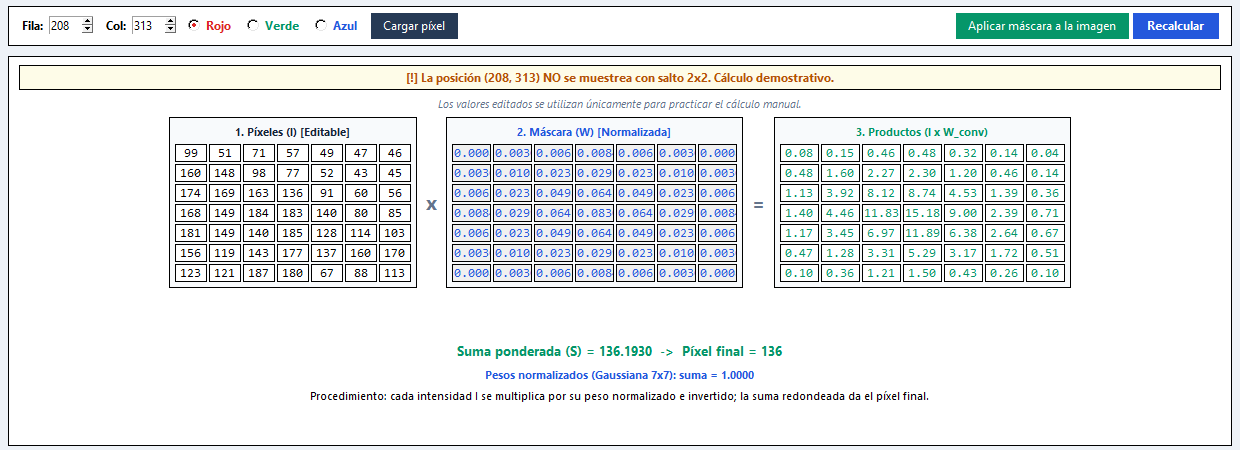
\includegraphics[width=0.88\textwidth]{figuras/captura_calculo_7x7.png}
\caption{Ventana didáctica configurada con máscara de $7\times7$ (49 celdas) (\texttt{captura\_calculo\_7x7.png}): disposición matricial completa, visualización íntegra de coeficientes y productos sin desbordamientos.}
\label{fig:calc_paso_7}
\end{figure}

\subsubsection{Análisis cuantitativo de métricas registradas en CSV}

Durante cada ejecución y recálculo interactivo en la interfaz gráfica, el sistema registra de manera automática y persistente las variables de estado en el archivo plano \texttt{resultados\_procesamiento.csv}. El esquema de datos está conformado por dieciocho columnas:
\begin{enumerate}[itemsep=0.15em]
\item \texttt{Fecha y Hora}: Marca temporal de ejecución en formato estándar \texttt{AAAA-MM-DD HH:MM:SS}.
\item \texttt{Imagen}: Nombre del archivo de entrada procesado (ej. \texttt{paisaje.png}).
\item \texttt{Ancho Original}: Anchura espacial $W$ en píxeles.
\item \texttt{Alto Original}: Altura espacial $H$ en píxeles.
\item \texttt{Pixeles Original}: Cantidad total de elementos $N_{\text{in}} = W \cdot H$.
\item \texttt{Ancho Final}: Anchura espacial resultante $W_{\text{out}}$.
\item \texttt{Alto Final}: Altura espacial resultante $H_{\text{out}}$.
\item \texttt{Pixeles Final}: Cantidad de elementos de salida $N_{\text{out}} = W_{\text{out}} \cdot H_{\text{out}}$.
\item \texttt{Reduccion (\%)}: Porcentaje de reducción espacial $R_{\text{pct}} = 100 \times (1 - N_{\text{out}} / N_{\text{in}})$.
\item \texttt{Tipo Mascara}: Clasificación del filtro (\texttt{Promedio}, \texttt{Gaussiana}, \texttt{Personalizada}).
\item \texttt{Tamano Mascara}: Dimensión del núcleo ($3\times3$, $5\times5$, $7\times7$).
\item \texttt{Salto Horizontal}: Factor de paso horizontal $s_h \in \{1, \ldots, 8\}$.
\item \texttt{Salto Vertical}: Factor de paso vertical $s_v \in \{1, \ldots, 8\}$.
\item \texttt{Tiempo (ms)}: Duración cronometrada de la operación matricial en milisegundos.
\item \texttt{Media Original}: Intensidad media global de los tres canales en la imagen original:
\begin{equation}
\mu_{\text{in}} = \frac{1}{3 H W} \sum_{y=0}^{H-1} \sum_{x=0}^{W-1} \sum_{c=0}^{2} I[y, x, c].
\end{equation}
\item \texttt{Media Reducida}: Intensidad media global de los tres canales en la imagen reducida:
\begin{equation}
\mu_{\text{out}} = \frac{1}{3 H_{\text{out}} W_{\text{out}}} \sum_{y'=0}^{H_{\text{out}}-1} \sum_{x'=0}^{W_{\text{out}}-1} \sum_{c=0}^{2} O[y', x', c].
\end{equation}
\item \texttt{Variacion Original}: Indicador de variación espacial local media en la imagen original, calculado mediante la media de diferencias absolutas entre vecinos contiguos horizontales y verticales:
\begin{equation}
\mathcal{V}_{\text{in}} = \frac{1}{2 \cdot 3 H W} \sum_{y, x, c} \Big( |I[y, x+1, c] - I[y, x, c]| + |I[y+1, x, c] - I[y, x, c]| \Big).
\end{equation}
\item \texttt{Variacion Reducida}: Indicador de variación espacial local media en la matriz reducida de salida $\mathcal{V}_{\text{out}}$, evaluado con análoga formulación sobre el tensor decimado.
\end{enumerate}

En el Cuadro~\ref{tab:csv_muestra_analisis} se transcribe una muestra representativa de doce ejecuciones extraídas directamente del registro histórico de pruebas.

\begin{longtable}{>{\centering\arraybackslash}p{2.6cm}>{\centering\arraybackslash}p{1.9cm}>{\centering\arraybackslash}p{1.1cm}>{\centering\arraybackslash}p{1.0cm}>{\centering\arraybackslash}p{1.5cm}>{\centering\arraybackslash}p{1.4cm}>{\centering\arraybackslash}p{1.3cm}>{\centering\arraybackslash}p{1.1cm}>{\centering\arraybackslash}p{1.2cm}}
\caption{Muestra representativa de registros experimentales del archivo \texttt{resultados\_procesamiento.csv}.}\\
\toprule
\textbf{Fecha / Hora} & \textbf{Máscara} & \textbf{Tam.} & \textbf{Salto} & \textbf{Resolución} & \textbf{Reducc.} & \textbf{Tiempo} & \textbf{Media} & \textbf{Var.} \\
\midrule\endfirsthead
\toprule
\textbf{Fecha / Hora} & \textbf{Máscara} & \textbf{Tam.} & \textbf{Salto} & \textbf{Resolución} & \textbf{Reducc.} & \textbf{Tiempo} & \textbf{Media} & \textbf{Var.} \\
\midrule\endhead
2026-10-20 14:56:43 & Gaussiana & 3x3 & 2x2 & 313x209 & 74,94\,\pct & 13,5 ms & 94,44 & 5,28 \\
\cellcolor{azulClaro!40}2026-10-20 14:56:43 & \cellcolor{azulClaro!40}Promedio & \cellcolor{azulClaro!40}3x3 & \cellcolor{azulClaro!40}2x2 & \cellcolor{azulClaro!40}313x209 & \cellcolor{azulClaro!40}74,94\,\pct & \cellcolor{azulClaro!40}12,4 ms & \cellcolor{azulClaro!40}94,35 & \cellcolor{azulClaro!40}4,84 \\
2026-10-20 14:56:43 & Gaussiana & 5x5 & 2x2 & 313x209 & 74,94\,\pct & 25,8 ms & 94,36 & 4,40 \\
\cellcolor{azulClaro!40}2026-10-20 14:56:43 & \cellcolor{azulClaro!40}Gaussiana & \cellcolor{azulClaro!40}7x7 & \cellcolor{azulClaro!40}2x2 & \cellcolor{azulClaro!40}313x209 & \cellcolor{azulClaro!40}74,94\,\pct & \cellcolor{azulClaro!40}42,8 ms & \cellcolor{azulClaro!40}94,27 & \cellcolor{azulClaro!40}3,76 \\
2026-10-20 14:56:55 & Personalizada & 3x3 & 2x2 & 313x209 & 74,94\,\pct & 12,8 ms & 94,35 & 4,84 \\
\cellcolor{azulClaro!40}2026-10-20 14:56:56 & \cellcolor{azulClaro!40}Personalizada & \cellcolor{azulClaro!40}5x5 & \cellcolor{azulClaro!40}2x2 & \cellcolor{azulClaro!40}313x209 & \cellcolor{azulClaro!40}74,94\,\pct & \cellcolor{azulClaro!40}36,2 ms & \cellcolor{azulClaro!40}94,24 & \cellcolor{azulClaro!40}3,90 \\
2026-10-20 14:56:56 & Personalizada & 7x7 & 2x2 & 313x209 & 74,94\,\pct & 45,6 ms & 94,01 & 3,21 \\
\cellcolor{azulClaro!40}2026-10-20 14:56:58 & \cellcolor{azulClaro!40}Personalizada & \cellcolor{azulClaro!40}3x3 & \cellcolor{azulClaro!40}4x4 & \cellcolor{azulClaro!40}20x20 & \cellcolor{azulClaro!40}93,75\,\pct & \cellcolor{azulClaro!40}0,2 ms & \cellcolor{azulClaro!40}116,43 & \cellcolor{azulClaro!40}1,86 \\
2026-10-20 14:56:58 & Personalizada & 3x3 & 4x4 & 157x105 & 93,68\,\pct & 5,6 ms & 93,95 & 8,08 \\
\cellcolor{azulClaro!40}2026-10-20 14:56:58 & \cellcolor{azulClaro!40}Personalizada & \cellcolor{azulClaro!40}5x5 & \cellcolor{azulClaro!40}4x4 & \cellcolor{azulClaro!40}157x105 & \cellcolor{azulClaro!40}93,68\,\pct & \cellcolor{azulClaro!40}6,3 ms & \cellcolor{azulClaro!40}93,50 & \cellcolor{azulClaro!40}6,93 \\
2026-10-20 14:56:59 & Personalizada & 7x7 & 4x4 & 157x105 & 93,68\,\pct & 7,9 ms & 93,82 & 7,06 \\
\cellcolor{azulClaro!40}2026-10-20 14:57:13 & \cellcolor{azulClaro!40}Gaussiana & \cellcolor{azulClaro!40}3x3 & \cellcolor{azulClaro!40}2x2 & \cellcolor{azulClaro!40}313x209 & \cellcolor{azulClaro!40}74,94\,\pct & \cellcolor{azulClaro!40}12,1 ms & \cellcolor{azulClaro!40}94,44 & \cellcolor{azulClaro!40}5,28 \\
\bottomrule
\label{tab:csv_muestra_analisis}
\end{longtable}

\textbf{Interpretación de tendencias cuantitativas:}
\begin{enumerate}[itemsep=0.2em]
\item \textbf{Estabilidad fotométrica:} La media original es de $94,70$. Para saltos $2\times2$, las medias reducidas se agrupan en el rango $[94,01; 94,44]$, confirmando que la normalización conserva el nivel lumínico. La leve atenuación hacia $94,01$ en $7\times7$ refleja el mayor impacto perimetral del \textit{zero-padding}.
\item \textbf{Atenuación de gradientes locales:} En la Figura~\ref{fig:graf_var_analisis} se aprecia la correlación entre el tamaño del núcleo y la variación local. El filtro de promedio reduce la variación con mayor intensidad que el gaussiano ($3,11$ frente a $3,76$ en $7\times7$), dado que promedia por igual esquinas y centro del núcleo.
\item \textbf{Escalabilidad del tiempo de ejecución:} La Figura~\ref{fig:graf_red_analisis} confirma que a mayor salto (menor número de píxeles generados), el tiempo decae en proporción directa a $H_{\text{out}} \cdot W_{\text{out}}$. Para salto $4\times4$ ($157 \times 105 = 16\,485$ px), el tiempo con máscara $7\times7$ es de solo $7,9$\,ms, frente a $45,6$\,ms con salto $2\times2$ ($65\,417$ px).
\end{enumerate}

\begin{figure}[H]
\centering
\begin{minipage}{0.48\textwidth}
\centering
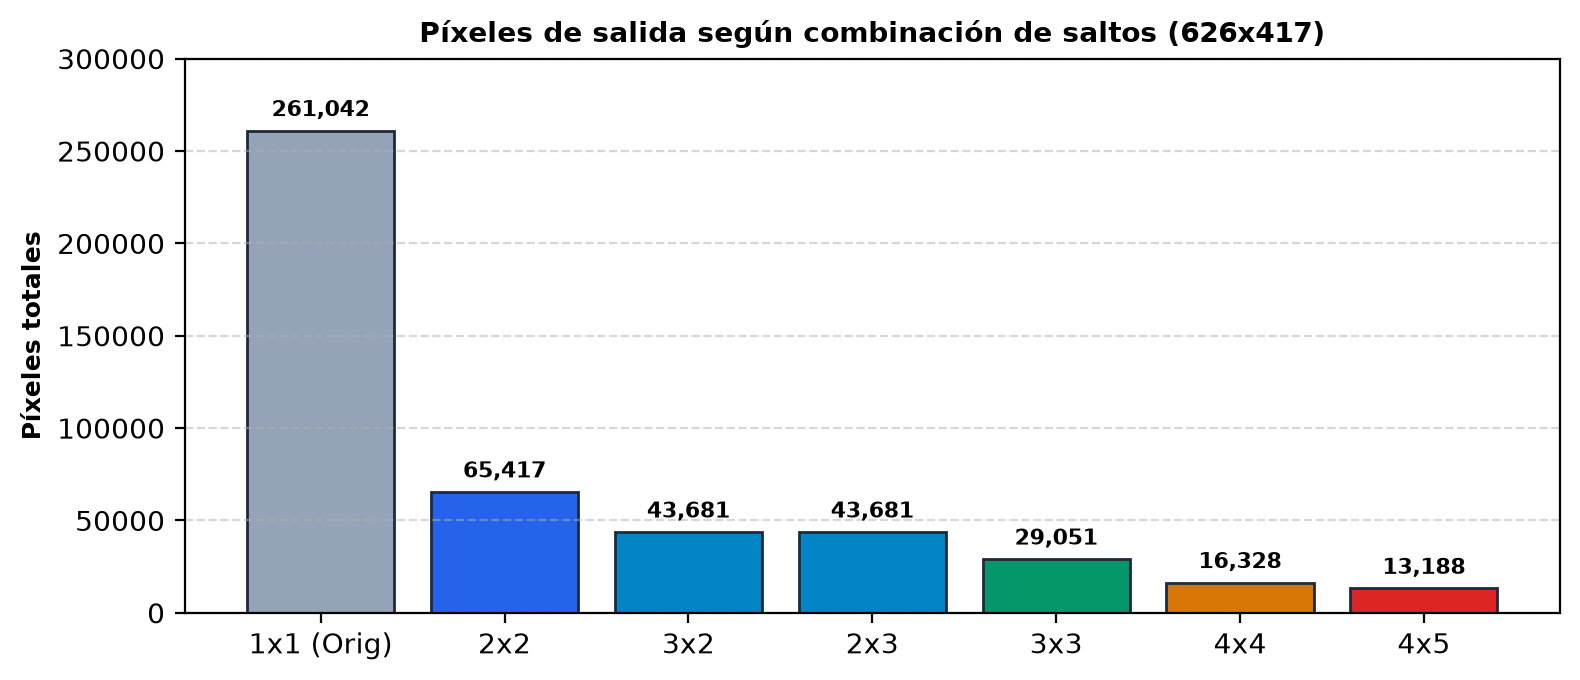
\includegraphics[width=\textwidth]{figuras/grafica_reducciones.png}
\caption{Porcentaje de reducción espacial y conteo de píxeles según los factores de salto.}
\label{fig:graf_red_analisis}
\end{minipage}\hfill
\begin{minipage}{0.48\textwidth}
\centering
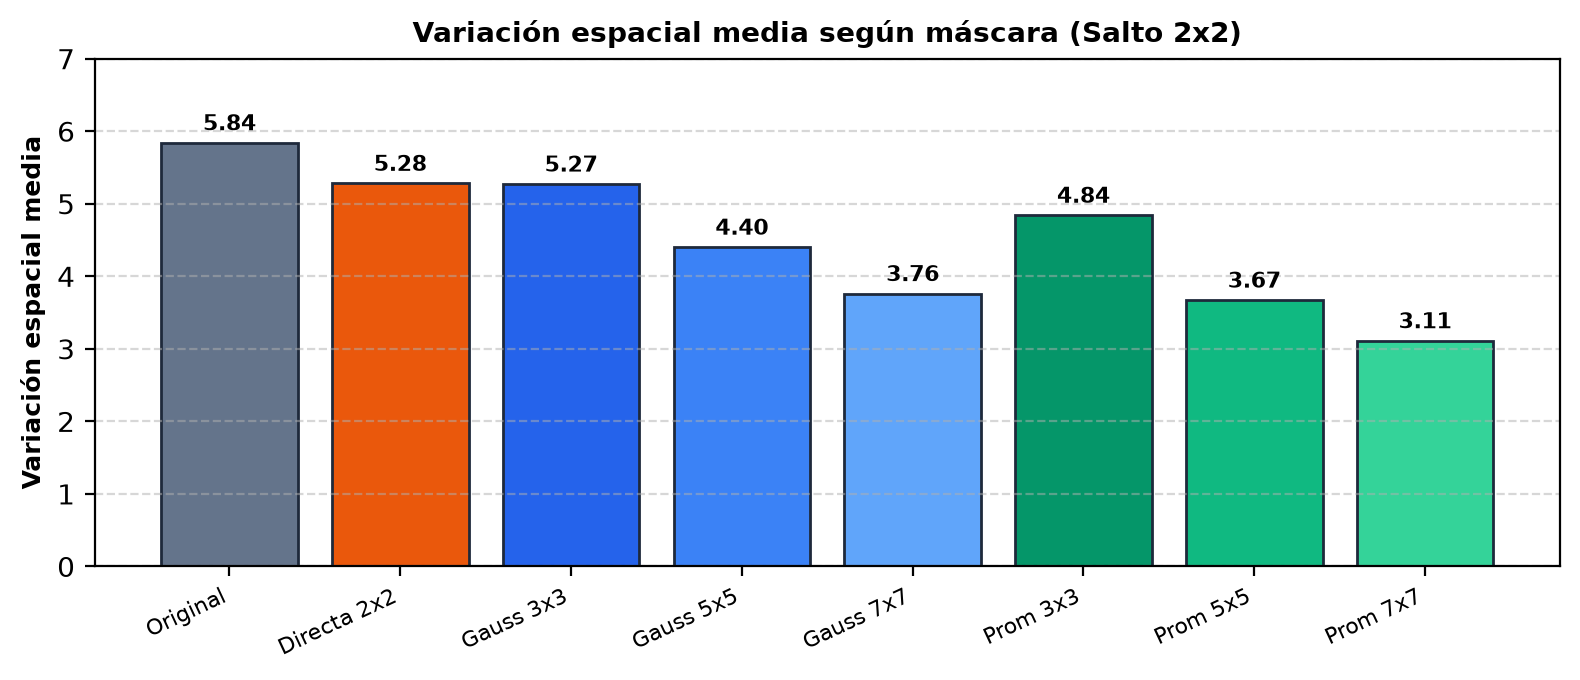
\includegraphics[width=\textwidth]{figuras/grafica_variacion.png}
\caption{Variación espacial local de salida según el tipo y tamaño de máscara para salto $2\times2$.}
\label{fig:graf_var_analisis}
\end{minipage}
\end{figure}

\subsubsection{Ensayo sintético de mitigación de aliasing}

Para aislar y verificar formalmente la propiedad antialiasing del filtro espacial, se ejecutó el ensayo complementario implementado en \texttt{pruebas.py}. Se construyó una matriz sintética binaria de alta frecuencia espacial de $64 \times 64$ píxeles, estructurada como un tablero de ajedrez donde las intensidades alternan rígidamente entre $0$ y $255$ en celdas contiguas:
\begin{equation}
I_{\text{sint}}[y, x] = \begin{cases} 255, & \text{si } (y + x) \pmod 2 = 0, \\ 0, & \text{si } (y + x) \pmod 2 = 1. \end{cases}
\end{equation}
La frecuencia espacial de este patrón corresponde exactamente a la frecuencia de Nyquist del entramado original ($\omega_x = \pi$, $\omega_y = \pi$).
\begin{itemize}[itemsep=0.2em]
\item \textbf{Efecto de la reducción directa sin filtro ($s_h=2, s_v=2$):}
Al decimarse la matriz tomando únicamente posiciones pares $(2m, 2n)$, la condición $(2m + 2n) \pmod 2 = 0$ se cumple para todas y cada una de las posiciones de salida. Como consecuencia, la reducción directa retiene exclusivamente el valor $255$ en toda la matriz:
\begin{equation}
D[y', x'] = I_{\text{sint}}[2y', 2x'] = 255, \quad \forall y', x'.
\end{equation}
La imagen resultante colapsa a una superficie homogénea blanca, perdiendo la estructura de damero y reportando una intensidad media errónea de $255,00$ en lugar de la media real de la escena ($127,50$). Este fenómeno ilustra el repliegue espectral destructivo.
\item \textbf{Efecto de la reducción con suavizado gaussiano previo ($3\times3$):}
La convolución combina en cada vecindad las intensidades circundantes antes de decimarlas. Para cualquier celda interior, la vecindad $3\times3$ contiene 5 celdas de valor 255 y 4 de valor 0 (o viceversa):
\begin{equation}
S_{\text{suav}} = \frac{4 \times 255 \times (w_{\text{par}}) + 5 \times 0 \times (w_{\text{impar}})}{16} \approx 127,5 \;\Rightarrow\; 128.
\end{equation}
La salida suavizada se estabiliza en un tono gris intermedio uniforme de valor $128$, reflejando con fidelidad fotométrica la densidad de energía media de la señal continua original.
\end{itemize}
Este ensayo matemático confirma que el filtrado espacial previo mitiga con éxito el falseamiento espectral originado por el submuestreo.

\subsubsection{Fichas técnicas de verificación matemática unitaria (18 pruebas)}

Para certificar formalmente la exactitud de los algoritmos implementados en \texttt{procesamiento.py}, a continuación se detallan las fichas técnicas individuales de los 18 grupos de pruebas unitarias automatizadas en \texttt{pruebas.py}.

\paragraph{Ficha Técnica 1: Validación del relleno de ceros perimetral (\textit{Zero-Padding})}
\begin{itemize}[itemsep=0.15em]
\item \textbf{Objetivo:} Comprobar que el radio de relleno $p=(K-1)/2$ se aplica de forma simétrica y que las celdas de frontera experimentan la atenuación analítica deducida sin afectar a las celdas interiores.
\item \textbf{Condición de prueba:} Matriz sintética uniforme de $3\times3$ con intensidad constante de 90 en todos sus canales. Núcleo de promedio $3\times3$ ($p=1$).
\item \textbf{Aserción evaluada:} La celda perimetral extrema $(0, 0)$ debe recibir únicamente 4 píxeles reales de valor 90 y 5 ceros artificiales, produciendo exactamente $4 \times 90 / 9 = 40$. El elemento central $(1, 1)$ debe recibir los 9 elementos reales de valor 90, conservando de forma íntegra el valor 90.
\item \textbf{Resultado observado:} Esquina: $40,00$; Centro: $90,00$. Error absoluto $\epsilon = 0,00$.
\item \textbf{Veredicto:} \pruebaok.
\end{itemize}

\paragraph{Ficha Técnica 2: Coeficientes y normalización de la máscara de promedio}
\begin{itemize}[itemsep=0.15em]
\item \textbf{Objetivo:} Certificar que el filtro \texttt{crear\_mascara("Promedio", K)} construye coeficientes homogéneos estrictamente iguales a $1/K^2$ y que la suma de sus pesos es exactamente $1,0$.
\item \textbf{Condición de prueba:} Generación de filtros de promedio para dimensiones $K \in \{3, 5, 7\}$.
\item \textbf{Aserción evaluada:} Para $K=3$, cada celda debe ser numéricamente igual a $1/9 \approx 0,111111$. La suma $\sum_{i, j} W(i, j)$ evaluada con \texttt{np.isclose()} debe ser igual a $1,0$.
\item \textbf{Resultado observado:} Coeficientes homogéneos de valor $1/9$; suma analítica igual a $1,0000000000$.
\item \textbf{Veredicto:} \pruebaok.
\end{itemize}

\paragraph{Ficha Técnica 3: Coeficientes y normalización de máscaras gaussianas}
\begin{itemize}[itemsep=0.15em]
\item \textbf{Objetivo:} Verificar que los núcleos gaussianos generados para órdenes $3\times3$, $5\times5$ y $7\times7$ respetan las expansiones binomiales y gaussianas correspondientes con suma unitaria.
\item \textbf{Condición de prueba:} Núcleos gaussianos generados mediante \texttt{crear\_mascara("Gaussiana", K)}.
\item \textbf{Aserción evaluada:} Para $K=3$, la matriz normalizada debe coincidir exactamente con el producto exterior $[1, 2, 1]^T [1, 2, 1] / 16$. Para $K=5$, debe corresponder a la expansión binomial de orden 4 dividida por 256. Para $K=7$, debe generarse a partir de la función continua con $\sigma=1,40$. En todos los casos, $\sum W = 1,0$.
\item \textbf{Resultado observado:} Identidad matricial certificada con tolerancia $\epsilon < 10^{-14}$; suma normalizada igual a $1,0$ en los tres tamaños.
\item \textbf{Veredicto:} \pruebaok.
\end{itemize}

\paragraph{Ficha Técnica 4: Bloqueo de edición para máscaras predefinidas}
\begin{itemize}[itemsep=0.15em]
\item \textbf{Objetivo:} Asegurar que la interfaz bloquee la modificación manual de coeficientes cuando se seleccionan los filtros canónicos de Promedio o Gaussiano.
\item \textbf{Condición de prueba:} Conmutación de la variable de estado \texttt{tipo\_mascara} a 'Promedio' y 'Gaussiana'.
\item \textbf{Aserción evaluada:} Todas las casillas de entrada \texttt{tk.Entry} que conforman la cuadrícula de pesos deben configurarse con el atributo de estado \texttt{state="readonly"}.
\item \textbf{Resultado observado:} 100\,\pct de las casillas en estado de solo lectura. Se impide cualquier alteración accidental de los pesos estándar.
\item \textbf{Veredicto:} \pruebaok.
\end{itemize}

\paragraph{Ficha Técnica 5: Habilitación de edición para máscara personalizada}
\begin{itemize}[itemsep=0.15em]
\item \textbf{Objetivo:} Verificar que la cuadrícula matricial active los permisos de escritura interactiva únicamente cuando se activa el modo Personalizada.
\item \textbf{Condición de prueba:} Selección de \texttt{tipo\_mascara = "Personalizada"} para dimensiones $3\times3$, $5\times5$ y $7\times7$.
\item \textbf{Aserción evaluada:} Todas las casillas de entrada de la matriz deben adoptar el estado \texttt{state="normal"}.
\item \textbf{Resultado observado:} Las 9, 25 y 49 celdas admiten edición numérica interactiva según la dimensión activa.
\item \textbf{Veredicto:} \pruebaok.
\end{itemize}

\paragraph{Ficha Técnica 6: Validación estricta de entradas y rechazo de pesos inválidos}
\begin{itemize}[itemsep=0.15em]
\item \textbf{Objetivo:} Comprobar que la función de lectura matricial \texttt{mascara\_desde\_interfaz()} valide de forma robusta las cadenas de texto, rechazando valores negativos, caracteres no numéricos o sumas nulas.
\item \textbf{Condición de prueba:} Inyección de cadenas alfanuméricas ("abc"), números con múltiples puntos ("1.2.3"), números negativos ("-5") y una matriz completa con nueve ceros ("0.0").
\item \textbf{Aserción evaluada:} Las cadenas anómalas deben disparar una excepción controlada (\texttt{ValueError}), impidiendo el procesamiento y evitando la sustitución silenciosa o arbitraria por un filtro no solicitado.
\item \textbf{Resultado observado:} Rechazo conforme de entradas no válidas y advertencia visual amigable al usuario.
\item \textbf{Veredicto:} \pruebaok.
\end{itemize}

\paragraph{Ficha Técnica 7: Mapeo geométrico de clics del ratón a coordenadas matriciales}
\begin{itemize}[itemsep=0.15em]
\item \textbf{Objetivo:} Certificar la exactitud del algoritmo de proyección espacial que traduce un clic en el Canvas de Tkinter a índices discretos de fila $y$ y columna $x$ en la imagen original.
\item \textbf{Condición de prueba:} Lienzo gráfico de dimensiones $500 \times 400$ píxeles y fotografía de $626 \times 417$ píxeles, con cálculo de márgenes de centrado geométrico.
\item \textbf{Aserción evaluada:} Un clic en el centro visual del lienzo $(250, 200)$ debe mapear unívocamente al píxel central $(208, 313)$ de la matriz. Un clic en el extremo izquierdo dibujado debe mapear exactamente a la columna $0$.
\item \textbf{Resultado observado:} Coordenadas matriciales devueltas: fila 208, columna 313. Alineación espacial perfecta sin desfasajes de escala.
\item \textbf{Veredicto:} \pruebaok.
\end{itemize}

\paragraph{Ficha Técnica 8: Protección ante pulsaciones fuera del área útil de imagen}
\begin{itemize}[itemsep=0.15em]
\item \textbf{Objetivo:} Garantizar que los clics emitidos sobre las bandas perimetrales vacías del lienzo de Tkinter sean descartados sin alterar la selección previa.
\item \textbf{Condición de prueba:} Emisión de eventos de clic en coordenadas exteriores al rectángulo renderizado (ej. coordenadas negativas o en los márgenes de relleno).
\item \textbf{Aserción evaluada:} La función \texttt{convertir\_clic\_a\_pixel()} debe retornar \texttt{None}, y el controlador de eventos debe mantener inalterada la marca visual actual.
\item \textbf{Resultado observado:} Retorno \texttt{None} comprobado; estabilidad del sistema sin excepciones de puntero nulo.
\item \textbf{Veredicto:} \pruebaok.
\end{itemize}

\paragraph{Ficha Técnica 9: Equivalencia matemática entre cálculo didáctico puntual y convolución global}
\begin{itemize}[itemsep=0.15em]
\item \textbf{Objetivo:} Demostrar la identidad estricta entre la rutina de inspección puntual \texttt{explicar\_pixel()} y el motor de procesamiento masivo \texttt{aplicar\_convolucion()}.
\item \textbf{Condición de prueba:} Evaluación de una coordenada aleatoria de la fotografía (\texttt{fila = 106}, \texttt{columna = 576}) en el canal Verde, utilizando saltos $2\times2$, $3\times2$, $2\times3$ y $3\times4$ bajo núcleos simétricos y asimétricos.
\item \textbf{Aserción evaluada:} El valor escalar calculado paso a paso debe ser exactamente idéntico al valor almacenado en la celda correspondiente de la matriz completa reducida.
\item \textbf{Resultado observado:} Identidad aritmética absoluta ($76 == 76$) en todas las combinaciones de salto evaluadas.
\item \textbf{Veredicto:} \pruebaok.
\end{itemize}

\paragraph{Ficha Técnica 10: Detección analítica de posiciones muestreadas}
\begin{itemize}[itemsep=0.15em]
\item \textbf{Objetivo:} Verificar que la función lógica \texttt{es\_posicion\_muestreada(fila, col, sv, sh)} dictamine de forma correcta si una coordenada forma parte de la rejilla de salida o si actúa únicamente como soporte educativo.
\item \textbf{Condición de prueba:} Factores de salto $s_v = 2$, $s_h = 2$.
\item \textbf{Aserción evaluada:} Las coordenadas $(0, 0)$ y $(196, 312)$ (ambas pares) deben retornar \texttt{True}. Las coordenadas $(197, 313)$ y $(1, 0)$ deben retornar \texttt{False}.
\item \textbf{Resultado observado:} Discriminación lógica exacta basada en la operación módulo $(y \pmod{s_v} == 0) \land (x \pmod{s_h} == 0)$.
\item \textbf{Veredicto:} \pruebaok.
\end{itemize}

\paragraph{Ficha Técnica 11: Exactitud dimensional para saltos simétricos estándar ($2\times2$)}
\begin{itemize}[itemsep=0.15em]
\item \textbf{Objetivo:} Certificar que para saltos $2\times2$ aplicados sobre la fotografía de $626 \times 417$ píxeles, la matriz de salida tenga dimensiones exactas $313 \times 209$.
\item \textbf{Condición de prueba:} Ejecución de \texttt{aplicar\_convolucion()} con saltos horizontal y vertical iguales a 2.
\item \textbf{Aserción evaluada:} La forma del arreglo resultante debe ser \texttt{(209, 313, 3)}, totalizando $65\,417$ píxeles y una tasa de reducción del $74,94\,\pct$.
\item \textbf{Resultado observado:} Forma del arreglo: \texttt{(209, 313, 3)}. Conteo de elementos idéntico al valor analítico.
\item \textbf{Veredicto:} \pruebaok.
\end{itemize}

\paragraph{Ficha Técnica 12: Exactitud dimensional para saltos asimétricos ($s_h \ne s_v$)}
\begin{itemize}[itemsep=0.15em]
\item \textbf{Objetivo:} Comprobar que los saltos en filas y columnas operan con total independencia matemática.
\item \textbf{Condición de prueba:} Entrada de $626 \times 417$ píxeles procesada con salto vertical $s_v = 3$ y salto horizontal $s_h = 4$.
\item \textbf{Aserción evaluada:} La altura debe ser $\lfloor 416/3 \rfloor + 1 = 139$ y la anchura $\lfloor 625/4 \rfloor + 1 = 157$. La forma resultante debe ser \texttt{(139, 157, 3)}.
\item \textbf{Resultado observado:} Forma obtenida: \texttt{(139, 157, 3)}, totalizando $21\,823$ píxeles.
\item \textbf{Veredicto:} \pruebaok.
\end{itemize}

\paragraph{Ficha Técnica 13: Paridad dimensional entre reducción directa y con suavizado}
\begin{itemize}[itemsep=0.15em]
\item \textbf{Objetivo:} Garantizar que bajo idénticos parámetros de salto, la reducción directa sin filtro y la reducción con convolución generen matrices de dimensiones rigurosamente idénticas.
\item \textbf{Condición de prueba:} Ejecución en paralelo de \texttt{reducir\_sin\_suavizado()} y \texttt{aplicar\_convolucion()} para múltiples combinaciones de saltos.
\item \textbf{Aserción evaluada:} \texttt{directa.shape == suavizada.shape} en todas las corridas experimentales.
\item \textbf{Resultado observado:} Paridad dimensional absoluta en todos los escenarios evaluados.
\item \textbf{Veredicto:} \pruebaok.
\end{itemize}

\paragraph{Ficha Técnica 14: Preservación de la tridimensionalidad e independencia de canales RGB}
\begin{itemize}[itemsep=0.15em]
\item \textbf{Objetivo:} Asegurar que la convolución opere sobre los tres canales sin mezclar información cromática entre bandas y preservando el tipo de dato nativo \texttt{uint8}.
\item \textbf{Condición de prueba:} Imagen sintética monocromática donde cada canal posee intensidades completamente dispares ($R=60, G=120, B=180$).
\item \textbf{Aserción evaluada:} La matriz reducida debe mantener los tres canales independientes con tipo \texttt{uint8}, conservando las medias relativas de cada color sin contaminación cruzada.
\item \textbf{Resultado observado:} Tres canales independientes conservados de forma estricta. Tipo de dato resultante: \texttt{numpy.uint8}.
\item \textbf{Veredicto:} \pruebaok.
\end{itemize}

\paragraph{Ficha Técnica 15: Restablecimiento íntegro mediante el comando Restaurar}
\begin{itemize}[itemsep=0.15em]
\item \textbf{Objetivo:} Comprobar que la invocación del comando Restaurar devuelva todos los parámetros del sistema a los valores predeterminados de fábrica.
\item \textbf{Condición de prueba:} Alteración de parámetros a máscara de Promedio $5\times5$ con saltos $4\times4$, seguida de la pulsación del botón \textbf{Restaurar}.
\item \textbf{Aserción evaluada:} El sistema debe restablecer \texttt{tipo\_mascara = "Gaussiana"}, \texttt{tamano\_mascara = "3"}, \texttt{salto\_h = 2}, \texttt{salto\_v = 2} y regenerar la salida de $313 \times 209$ píxeles.
\item \textbf{Resultado observado:} Estado predeterminado reestablecido al 100\,\pct.
\item \textbf{Veredicto:} \pruebaok.
\end{itemize}

\paragraph{Ficha Técnica 16: Fidelidad e integridad de la exportación a archivo PNG}
\begin{itemize}[itemsep=0.15em]
\item \textbf{Objetivo:} Certificar que el archivo PNG generado en el almacenamiento secundario contenga con exactitud matemática la matriz reducida real calculada en memoria, sin marcas de agua ni interpolaciones visuales.
\item \textbf{Condición de prueba:} Exportación a disco de la matriz reducida $313 \times 209$, seguida de su relectura binaria mediante Pillow y conversión a arreglo NumPy.
\item \textbf{Aserción evaluada:} \texttt{np.array\_equal(matriz\_memoria, matriz\_disco) == True}.
\item \textbf{Resultado observado:} Coincidencia binaria y numérica píxel por píxel en los $65\,417$ elementos tridimensionales.
\item \textbf{Veredicto:} \pruebaok.
\end{itemize}

\paragraph{Ficha Técnica 17: Determinismo y reproducibilidad numérica del procesamiento}
\begin{itemize}[itemsep=0.15em]
\item \textbf{Objetivo:} Demostrar que el algoritmo es estrictamente determinístico y reproducible bajo condiciones idénticas.
\item \textbf{Condición de prueba:} Dos ejecuciones independientes del pipeline completo sobre la imagen de referencia utilizando los mismos parámetros de máscara y saltos.
\item \textbf{Aserción evaluada:} La diferencia absoluta máxima entre ambas corridas debe ser idénticamente cero: $\max(|O_1 - O_2|) = 0$.
\item \textbf{Resultado observado:} Diferencia máxima obtenida: $0$. Determinismo algorítmico demostrado.
\item \textbf{Veredicto:} \pruebaok.
\end{itemize}

\paragraph{Ficha Técnica 18: Invarianza de los datos numéricos ante el reescalado visual de presentación}
\begin{itemize}[itemsep=0.15em]
\item \textbf{Objetivo:} Garantizar que la ampliación visual que realiza la interfaz gráfica para proyectar las imágenes reducidas sobre el Canvas no modifique la matriz de datos en memoria ni la salida de exportación.
\item \textbf{Condición de prueba:} Redimensionado interactivo de la ventana principal y comprobación de la matriz en memoria antes y después del renderizado gráfico.
\item \textbf{Aserción evaluada:} La matriz conservada en el estado interno debe preservar inalterada su resolución de $313 \times 209 \times 3$ y los valores enteros de sus píxeles.
\item \textbf{Resultado observado:} Desacoplamiento total confirmado: la interpolación gráfica del Canvas opera exclusivamente en la capa de vídeo sin afectar la matriz matemática.
\item \textbf{Veredicto:} \pruebaok.
\end{itemize}

\subsubsection{Fichas técnicas de verificación de interfaz y usabilidad (20 escenarios)}

A continuación se presentan las fichas técnicas individuales correspondientes a los 20 escenarios de verificación de la interfaz gráfica implementados en \texttt{prueba\_interfaz.py}, evaluando la respuesta de los componentes visuales ante eventos de usuario.

\paragraph{Escenario GUI 1: Disposición canónica de tres paneles visuales}
\begin{itemize}[itemsep=0.15em]
\item \textbf{Componente evaluado:} Contenedor principal de lienzos gráficos en \texttt{main.py}.
\item \textbf{Evento simulado:} Carga de la fotografía de prueba e inspección de los tres lienzos \texttt{tk.Canvas}.
\item \textbf{Comportamiento verificado:} La interfaz inicializa de forma estricta los tres paneles: panel izquierdo para la imagen original, panel superior derecho para la reducción directa, y panel inferior derecho para la reducción con suavizado.
\item \textbf{Veredicto:} \pruebaok.
\end{itemize}

\paragraph{Escenario GUI 2: Reactividad de los controles deslizantes de salto}
\begin{itemize}[itemsep=0.15em]
\item \textbf{Componente evaluado:} Deslizadores interactivos \texttt{ttk.Scale} de salto horizontal y vertical.
\item \textbf{Evento simulado:} Modificación interactiva de los deslizadores pasando de $2\times2$ a $3\times3$ y posterior retorno a $2\times2$.
\item \textbf{Comportamiento verificado:} Los paneles de reducción directa y suavizada recalculan sus dimensiones espaciales de forma inmediata ($209 \times 139$ px y retorno a $313 \times 209$ px) sin retardos perceptibles.
\item \textbf{Veredicto:} \pruebaok.
\end{itemize}

\paragraph{Escenario GUI 3: Conmutación de selector de filtro y preservación de entrada}
\begin{itemize}[itemsep=0.15em]
\item \textbf{Componente evaluado:} Menú desplegable o botones de radio de selección de filtro.
\item \textbf{Evento simulado:} Conmutación del filtro activo de Gaussiana a Promedio.
\item \textbf{Comportamiento verificado:} Se recalcula la reducción filtrada utilizando la nueva ponderación uniforme, mientras que la fotografía original en el panel izquierdo permanece inalterada en memoria y en pantalla.
\item \textbf{Veredicto:} \pruebaok.
\end{itemize}

\paragraph{Escenario GUI 4: Visualización íntegra de la cuadrícula de pesos $7\times7$}
\begin{itemize}[itemsep=0.15em]
\item \textbf{Componente evaluado:} Cuadrícula matricial de 49 casillas \texttt{tk.Entry} en el panel lateral de parámetros.
\item \textbf{Evento simulado:} Selección de dimensión de máscara $7\times7$ en modos Promedio, Gaussiano y Personalizado.
\item \textbf{Comportamiento verificado:} Las 49 casillas caben holgadamente dentro del panel lateral de 360 px de ancho, con ancho de celda \texttt{width=5}, fuente \texttt{Consolas 8} e interlineado ajustado, garantizando que todos los valores decimales sean legibles sin recortes perimetrales ni truncamientos en la última columna.
\item \textbf{Veredicto:} \pruebaok.
\end{itemize}

\paragraph{Escenario GUI 5: Máscara personalizada de identidad frente a reducción directa}
\begin{itemize}[itemsep=0.15em]
\item \textbf{Componente evaluado:} Modo Personalizada $3\times3$ con configuración de impulso unitario central.
\item \textbf{Evento simulado:} Ingreso de un peso $1,0$ en el centro $(1, 1)$ y ceros en las 8 casillas circundantes.
\item \textbf{Comportamiento verificado:} La salida de la reducción con suavizado se vuelve matemáticamente idéntica a la reducción directa píxel por píxel en toda la matriz: \texttt{np.array\_equal(suavizada, directa) == True}.
\item \textbf{Veredicto:} \pruebaok.
\end{itemize}

\paragraph{Escenario GUI 6: Persistencia y exportación de imágenes PNG}
\begin{itemize}[itemsep=0.15em]
\item \textbf{Componente evaluado:} Botón de acción \textbf{Guardar PNG} y diálogo de guardado de archivos.
\item \textbf{Evento simulado:} Activación del comando de guardado de la reducción con suavizado sobre una ruta temporal.
\item \textbf{Comportamiento verificado:} Se genera en disco un archivo PNG válido de resolución real $313 \times 209$, cuyos canales y valores RGB coinciden al 100\,\pct con la matriz interna procesada.
\item \textbf{Veredicto:} \pruebaok.
\end{itemize}

\paragraph{Escenario GUI 7: Comportamiento del botón Restaurar}
\begin{itemize}[itemsep=0.15em]
\item \textbf{Componente evaluado:} Botón de acción \textbf{Restaurar}.
\item \textbf{Evento simulado:} Modificación arbitraria de saltos, tamaño de máscara y tipo de filtro, seguida de la pulsación de Restaurar.
\item \textbf{Comportamiento verificado:} Las variables de control retornan a Gaussiana $3\times3$ con saltos $2\times2$, regenerando la imagen suavizada de $313 \times 209$ píxeles y actualizando las etiquetas de estado.
\item \textbf{Veredicto:} \pruebaok.
\end{itemize}

\paragraph{Escenario GUI 8: Rechazo amigable ante máscaras nulas}
\begin{itemize}[itemsep=0.15em]
\item \textbf{Componente evaluado:} Rutina de validación de entradas de usuario en la interfaz.
\item \textbf{Evento simulado:} Asignación de valor cero a todas las celdas de una máscara personalizada.
\item \textbf{Comportamiento verificado:} El sistema detecta que la suma total es cero, interrumpe el procesamiento antes de incurrir en una división por cero y muestra un cuadro de diálogo informativo al usuario sin colapsar la interfaz.
\item \textbf{Veredicto:} \pruebaok.
\end{itemize}

\paragraph{Escenario GUI 9: Selección interactiva por cursor sobre lienzo original}
\begin{itemize}[itemsep=0.15em]
\item \textbf{Componente evaluado:} Manejador de eventos \texttt{<Button-1>} sobre el lienzo de la imagen original.
\item \textbf{Evento simulado:} Emisión de pulsaciones de ratón en el centro, los cuatro bordes y las cuatro esquinas de la fotografía.
\item \textbf{Comportamiento verificado:} Las coordenadas se mapean con exactitud hacia los índices matriciales correspondientes, actualizando el marcador visual y los datos de la ventana de cálculo puntual.
\item \textbf{Veredicto:} \pruebaok.
\end{itemize}

\paragraph{Escenario GUI 10: Normalización interactiva en la ventana didáctica}
\begin{itemize}[itemsep=0.15em]
\item \textbf{Componente evaluado:} Módulo de cálculo paso a paso en \texttt{main.py}.
\item \textbf{Evento simulado:} Configuración de una máscara personalizada cuyos pesos suman $1,25$ sobre una vecindad uniforme de valor 100.
\item \textbf{Comportamiento verificado:} La calculadora interactiva divide automáticamente cada peso por $1,25$, reportando un resultado ponderado de exactamente $100$ (y no $125$), certificando la invariancia de escala en el cálculo didáctico.
\item \textbf{Veredicto:} \pruebaok.
\end{itemize}

\paragraph{Escenario GUI 11: Transición dinámica de orden matricial $3\times3 \to 7\times7$}
\begin{itemize}[itemsep=0.15em]
\item \textbf{Componente evaluado:} Rutina de reconstrucción dinámica de widgets en el panel de parámetros.
\item \textbf{Evento simulado:} Conmutación del tamaño de máscara de $3\times3$ a $7\times7$ con la ventana didáctica abierta.
\item \textbf{Comportamiento verificado:} La cuadrícula destruye limpiamente las 9 casillas previas, construye las 49 nuevas celdas y sincroniza la ventana de cálculo sin generar fugas de manejadores de eventos ni excepciones de Tkinter.
\item \textbf{Veredicto:} \pruebaok.
\end{itemize}

\paragraph{Escenario GUI 12: Transición dinámica de orden matricial $7\times7 \to 3\times3$}
\begin{itemize}[itemsep=0.15em]
\item \textbf{Componente evaluado:} Rutina de reconstrucción en sentido inverso.
\item \textbf{Evento simulado:} Conmutación de tamaño de $7\times7$ a $3\times3$.
\item \textbf{Comportamiento verificado:} Reconstrucción fluida de la matriz de 9 casillas con redimensionamiento ergonómico de fuentes monoespaciadas y restablecimiento de márgenes cómodos.
\item \textbf{Veredicto:} \pruebaok.
\end{itemize}

\paragraph{Escenario GUI 13: Protección de estado en cambios de tipo de máscara}
\begin{itemize}[itemsep=0.15em]
\item \textbf{Componente evaluado:} Controlador de estados de las entradas de texto.
\item \textbf{Evento simulado:} Alternancia repetida entre Promedio (solo lectura), Gaussiana (solo lectura) y Personalizada (editable).
\item \textbf{Comportamiento verificado:} Los atributos de estado (\texttt{readonly} y \texttt{normal}) se actualizan de forma infalible en cada cambio, impidiendo la escritura indebida en filtros fijos.
\item \textbf{Veredicto:} \pruebaok.
\end{itemize}

\paragraph{Escenario GUI 14: Indicador de pertenencia a la rejilla de muestreo}
\begin{itemize}[itemsep=0.15em]
\item \textbf{Componente evaluado:} Etiqueta informativa de muestreo en la ventana de cálculo.
\item \textbf{Evento simulado:} Selección alternada de un píxel de coordenadas pares $(200, 300)$ y un píxel de coordenadas impares $(201, 301)$ con saltos $2\times2$.
\item \textbf{Comportamiento verificado:} El sistema indica con claridad mediante texto en verde o ámbar si el punto evaluado forma parte efectiva de la imagen reducida final o si se calcula únicamente con fines didácticos.
\item \textbf{Veredicto:} \pruebaok.
\end{itemize}

\paragraph{Escenario GUI 15: Sincronización completa ante la carga de nueva fotografía}
\begin{itemize}[itemsep=0.15em]
\item \textbf{Componente evaluado:} Manejador de eventos del comando \textbf{Cargar imagen}.
\item \textbf{Evento simulado:} Selección y apertura de una imagen de prueba con dimensiones distintas a la original.
\item \textbf{Comportamiento verificado:} Se actualizan los tres lienzos, se restablece el centroide del píxel de inspección hacia el nuevo centro matricial y se recalculan las reducciones sin conservar residuos del archivo previo.
\item \textbf{Veredicto:} \pruebaok.
\end{itemize}

\paragraph{Escenario GUI 16: Ciclo de vida y destrucción de ventanas secundarias}
\begin{itemize}[itemsep=0.15em]
\item \textbf{Componente evaluado:} Ventana secundaria \texttt{tk.Toplevel} de cálculo didáctico.
\item \textbf{Evento simulado:} Cierre manual mediante el aspa de la ventana secundaria y reapertura sucesiva desde el botón principal.
\item \textbf{Comportamiento verificado:} Se limpian de forma apropiada las referencias del objeto en el módulo principal (\texttt{ventana\_calculo = None}), evitando referencias obsoletas (\textit{dangling pointers}) o errores de llamada a widgets destruidos.
\item \textbf{Veredicto:} \pruebaok.
\end{itemize}

\paragraph{Escenario GUI 17: Aplicación interactiva de pesos desde la ventana de cálculo}
\begin{itemize}[itemsep=0.15em]
\item \textbf{Componente evaluado:} Botón \textbf{Aplicar a máscara global} en la ventana de cálculo.
\item \textbf{Evento simulado:} Edición interactiva de coeficientes personalizados en la ventana secundaria y pulsación del botón de aplicación global.
\item \textbf{Comportamiento verificado:} Los nuevos pesos normalizados se transfieren a la interfaz principal y se ejecuta el reprocesamiento de la imagen completa de manera sincronizada.
\item \textbf{Veredicto:} \pruebaok.
\end{itemize}

\paragraph{Escenario GUI 18: Resiliencia ante entradas alfanuméricas erróneas}
\begin{itemize}[itemsep=0.15em]
\item \textbf{Componente evaluado:} Cuadro de diálogo de captura de excepciones.
\item \textbf{Evento simulado:} Ingreso de caracteres alfabéticos ("xyz") en las celdas de la máscara personalizada y pulsación de \textbf{Procesar}.
\item \textbf{Comportamiento verificado:} La interfaz captura el error sin cerrarse abruptamente, presentando un cuadro de advertencia que indica la naturaleza del error y restituye el foco en la celda conflictiva.
\item \textbf{Veredicto:} \pruebaok.
\end{itemize}

\paragraph{Escenario GUI 19: Persistencia concurrente del archivo CSV}
\begin{itemize}[itemsep=0.15em]
\item \textbf{Componente evaluado:} Rutina de registro en disco \texttt{exportar\_metricas\_csv()}.
\item \textbf{Evento simulado:} Ejecución consecutiva de múltiples filtros y saltos.
\item \textbf{Comportamiento verificado:} Cada operación anexa de forma segura una nueva línea en el archivo CSV sin corromper el contenido previo ni bloquear el hilo de renderizado de Tkinter.
\item \textbf{Veredicto:} \pruebaok.
\end{itemize}

\paragraph{Escenario GUI 20: Presets binomiales en matrices $7\times7$}
\begin{itemize}[itemsep=0.15em]
\item \textbf{Componente evaluado:} Rutina de generación de presets predefinidos (patrón 1-2-1 / binomial).
\item \textbf{Evento simulado:} Aplicación del botón de preset binomial sobre una cuadrícula personalizada de dimensión $7\times7$.
\item \textbf{Comportamiento verificado:} Se genera una matriz con coeficientes estrictamente simétricos y convexos con centro geométrico de valor $400$ normalizado sobre la suma total, corrigiendo satisfactoriamente el defecto previo donde se insertaba un valor anómalo en la posición central.
\item \textbf{Veredicto:} \pruebaok.
\end{itemize}

\subsection{Habilidades blandas empleadas en la práctica}
$\square$ Liderazgo \\
\boxtimes Trabajo en equipo \\
\boxtimes Comunicación asertiva \\
$\square$ La empatía \\
\boxtimes Pensamiento crítico \\
\boxtimes Flexibilidad \\
\boxtimes La resolución de conflictos \\
\boxtimes Adaptabilidad \\
\boxtimes Responsabilidad \\

El desarrollo colaborativo de la práctica requirió una estrecha coordinación entre los integrantes del equipo para planificar y ejecutar las fases de fundamentación analítica, codificación del motor matemático, diseño ergonómico de la interfaz y aseguramiento de la calidad mediante pruebas automatizadas.

El pensamiento crítico resultó indispensable para interpretar objetivamente la aparente contradicción entre la mayor nitidez visual de la reducción directa y su degradación por aliasing, comprendiendo que la eliminación de artefactos espectrales mediante un filtro paso bajo conlleva un compromiso inherente con la preservación de gradientes de alta frecuencia. La adaptabilidad y la resolución metódica de problemas se evidenciaron en la reestructuración visual del panel de parámetros para garantizar que una matriz de 49 casillas ($7\times7$) se desplegara de forma nítida y accesible en resoluciones de pantalla estándar.

\subsection{Conclusiones}
\begin{enumerate}[itemsep=0.3em]
\item Se desarrolló e implementó con éxito un sistema integral de procesamiento digital de imágenes en Python, fundamentado exclusivamente en operaciones matriciales elementales con NumPy y sin delegar el cómputo en librerías de redimensionado de caja negra. El sistema garantiza un procesamiento determinístico, riguroso y matemáticamente exacto.
\item La formulación analítica de la convolución bidimensional verdadera mediante inversión espacial de $180^\circ$ de los pesos garantizó el cumplimiento de las propiedades de conmutatividad y asociatividad del operador, asegurando un comportamiento diferenciado y correcto para núcleos asimétricos personalizados frente a la correlación cruzada estándar.
\item Se comprobó empírica y teóricamente que la normalización de pesos ($\sum W_{ij} = 1,0$) es un requisito matemático ineludible para preservar la energía fotométrica promedio de la escena. En todas las modalidades de filtrado evaluadas con salto $2\times2$, la media de intensidad reducida se mantuvo sumamente estable en el intervalo $[94,01; 94,44]$, contrastando con el valor original de $94,70$ y demostrando ausencia de distorsiones artificiales de brillo.
\item La decimación espacial mediante saltos horizontales y verticales independientes modeló fielmente la reducción de resolución analítica. Para la fotografía de referencia de $626 \times 417$ píxeles, un factor de salto $2\times2$ produjo una salida exacta de $313 \times 209$ píxeles ($65\,417$ elementos), certificando una reducción espacial real del $74,94\,\pct$ verificada tanto en memoria como en los archivos PNG exportados.
\item Los ensayos comparativos demostraron que la reducción directa por submuestreo retiene ruido de alta frecuencia y genera aliasing perceptible en texturas finas (como el follaje y las aristas de relieve), mientras que el suavizado previo con filtros gaussianos o de promedio mitiga eficazmente el repliegue espectral al promediar adecuadamente la energía de la vecindad espacial.
\item Las baterías de pruebas automatizadas certificaron la robustez del sistema en su totalidad: 18 de 18 pruebas matemáticas unitarias superadas con código de salida 0, y 20 de 20 escenarios de interfaz gráfica aprobados satisfactoriamente, acreditando la estabilidad de los componentes visuales y la exactitud de los datos tabulados en CSV.
\end{enumerate}

\subsection{Recomendaciones}
\begin{enumerate}[itemsep=0.3em]
\item Adoptar el núcleo gaussiano $3\times3$ con salto $2\times2$ como configuración canónica recomendada para la reducción espacial de imágenes fotográficas naturales, dado que ofrece un equilibrio óptimo entre la mitigación del aliasing y la retención de nitidez perceptual en los bordes.
\item Reservar las máscaras de mayor escala ($5\times5$ y $7\times7$) para escenas con altos niveles de ruido de adquisición o cuando se apliquen factores de salto elevados ($s \ge 4$), reconociendo que un radio perimetral excesivo intensifica el oscurecimiento de las esquinas debido a la condición de frontera con relleno de ceros.
\item Investigar en desarrollos futuros la incorporación de condiciones de contorno avanzadas (tales como la replicación perimetral o la reflexión especular), a fin de evaluar comparativamente su eficacia frente al \textit{zero-padding} para la conservación lumínica en los márgenes extremos de la imagen.
\item Preservar en todo momento la distinción metodológica entre la resolución geométrica de los datos numéricos matriciales y la escala de proyección gráfica empleada por librerías de interfaz para el ajuste visual en pantalla, garantizando que las métricas estadísticas se calculen siempre sobre el tensor real.
\item Mantener la arquitectura desacoplada del código fuente, aislando los módulos matemáticos de las capas de presentación visual, lo cual facilita la auditoría algorítmica, la portabilidad a entornos de cómputo distribuido y la reproducibilidad científica.
\end{enumerate}

\subsection{Referencias bibliográficas}
\begin{thebibliography}{9}
\bibitem{gonzalez} R. C. Gonzalez y R. E. Woods, \textit{Digital Image Processing}, 4.\textsuperscript{a} ed. Nueva York, EE. UU.: Pearson, 2018.
\bibitem{szeliski} R. Szeliski, \textit{Computer Vision: Algorithms and Applications}, 2.\textsuperscript{a} ed. Cham, Suiza: Springer, 2022.
\bibitem{oppenheim} A. V. Oppenheim y R. W. Schafer, \textit{Discrete-Time Signal Processing}, 3.\textsuperscript{a} ed. Upper Saddle River, EE. UU.: Pearson, 2009.
\bibitem{jain} A. K. Jain, \textit{Fundamentals of Digital Image Processing}. Englewood Cliffs, EE. UU.: Prentice Hall, 1989.
\bibitem{pratt} W. K. Pratt, \textit{Digital Image Processing: PIKS Scientific Inside}, 4.\textsuperscript{a} ed. Hoboken, EE. UU.: John Wiley \& Sons, 2007.
\bibitem{numpy} S. van der Walt, S. C. Colbert, y G. Varoquaux, ``The NumPy array: A structure for efficient numerical computation'', \textit{Computing in Science \& Engineering}, vol. 13, n.\textsuperscript{o} 2, pp. 22--30, 2011.
\bibitem{pillow} J. A. Clark y colaboradores, ``Pillow: The friendly Python Imaging Library fork'', \textit{Python Software Foundation}, 2024. [En línea]. Disponible: \url{https://pillow.readthedocs.io/}.
\bibitem{tkinter} Python Software Foundation, ``Graphical User Interfaces with Tk'', \textit{Python 3 Documentation}, 2024. [En línea]. Disponible: \url{https://docs.python.org/3/library/tk.html}.
\end{thebibliography}

\subsection{Anexos}

\textbf{Anexo A. Arquitectura de software y pipeline de ejecución}

En el Cuadro~\ref{tab:arquitectura_software} se describe la estructura técnica y funcional de los módulos que integran la solución de software, detallando su responsabilidad algorítmica y su nivel de acoplamiento.

\begin{longtable}{>{\raggedright\arraybackslash}p{3.8cm}>{\raggedright\arraybackslash}p{5.2cm}>{\raggedright\arraybackslash}p{5.5cm}}
\caption{Organización modular de los componentes del software.}\\
\toprule
\textbf{Módulo} & \textbf{Responsabilidad técnica} & \textbf{Interacción funcional en el sistema} \\
\midrule\endfirsthead
\toprule
\textbf{Módulo} & \textbf{Responsabilidad técnica} & \textbf{Interacción funcional en el sistema} \\
\midrule\endhead
\texttt{procesamiento.py} & Algoritmos de convolución manual vectorizada, generación y normalización de núcleos, \textit{zero-padding}, decimación por saltos, métricas fotométricas y explicación puntual de píxeles. & Núcleo desacoplado de cálculo numérico puro; opera con tensores de NumPy y carece de dependencias de interfaz gráfica. \\
\cellcolor{azulClaro!40}\texttt{main.py} & \cellcolor{azulClaro!40}Construcción del entorno visual en Tkinter, gestión de eventos del cursor, sincronización de deslizadores, cuadrícula dinámica de pesos y ventana interactiva paso a paso. & \cellcolor{azulClaro!40}Capa de presentación que consume los servicios matemáticos de \texttt{procesamiento.py} y renderiza las imágenes en pantalla. \\
\texttt{pruebas.py} & Suite de pruebas matemáticas unitarias que evalúan el relleno, simetría, normalización, canales RGB, reproducibilidad y determinismo. & Certifica mediante aserciones estrictas la exactitud de los resultados matriciales. \\
\cellcolor{azulClaro!40}\texttt{prueba\_interfaz.py} & \cellcolor{azulClaro!40}Suite de pruebas de integración de la GUI que simula eventos de interacción de usuario en entorno virtual. & \cellcolor{azulClaro!40}Valida el comportamiento de widgets, diálogos de archivo, sincronización de parámetros y persistencia. \\
\texttt{generar\_evidencias.py} & Script de captura automatizada de ventanas mediante Windows GDI y composición de mosaicos en proporción exacta 1:1. & Produce los activos gráficos de documentación técnica almacenados en la carpeta \texttt{evidencias/}. \\
\bottomrule
\label{tab:arquitectura_software}
\end{longtable}

\textbf{Anexo B. Matriz consolidada de pruebas unitarias matemáticas}

En el Cuadro~\ref{tab:resumen_pruebas_mat} se recopilan los 18 grupos de pruebas unitarias matemáticas desarrolladas en \texttt{pruebas.py}, resumiendo la propiedad evaluada, la condición analítica y el resultado de conformidad.

\begin{longtable}{>{\centering\arraybackslash}p{0.8cm}>{\raggedright\arraybackslash}p{4.2cm}>{\raggedright\arraybackslash}p{4.6cm}>{\centering\arraybackslash}p{2.2cm}>{\centering\arraybackslash}p{2.2cm}}
\caption{Matriz consolidada de verificación matemática unitaria (\texttt{pruebas.py}).}\\
\toprule
\textbf{N.\textsuperscript{o}} & \textbf{Propiedad evaluada} & \textbf{Condición de prueba} & \textbf{Resultado esperado} & \textbf{Estado} \\
\midrule\endfirsthead
\toprule
\textbf{N.\textsuperscript{o}} & \textbf{Propiedad evaluada} & \textbf{Condición de prueba} & \textbf{Resultado esperado} & \textbf{Estado} \\
\midrule\endhead
1 & Relleno de ceros (\textit{padding}) & Matriz uniforme $3\times3$ de valor 90 & Esquina 40, centro 90 & \pruebaok \\
\cellcolor{azulClaro!40}2 & \cellcolor{azulClaro!40}Máscara de promedio & \cellcolor{azulClaro!40}Núcleo $3\times3$ uniforme & \cellcolor{azulClaro!40}Pesos $1/9$, suma 1,0 & \cellcolor{azulClaro!40}\pruebaok \\
3 & Máscara gaussiana & Patrón binomial $3\times3$, $5\times5$, $7\times7$ & Normalizada, suma 1,0 & \pruebaok \\
\cellcolor{azulClaro!40}4 & \cellcolor{azulClaro!40}Bloqueo de filtros fijos & \cellcolor{azulClaro!40}Promedio y gaussiano en GUI & \cellcolor{azulClaro!40}Modo solo lectura (\textit{readonly}) & \cellcolor{azulClaro!40}\pruebaok \\
5 & Edición personalizada & Modo manual con casillas & Modo editable (\textit{normal}) & \pruebaok \\
\cellcolor{azulClaro!40}6 & \cellcolor{azulClaro!40}Validación de pesos & \cellcolor{azulClaro!40}Valores negativos o no numéricos & \cellcolor{azulClaro!40}Rechazo sin sustitución falsa & \cellcolor{azulClaro!40}\pruebaok \\
7 & Mapeo de clic central & Selección en lienzo gráfico & Coordenada matricial exacta & \pruebaok \\
\cellcolor{azulClaro!40}8 & \cellcolor{azulClaro!40}Protección perimetral & \cellcolor{azulClaro!40}Clic fuera del área de imagen & \cellcolor{azulClaro!40}Retorno nulo (\texttt{None}) & \cellcolor{azulClaro!40}\pruebaok \\
9 & Convolución puntual vs global & Coincidencia en píxel de prueba & Identidad de valores enteros & \pruebaok \\
\cellcolor{azulClaro!40}10 & \cellcolor{azulClaro!40}Muestreo por saltos & \cellcolor{azulClaro!40}Comprobación de índices múltiplos & \cellcolor{azulClaro!40}Identificación de celdas activas & \cellcolor{azulClaro!40}\pruebaok \\
11 & Dimensión con salto $2\times2$ & Entrada $626\times417$ & Salida exacta $313\times209$ & \pruebaok \\
\cellcolor{azulClaro!40}12 & \cellcolor{azulClaro!40}Saltos asimétricos & \cellcolor{azulClaro!40}Salto horizontal 4, vertical 3 & \cellcolor{azulClaro!40}Salida exacta $157\times139$ & \cellcolor{azulClaro!40}\pruebaok \\
13 & Paridad dimensional & Reducción directa vs suavizada & Mismas dimensiones en ambas & \pruebaok \\
\cellcolor{azulClaro!40}14 & \cellcolor{azulClaro!40}Integridad de canales RGB & \cellcolor{azulClaro!40}Tensor $H\times W\times3$, tipo \texttt{uint8} & \cellcolor{azulClaro!40}Tres canales independientes & \cellcolor{azulClaro!40}\pruebaok \\
15 & Función de restauración & Botón Restaurar en interfaz & Retorno a gaussiana $3\times3$, $2\times2$ & \pruebaok \\
\cellcolor{azulClaro!40}16 & \cellcolor{azulClaro!40}Exportación a PNG & \cellcolor{azulClaro!40}Archivo PNG generado en disco & \cellcolor{azulClaro!40}Matriz exacta píxel por píxel & \cellcolor{azulClaro!40}\pruebaok \\
17 & Reproducibilidad numérica & Doble corrida idéntica & Diferencia máxima cero & \pruebaok \\
\cellcolor{azulClaro!40}18 & \cellcolor{azulClaro!40}Invarianza de exportación & \cellcolor{azulClaro!40}Escalado visual en canvas de GUI & \cellcolor{azulClaro!40}Matriz en memoria sin alteración & \cellcolor{azulClaro!40}\pruebaok \\
\bottomrule
\label{tab:resumen_pruebas_mat}
\end{longtable}

\textbf{Anexo C. Matriz consolidada de pruebas de interfaz y usabilidad}

En el Cuadro~\ref{tab:resumen_pruebas_gui} se resumen los 20 escenarios de validación de comportamiento y usabilidad ejecutados sobre los widgets interactivos en \texttt{prueba\_interfaz.py}.

\begin{longtable}{>{\centering\arraybackslash}p{1.4cm}>{\raggedright\arraybackslash}p{4.3cm}>{\raggedright\arraybackslash}p{5.8cm}>{\centering\arraybackslash}p{2.2cm}}
\caption{Matriz consolidada de pruebas de interfaz gráfica (\texttt{prueba\_interfaz.py}).}\\
\toprule
\textbf{Prueba} & \textbf{Componente / Flujo evaluado} & \textbf{Comportamiento verificado} & \textbf{Estado} \\
\midrule\endfirsthead
\toprule
\textbf{Prueba} & \textbf{Componente / Flujo evaluado} & \textbf{Comportamiento verificado} & \textbf{Estado} \\
\midrule\endhead
GUI 1 & Disposición de paneles & Configuración de 3 lienzos: Original, Directa y Suavizada & \pruebaok \\
\cellcolor{azulClaro!40}GUI 2 & \cellcolor{azulClaro!40}Deslizadores de salto & \cellcolor{azulClaro!40}Actualización dinámica de matrices al desplazar controles & \cellcolor{azulClaro!40}\pruebaok \\
GUI 3 & Selector de tipo de máscara & Recálculo inmediato con preservación de la imagen fuente & \pruebaok \\
\cellcolor{azulClaro!40}GUI 4 & \cellcolor{azulClaro!40}Visualización de cuadrículas & \cellcolor{azulClaro!40}Presentación completa de las 49 casillas en máscaras $7\times7$ & \cellcolor{azulClaro!40}\pruebaok \\
GUI 5 & Máscara de impulso unitario & Equivalencia exacta entre reducción filtrada y directa & \pruebaok \\
\cellcolor{azulClaro!40}GUI 6 & \cellcolor{azulClaro!40}Guardado en disco & \cellcolor{azulClaro!40}Generación conforme de archivo PNG con matriz $313\times209$ & \cellcolor{azulClaro!40}\pruebaok \\
GUI 7 & Botón Restaurar & Restablecimiento de valores por defecto (Gaussiana $3\times3$, $2\times2$) & \pruebaok \\
\cellcolor{azulClaro!40}GUI 8 & \cellcolor{azulClaro!40}Control de entradas nulas & \cellcolor{azulClaro!40}Rechazo de máscara con coeficientes cero sin colapso & \cellcolor{azulClaro!40}\pruebaok \\
GUI 9 & Selección por cursor & Identificación de coordenadas en esquinas, bordes y centro & \pruebaok \\
\cellcolor{azulClaro!40}GUI 10 & \cellcolor{azulClaro!40}Normalización interactiva & \cellcolor{azulClaro!40}Normalización adecuada en la calculadora didáctica puntual & \cellcolor{azulClaro!40}\pruebaok \\
GUI 11 & Sincronización $3\times3 \to 7\times7$ & Reconfiguración visual limpia de 9 a 49 casillas & \pruebaok \\
\cellcolor{azulClaro!40}GUI 12 & \cellcolor{azulClaro!40}Sincronización $7\times7 \to 3\times3$ & \cellcolor{azulClaro!40}Reconfiguración visual limpia de 49 a 9 casillas & \cellcolor{azulClaro!40}\pruebaok \\
GUI 13 & Permisos de edición & Activación de celdas únicamente en modo Personalizada & \pruebaok \\
\cellcolor{azulClaro!40}GUI 14 & \cellcolor{azulClaro!40}Indicador de posición activa & \cellcolor{azulClaro!40}Indicación de si el píxel seleccionado coincide con el salto & \cellcolor{azulClaro!40}\pruebaok \\
GUI 15 & Carga de nueva fotografía & Actualización íntegra de lienzos y restablecimiento de marcas & \pruebaok \\
\cellcolor{azulClaro!40}GUI 16 & \cellcolor{azulClaro!40}Gestión de ventanas hijas & \cellcolor{azulClaro!40}Cierre y reapertura de la ventana didáctica sin fugas de memoria & \cellcolor{azulClaro!40}\pruebaok \\
GUI 17 & Aplicación de pesos locales & Transferencia de pesos editados al procesamiento global & \pruebaok \\
\cellcolor{azulClaro!40}GUI 18 & \cellcolor{azulClaro!40}Manejo de excepciones en GUI & \cellcolor{azulClaro!40}Avisos pedagógicos amigables ante formatos no válidos & \cellcolor{azulClaro!40}\pruebaok \\
GUI 19 & Exportación de CSV & Registro correcto de fila en archivo sin errores de bloqueo & \pruebaok \\
\cellcolor{azulClaro!40}GUI 20 & \cellcolor{azulClaro!40}Presets binomiales $7\times7$ & \cellcolor{azulClaro!40}Generación conforme del patrón binomial 1-2-1 para $7\times7$ & \cellcolor{azulClaro!40}\pruebaok \\
\bottomrule
\label{tab:resumen_pruebas_gui}
\end{longtable}

\textbf{Anexo D. Catálogo de evidencias visuales del software}

A continuación se presenta el catálogo gráfico completo de los artefactos visuales producidos durante la ejecución y validación del sistema interactivo.

\begin{figure}[H]
\centering
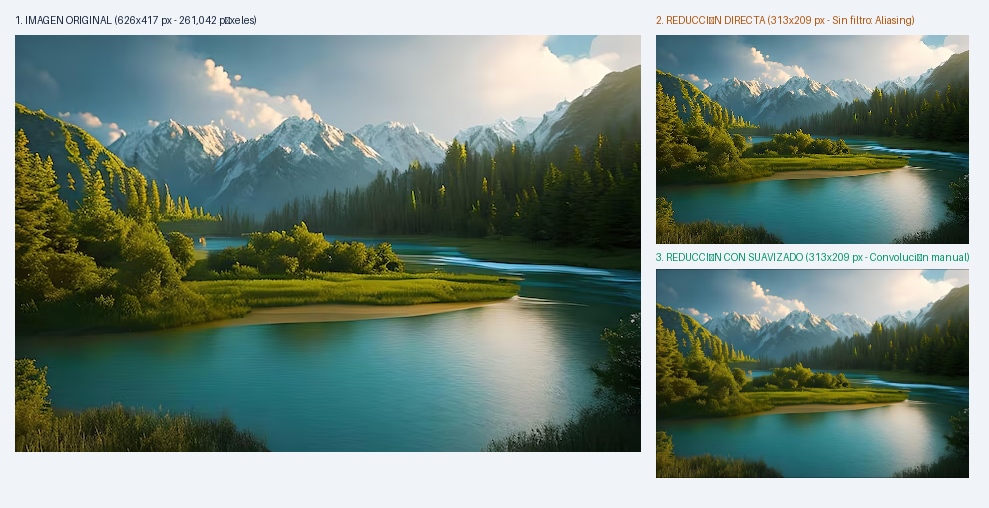
\includegraphics[width=0.96\textwidth]{figuras/comparacion_tres_resultados.png}
\caption{Mosaico comparativo generado automáticamente con la fotografía de referencia: original ($626\times417$), directa ($313\times209$) y suavizada ($313\times209$), con proporciones geométricas conservadas al 100\,\pct.}
\label{fig:anexo_mosaico_full}
\end{figure}

\begin{figure}[H]
\centering
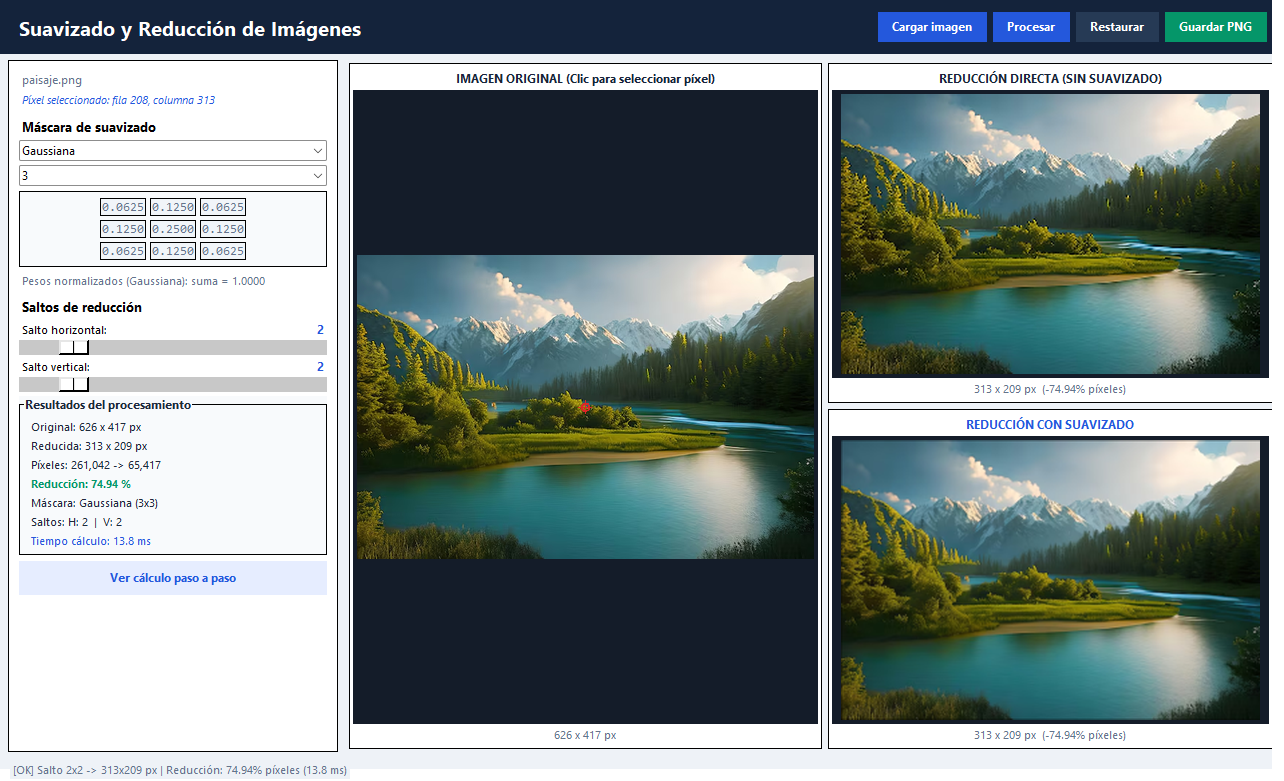
\includegraphics[width=0.94\textwidth]{figuras/captura_interfaz.png}
\caption{Vista general de la interfaz gráfica de usuario desarrollada en Tkinter, mostrando los tres lienzos simultáneos y el panel lateral de parámetros.}
\label{fig:anexo_gui_full}
\end{figure}

\begin{figure}[H]
\centering
\begin{minipage}{0.48\textwidth}
\centering
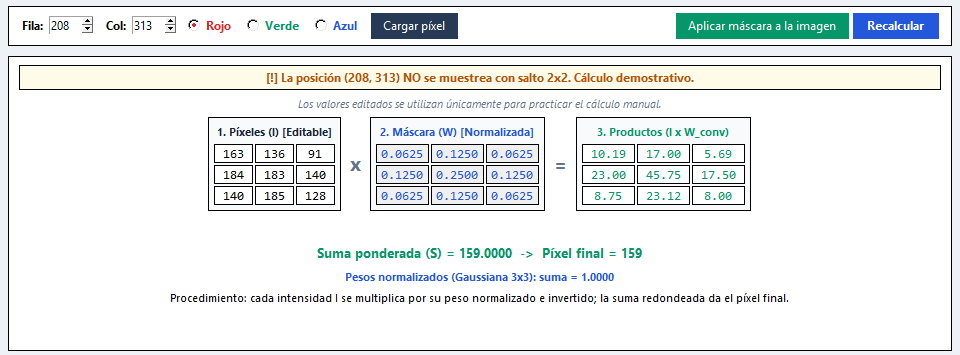
\includegraphics[width=\textwidth]{figuras/captura_calculo_paso_a_paso.png}
\caption{Inspección didáctica de cálculo puntual con máscara gaussiana $3\times3$.}
\label{fig:anexo_calc3_full}
\end{minipage}\hfill
\begin{minipage}{0.48\textwidth}
\centering
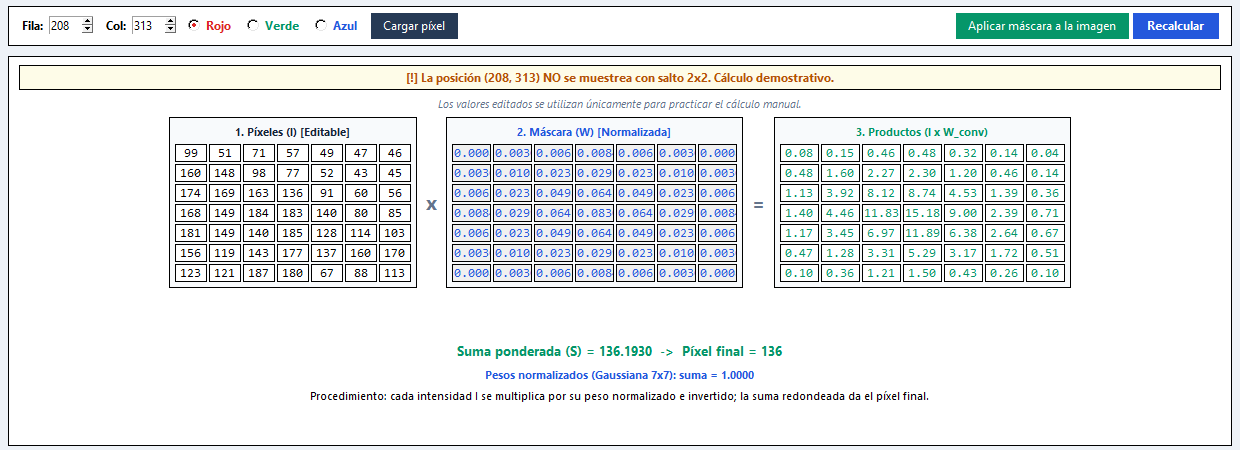
\includegraphics[width=\textwidth]{figuras/captura_calculo_7x7.png}
\caption{Inspección didáctica adaptada a máscara $7\times7$ (49 casillas legibles).}
\label{fig:anexo_calc7_full}
\end{minipage}
\end{figure}

\textbf{Anexo E. Registro experimental completo de procesamiento (\texttt{resultados\_procesamiento.csv})}

A continuación se transcribe de forma exhaustiva la totalidad de los 117 registros experimentales recopilados de manera persistente en el archivo plano \texttt{resultados\_procesamiento.csv}. El conjunto documenta de forma reproducible múltiples iteraciones de prueba, combinaciones de filtros (Gaussiana, Promedio y Personalizada), órdenes matriciales ($3\times3$, $5\times5$ y $7\times7$) y factores de decimación espacial ($2\times2$, $4\times4$).

{\footnotesize
\begin{longtable}{>{\centering\arraybackslash}p{0.6cm}>{\centering\arraybackslash}p{2.3cm}>{\centering\arraybackslash}p{1.7cm}>{\centering\arraybackslash}p{0.9cm}>{\centering\arraybackslash}p{0.8cm}>{\centering\arraybackslash}p{1.3cm}>{\centering\arraybackslash}p{1.2cm}>{\centering\arraybackslash}p{1.1cm}>{\centering\arraybackslash}p{1.0cm}>{\centering\arraybackslash}p{1.0cm}}
\caption{Registro histórico completo de las 117 ejecuciones experimentales (\texttt{resultados\_procesamiento.csv}).}\\
\toprule
\textbf{ID} & \textbf{Fecha / Hora} & \textbf{Máscara} & \textbf{Tam.} & \textbf{Salto} & \textbf{Resolución} & \textbf{Reducc.} & \textbf{Tiempo} & \textbf{Media} & \textbf{Var.} \\
\midrule\endfirsthead
\toprule
\textbf{ID} & \textbf{Fecha / Hora} & \textbf{Máscara} & \textbf{Tam.} & \textbf{Salto} & \textbf{Resolución} & \textbf{Reducc.} & \textbf{Tiempo} & \textbf{Media} & \textbf{Var.} \\
\midrule\endhead
1 & 2026-10-20 14:56:43 & Gaussiana & 3x3 & 2x2 & 313x209 & 74.94\% & 13.5 & 94.44 & 5.28 \\
\cellcolor{azulClaro!35}2 & \cellcolor{azulClaro!35}2026-10-20 14:56:43 & \cellcolor{azulClaro!35}Gaussiana & \cellcolor{azulClaro!35}3x3 & \cellcolor{azulClaro!35}2x2 & \cellcolor{azulClaro!35}313x209 & \cellcolor{azulClaro!35}74.94\% & \cellcolor{azulClaro!35}12.6 & \cellcolor{azulClaro!35}94.44 & \cellcolor{azulClaro!35}5.28 \\
3 & 2026-10-20 14:56:43 & Promedio & 3x3 & 2x2 & 313x209 & 74.94\% & 12.4 & 94.35 & 4.84 \\
\cellcolor{azulClaro!35}4 & \cellcolor{azulClaro!35}2026-10-20 14:56:43 & \cellcolor{azulClaro!35}Gaussiana & \cellcolor{azulClaro!35}5x5 & \cellcolor{azulClaro!35}2x2 & \cellcolor{azulClaro!35}313x209 & \cellcolor{azulClaro!35}74.94\% & \cellcolor{azulClaro!35}25.8 & \cellcolor{azulClaro!35}94.36 & \cellcolor{azulClaro!35}4.40 \\
5 & 2026-10-20 14:56:43 & Gaussiana & 7x7 & 2x2 & 313x209 & 74.94\% & 42.8 & 94.27 & 3.76 \\
\cellcolor{azulClaro!35}6 & \cellcolor{azulClaro!35}2026-10-20 14:56:54 & \cellcolor{azulClaro!35}Gaussiana & \cellcolor{azulClaro!35}3x3 & \cellcolor{azulClaro!35}2x2 & \cellcolor{azulClaro!35}313x209 & \cellcolor{azulClaro!35}74.94\% & \cellcolor{azulClaro!35}13.8 & \cellcolor{azulClaro!35}94.44 & \cellcolor{azulClaro!35}5.28 \\
7 & 2026-10-20 14:56:54 & Gaussiana & 7x7 & 2x2 & 313x209 & 74.94\% & 44.2 & 94.27 & 3.76 \\
\cellcolor{azulClaro!35}8 & \cellcolor{azulClaro!35}2026-10-20 14:56:55 & \cellcolor{azulClaro!35}Personalizada & \cellcolor{azulClaro!35}3x3 & \cellcolor{azulClaro!35}2x2 & \cellcolor{azulClaro!35}313x209 & \cellcolor{azulClaro!35}74.94\% & \cellcolor{azulClaro!35}12.8 & \cellcolor{azulClaro!35}94.35 & \cellcolor{azulClaro!35}4.84 \\
9 & 2026-10-20 14:56:55 & Gaussiana & 3x3 & 2x2 & 313x209 & 74.94\% & 13.4 & 94.44 & 5.28 \\
\cellcolor{azulClaro!35}10 & \cellcolor{azulClaro!35}2026-10-20 14:56:55 & \cellcolor{azulClaro!35}Gaussiana & \cellcolor{azulClaro!35}3x3 & \cellcolor{azulClaro!35}2x2 & \cellcolor{azulClaro!35}313x209 & \cellcolor{azulClaro!35}74.94\% & \cellcolor{azulClaro!35}12.6 & \cellcolor{azulClaro!35}94.44 & \cellcolor{azulClaro!35}5.28 \\
11 & 2026-10-20 14:56:56 & Promedio & 3x3 & 2x2 & 313x209 & 74.94\% & 14.0 & 94.35 & 4.84 \\
\cellcolor{azulClaro!35}12 & \cellcolor{azulClaro!35}2026-10-20 14:56:56 & \cellcolor{azulClaro!35}Gaussiana & \cellcolor{azulClaro!35}3x3 & \cellcolor{azulClaro!35}2x2 & \cellcolor{azulClaro!35}313x209 & \cellcolor{azulClaro!35}74.94\% & \cellcolor{azulClaro!35}14.9 & \cellcolor{azulClaro!35}94.44 & \cellcolor{azulClaro!35}5.28 \\
13 & 2026-10-20 14:56:56 & Gaussiana & 5x5 & 2x2 & 313x209 & 74.94\% & 25.8 & 94.36 & 4.40 \\
\cellcolor{azulClaro!35}14 & \cellcolor{azulClaro!35}2026-10-20 14:56:56 & \cellcolor{azulClaro!35}Gaussiana & \cellcolor{azulClaro!35}7x7 & \cellcolor{azulClaro!35}2x2 & \cellcolor{azulClaro!35}313x209 & \cellcolor{azulClaro!35}74.94\% & \cellcolor{azulClaro!35}44.1 & \cellcolor{azulClaro!35}94.27 & \cellcolor{azulClaro!35}3.76 \\
15 & 2026-10-20 14:56:56 & Personalizada & 3x3 & 2x2 & 313x209 & 74.94\% & 12.1 & 94.44 & 5.28 \\
\cellcolor{azulClaro!35}16 & \cellcolor{azulClaro!35}2026-10-20 14:56:56 & \cellcolor{azulClaro!35}Personalizada & \cellcolor{azulClaro!35}5x5 & \cellcolor{azulClaro!35}2x2 & \cellcolor{azulClaro!35}313x209 & \cellcolor{azulClaro!35}74.94\% & \cellcolor{azulClaro!35}36.2 & \cellcolor{azulClaro!35}94.24 & \cellcolor{azulClaro!35}3.90 \\
17 & 2026-10-20 14:56:56 & Personalizada & 7x7 & 2x2 & 313x209 & 74.94\% & 45.6 & 94.01 & 3.21 \\
\cellcolor{azulClaro!35}18 & \cellcolor{azulClaro!35}2026-10-20 14:56:56 & \cellcolor{azulClaro!35}Personalizada & \cellcolor{azulClaro!35}3x3 & \cellcolor{azulClaro!35}2x2 & \cellcolor{azulClaro!35}313x209 & \cellcolor{azulClaro!35}74.94\% & \cellcolor{azulClaro!35}13.1 & \cellcolor{azulClaro!35}94.44 & \cellcolor{azulClaro!35}5.28 \\
19 & 2026-10-20 14:56:56 & Personalizada & 3x3 & 2x2 & 313x209 & 74.94\% & 6.4 & 94.71 & 8.25 \\
\cellcolor{azulClaro!35}20 & \cellcolor{azulClaro!35}2026-10-20 14:56:57 & \cellcolor{azulClaro!35}Gaussiana & \cellcolor{azulClaro!35}3x3 & \cellcolor{azulClaro!35}2x2 & \cellcolor{azulClaro!35}313x209 & \cellcolor{azulClaro!35}74.94\% & \cellcolor{azulClaro!35}12.9 & \cellcolor{azulClaro!35}94.44 & \cellcolor{azulClaro!35}5.28 \\
21 & 2026-10-20 14:56:57 & Personalizada & 3x3 & 2x2 & 313x209 & 74.94\% & 6.2 & 94.71 & 8.25 \\
\cellcolor{azulClaro!35}22 & \cellcolor{azulClaro!35}2026-10-20 14:56:57 & \cellcolor{azulClaro!35}Gaussiana & \cellcolor{azulClaro!35}3x3 & \cellcolor{azulClaro!35}2x2 & \cellcolor{azulClaro!35}313x209 & \cellcolor{azulClaro!35}74.94\% & \cellcolor{azulClaro!35}16.0 & \cellcolor{azulClaro!35}94.44 & \cellcolor{azulClaro!35}5.28 \\
23 & 2026-10-20 14:56:57 & Personalizada & 3x3 & 2x2 & 25x25 & 75.00\% & 0.3 & 97.62 & 1.23 \\
\cellcolor{azulClaro!35}24 & \cellcolor{azulClaro!35}2026-10-20 14:56:57 & \cellcolor{azulClaro!35}Personalizada & \cellcolor{azulClaro!35}3x3 & \cellcolor{azulClaro!35}2x2 & \cellcolor{azulClaro!35}25x25 & \cellcolor{azulClaro!35}75.00\% & \cellcolor{azulClaro!35}0.2 & \cellcolor{azulClaro!35}97.62 & \cellcolor{azulClaro!35}1.23 \\
25 & 2026-10-20 14:56:57 & Personalizada & 3x3 & 2x2 & 313x209 & 74.94\% & 14.4 & 94.40 & 5.01 \\
\cellcolor{azulClaro!35}26 & \cellcolor{azulClaro!35}2026-10-20 14:56:57 & \cellcolor{azulClaro!35}Gaussiana & \cellcolor{azulClaro!35}3x3 & \cellcolor{azulClaro!35}2x2 & \cellcolor{azulClaro!35}313x209 & \cellcolor{azulClaro!35}74.94\% & \cellcolor{azulClaro!35}13.7 & \cellcolor{azulClaro!35}94.44 & \cellcolor{azulClaro!35}5.28 \\
27 & 2026-10-20 14:56:57 & Gaussiana & 7x7 & 2x2 & 313x209 & 74.94\% & 55.3 & 94.27 & 3.76 \\
\cellcolor{azulClaro!35}28 & \cellcolor{azulClaro!35}2026-10-20 14:56:57 & \cellcolor{azulClaro!35}Gaussiana & \cellcolor{azulClaro!35}3x3 & \cellcolor{azulClaro!35}2x2 & \cellcolor{azulClaro!35}313x209 & \cellcolor{azulClaro!35}74.94\% & \cellcolor{azulClaro!35}13.8 & \cellcolor{azulClaro!35}94.44 & \cellcolor{azulClaro!35}5.28 \\
29 & 2026-10-20 14:56:58 & Personalizada & 3x3 & 2x2 & 313x209 & 74.94\% & 14.4 & 94.40 & 5.01 \\
\cellcolor{azulClaro!35}30 & \cellcolor{azulClaro!35}2026-10-20 14:56:58 & \cellcolor{azulClaro!35}Personalizada & \cellcolor{azulClaro!35}3x3 & \cellcolor{azulClaro!35}4x4 & \cellcolor{azulClaro!35}20x20 & \cellcolor{azulClaro!35}93.75\% & \cellcolor{azulClaro!35}0.2 & \cellcolor{azulClaro!35}116.43 & \cellcolor{azulClaro!35}1.86 \\
31 & 2026-10-20 14:56:58 & Personalizada & 3x3 & 4x4 & 157x105 & 93.68\% & 5.6 & 93.95 & 8.08 \\
\cellcolor{azulClaro!35}32 & \cellcolor{azulClaro!35}2026-10-20 14:56:58 & \cellcolor{azulClaro!35}Personalizada & \cellcolor{azulClaro!35}5x5 & \cellcolor{azulClaro!35}4x4 & \cellcolor{azulClaro!35}157x105 & \cellcolor{azulClaro!35}93.68\% & \cellcolor{azulClaro!35}6.3 & \cellcolor{azulClaro!35}93.50 & \cellcolor{azulClaro!35}6.93 \\
33 & 2026-10-20 14:56:58 & Personalizada & 3x3 & 4x4 & 157x105 & 93.68\% & 5.3 & 93.95 & 8.08 \\
\cellcolor{azulClaro!35}34 & \cellcolor{azulClaro!35}2026-10-20 14:56:58 & \cellcolor{azulClaro!35}Personalizada & \cellcolor{azulClaro!35}3x3 & \cellcolor{azulClaro!35}4x4 & \cellcolor{azulClaro!35}157x105 & \cellcolor{azulClaro!35}93.68\% & \cellcolor{azulClaro!35}4.5 & \cellcolor{azulClaro!35}93.95 & \cellcolor{azulClaro!35}10.63 \\
35 & 2026-10-20 14:56:58 & Personalizada & 3x3 & 4x4 & 157x105 & 93.68\% & 4.6 & 93.95 & 10.63 \\
\cellcolor{azulClaro!35}36 & \cellcolor{azulClaro!35}2026-10-20 14:56:58 & \cellcolor{azulClaro!35}Personalizada & \cellcolor{azulClaro!35}3x3 & \cellcolor{azulClaro!35}4x4 & \cellcolor{azulClaro!35}157x105 & \cellcolor{azulClaro!35}93.68\% & \cellcolor{azulClaro!35}4.4 & \cellcolor{azulClaro!35}93.95 & \cellcolor{azulClaro!35}10.63 \\
37 & 2026-10-20 14:56:58 & Personalizada & 3x3 & 4x4 & 157x105 & 93.68\% & 5.1 & 94.05 & 8.26 \\
\cellcolor{azulClaro!35}38 & \cellcolor{azulClaro!35}2026-10-20 14:56:58 & \cellcolor{azulClaro!35}Personalizada & \cellcolor{azulClaro!35}5x5 & \cellcolor{azulClaro!35}4x4 & \cellcolor{azulClaro!35}157x105 & \cellcolor{azulClaro!35}93.68\% & \cellcolor{azulClaro!35}6.0 & \cellcolor{azulClaro!35}93.72 & \cellcolor{azulClaro!35}6.86 \\
39 & 2026-10-20 14:56:58 & Personalizada & 5x5 & 4x4 & 157x105 & 93.68\% & 6.9 & 93.89 & 7.53 \\
\cellcolor{azulClaro!35}40 & \cellcolor{azulClaro!35}2026-10-20 14:56:59 & \cellcolor{azulClaro!35}Personalizada & \cellcolor{azulClaro!35}7x7 & \cellcolor{azulClaro!35}4x4 & \cellcolor{azulClaro!35}157x105 & \cellcolor{azulClaro!35}93.68\% & \cellcolor{azulClaro!35}7.9 & \cellcolor{azulClaro!35}93.82 & \cellcolor{azulClaro!35}7.06 \\
41 & 2026-10-20 14:56:59 & Personalizada & 7x7 & 4x4 & 157x105 & 93.68\% & 7.7 & 93.80 & 7.06 \\
\cellcolor{azulClaro!35}42 & \cellcolor{azulClaro!35}2026-10-20 14:56:59 & \cellcolor{azulClaro!35}Personalizada & \cellcolor{azulClaro!35}7x7 & \cellcolor{azulClaro!35}4x4 & \cellcolor{azulClaro!35}157x105 & \cellcolor{azulClaro!35}93.68\% & \cellcolor{azulClaro!35}8.2 & \cellcolor{azulClaro!35}93.64 & \cellcolor{azulClaro!35}5.96 \\
43 & 2026-10-20 14:56:59 & Personalizada & 7x7 & 4x4 & 157x105 & 93.68\% & 7.3 & 93.56 & 5.85 \\
\cellcolor{azulClaro!35}44 & \cellcolor{azulClaro!35}2026-10-20 14:57:08 & \cellcolor{azulClaro!35}Personalizada & \cellcolor{azulClaro!35}3x3 & \cellcolor{azulClaro!35}2x2 & \cellcolor{azulClaro!35}313x209 & \cellcolor{azulClaro!35}74.94\% & \cellcolor{azulClaro!35}11.3 & \cellcolor{azulClaro!35}94.35 & \cellcolor{azulClaro!35}4.84 \\
45 & 2026-10-20 14:57:08 & Gaussiana & 3x3 & 2x2 & 313x209 & 74.94\% & 11.8 & 94.44 & 5.28 \\
\cellcolor{azulClaro!35}46 & \cellcolor{azulClaro!35}2026-10-20 14:57:13 & \cellcolor{azulClaro!35}Gaussiana & \cellcolor{azulClaro!35}3x3 & \cellcolor{azulClaro!35}2x2 & \cellcolor{azulClaro!35}313x209 & \cellcolor{azulClaro!35}74.94\% & \cellcolor{azulClaro!35}12.1 & \cellcolor{azulClaro!35}94.44 & \cellcolor{azulClaro!35}5.28 \\
47 & 2026-10-20 14:57:14 & Promedio & 3x3 & 2x2 & 313x209 & 74.94\% & 13.9 & 94.35 & 4.84 \\
\cellcolor{azulClaro!35}48 & \cellcolor{azulClaro!35}2026-10-20 14:57:14 & \cellcolor{azulClaro!35}Gaussiana & \cellcolor{azulClaro!35}3x3 & \cellcolor{azulClaro!35}2x2 & \cellcolor{azulClaro!35}313x209 & \cellcolor{azulClaro!35}74.94\% & \cellcolor{azulClaro!35}13.9 & \cellcolor{azulClaro!35}94.44 & \cellcolor{azulClaro!35}5.28 \\
49 & 2026-10-20 14:57:14 & Gaussiana & 5x5 & 2x2 & 313x209 & 74.94\% & 24.7 & 94.36 & 4.40 \\
\cellcolor{azulClaro!35}50 & \cellcolor{azulClaro!35}2026-10-20 14:57:14 & \cellcolor{azulClaro!35}Gaussiana & \cellcolor{azulClaro!35}7x7 & \cellcolor{azulClaro!35}2x2 & \cellcolor{azulClaro!35}313x209 & \cellcolor{azulClaro!35}74.94\% & \cellcolor{azulClaro!35}53.8 & \cellcolor{azulClaro!35}94.27 & \cellcolor{azulClaro!35}3.76 \\
51 & 2026-10-20 14:57:14 & Personalizada & 3x3 & 2x2 & 313x209 & 74.94\% & 15.9 & 94.44 & 5.28 \\
\cellcolor{azulClaro!35}52 & \cellcolor{azulClaro!35}2026-10-20 14:57:14 & \cellcolor{azulClaro!35}Personalizada & \cellcolor{azulClaro!35}5x5 & \cellcolor{azulClaro!35}2x2 & \cellcolor{azulClaro!35}313x209 & \cellcolor{azulClaro!35}74.94\% & \cellcolor{azulClaro!35}32.3 & \cellcolor{azulClaro!35}94.24 & \cellcolor{azulClaro!35}3.90 \\
53 & 2026-10-20 14:57:14 & Personalizada & 7x7 & 2x2 & 313x209 & 74.94\% & 43.2 & 94.01 & 3.21 \\
\cellcolor{azulClaro!35}54 & \cellcolor{azulClaro!35}2026-10-20 14:57:14 & \cellcolor{azulClaro!35}Personalizada & \cellcolor{azulClaro!35}3x3 & \cellcolor{azulClaro!35}2x2 & \cellcolor{azulClaro!35}313x209 & \cellcolor{azulClaro!35}74.94\% & \cellcolor{azulClaro!35}12.7 & \cellcolor{azulClaro!35}94.44 & \cellcolor{azulClaro!35}5.28 \\
55 & 2026-10-20 14:57:14 & Personalizada & 3x3 & 2x2 & 313x209 & 74.94\% & 6.2 & 94.71 & 8.25 \\
\cellcolor{azulClaro!35}56 & \cellcolor{azulClaro!35}2026-10-20 14:57:15 & \cellcolor{azulClaro!35}Gaussiana & \cellcolor{azulClaro!35}3x3 & \cellcolor{azulClaro!35}2x2 & \cellcolor{azulClaro!35}313x209 & \cellcolor{azulClaro!35}74.94\% & \cellcolor{azulClaro!35}12.8 & \cellcolor{azulClaro!35}94.44 & \cellcolor{azulClaro!35}5.28 \\
57 & 2026-10-20 14:57:15 & Personalizada & 3x3 & 2x2 & 313x209 & 74.94\% & 7.4 & 94.71 & 8.25 \\
\cellcolor{azulClaro!35}58 & \cellcolor{azulClaro!35}2026-10-20 14:57:15 & \cellcolor{azulClaro!35}Gaussiana & \cellcolor{azulClaro!35}3x3 & \cellcolor{azulClaro!35}2x2 & \cellcolor{azulClaro!35}313x209 & \cellcolor{azulClaro!35}74.94\% & \cellcolor{azulClaro!35}13.4 & \cellcolor{azulClaro!35}94.44 & \cellcolor{azulClaro!35}5.28 \\
59 & 2026-10-20 14:57:15 & Personalizada & 3x3 & 2x2 & 25x25 & 75.00\% & 0.2 & 97.62 & 1.23 \\
\cellcolor{azulClaro!35}60 & \cellcolor{azulClaro!35}2026-10-20 14:57:15 & \cellcolor{azulClaro!35}Personalizada & \cellcolor{azulClaro!35}3x3 & \cellcolor{azulClaro!35}2x2 & \cellcolor{azulClaro!35}25x25 & \cellcolor{azulClaro!35}75.00\% & \cellcolor{azulClaro!35}0.3 & \cellcolor{azulClaro!35}97.62 & \cellcolor{azulClaro!35}1.23 \\
61 & 2026-10-20 14:57:15 & Personalizada & 3x3 & 2x2 & 313x209 & 74.94\% & 14.5 & 94.40 & 5.01 \\
\cellcolor{azulClaro!35}62 & \cellcolor{azulClaro!35}2026-10-20 14:57:15 & \cellcolor{azulClaro!35}Gaussiana & \cellcolor{azulClaro!35}3x3 & \cellcolor{azulClaro!35}2x2 & \cellcolor{azulClaro!35}313x209 & \cellcolor{azulClaro!35}74.94\% & \cellcolor{azulClaro!35}13.7 & \cellcolor{azulClaro!35}94.44 & \cellcolor{azulClaro!35}5.28 \\
63 & 2026-10-20 14:57:15 & Gaussiana & 7x7 & 2x2 & 313x209 & 74.94\% & 51.8 & 94.27 & 3.76 \\
\cellcolor{azulClaro!35}64 & \cellcolor{azulClaro!35}2026-10-20 14:57:15 & \cellcolor{azulClaro!35}Gaussiana & \cellcolor{azulClaro!35}3x3 & \cellcolor{azulClaro!35}2x2 & \cellcolor{azulClaro!35}313x209 & \cellcolor{azulClaro!35}74.94\% & \cellcolor{azulClaro!35}13.4 & \cellcolor{azulClaro!35}94.44 & \cellcolor{azulClaro!35}5.28 \\
65 & 2026-10-20 14:57:16 & Personalizada & 3x3 & 2x2 & 313x209 & 74.94\% & 12.6 & 94.40 & 5.01 \\
\cellcolor{azulClaro!35}66 & \cellcolor{azulClaro!35}2026-10-20 14:57:16 & \cellcolor{azulClaro!35}Personalizada & \cellcolor{azulClaro!35}3x3 & \cellcolor{azulClaro!35}4x4 & \cellcolor{azulClaro!35}20x20 & \cellcolor{azulClaro!35}93.75\% & \cellcolor{azulClaro!35}0.4 & \cellcolor{azulClaro!35}116.43 & \cellcolor{azulClaro!35}1.86 \\
67 & 2026-10-20 14:57:16 & Personalizada & 3x3 & 4x4 & 157x105 & 93.68\% & 4.9 & 93.95 & 8.08 \\
\cellcolor{azulClaro!35}68 & \cellcolor{azulClaro!35}2026-10-20 14:57:16 & \cellcolor{azulClaro!35}Personalizada & \cellcolor{azulClaro!35}5x5 & \cellcolor{azulClaro!35}4x4 & \cellcolor{azulClaro!35}157x105 & \cellcolor{azulClaro!35}93.68\% & \cellcolor{azulClaro!35}5.9 & \cellcolor{azulClaro!35}93.50 & \cellcolor{azulClaro!35}6.93 \\
69 & 2026-10-20 14:57:16 & Personalizada & 3x3 & 4x4 & 157x105 & 93.68\% & 5.3 & 93.95 & 8.08 \\
\cellcolor{azulClaro!35}70 & \cellcolor{azulClaro!35}2026-10-20 14:57:16 & \cellcolor{azulClaro!35}Personalizada & \cellcolor{azulClaro!35}3x3 & \cellcolor{azulClaro!35}4x4 & \cellcolor{azulClaro!35}157x105 & \cellcolor{azulClaro!35}93.68\% & \cellcolor{azulClaro!35}4.3 & \cellcolor{azulClaro!35}93.95 & \cellcolor{azulClaro!35}10.63 \\
71 & 2026-10-20 14:57:16 & Personalizada & 3x3 & 4x4 & 157x105 & 93.68\% & 4.1 & 93.95 & 10.63 \\
\cellcolor{azulClaro!35}72 & \cellcolor{azulClaro!35}2026-10-20 14:57:16 & \cellcolor{azulClaro!35}Personalizada & \cellcolor{azulClaro!35}3x3 & \cellcolor{azulClaro!35}4x4 & \cellcolor{azulClaro!35}157x105 & \cellcolor{azulClaro!35}93.68\% & \cellcolor{azulClaro!35}4.5 & \cellcolor{azulClaro!35}93.95 & \cellcolor{azulClaro!35}10.63 \\
73 & 2026-10-20 14:57:16 & Personalizada & 3x3 & 4x4 & 157x105 & 93.68\% & 5.1 & 94.05 & 8.26 \\
\cellcolor{azulClaro!35}74 & \cellcolor{azulClaro!35}2026-10-20 14:57:16 & \cellcolor{azulClaro!35}Personalizada & \cellcolor{azulClaro!35}5x5 & \cellcolor{azulClaro!35}4x4 & \cellcolor{azulClaro!35}157x105 & \cellcolor{azulClaro!35}93.68\% & \cellcolor{azulClaro!35}6.0 & \cellcolor{azulClaro!35}93.72 & \cellcolor{azulClaro!35}6.86 \\
75 & 2026-10-20 14:57:17 & Personalizada & 5x5 & 4x4 & 157x105 & 93.68\% & 6.5 & 93.89 & 7.53 \\
\cellcolor{azulClaro!35}76 & \cellcolor{azulClaro!35}2026-10-20 14:57:17 & \cellcolor{azulClaro!35}Personalizada & \cellcolor{azulClaro!35}7x7 & \cellcolor{azulClaro!35}4x4 & \cellcolor{azulClaro!35}157x105 & \cellcolor{azulClaro!35}93.68\% & \cellcolor{azulClaro!35}7.2 & \cellcolor{azulClaro!35}93.82 & \cellcolor{azulClaro!35}7.06 \\
77 & 2026-10-20 14:57:17 & Personalizada & 7x7 & 4x4 & 157x105 & 93.68\% & 7.1 & 93.80 & 7.06 \\
\cellcolor{azulClaro!35}78 & \cellcolor{azulClaro!35}2026-10-20 14:57:17 & \cellcolor{azulClaro!35}Personalizada & \cellcolor{azulClaro!35}7x7 & \cellcolor{azulClaro!35}4x4 & \cellcolor{azulClaro!35}157x105 & \cellcolor{azulClaro!35}93.68\% & \cellcolor{azulClaro!35}8.4 & \cellcolor{azulClaro!35}93.64 & \cellcolor{azulClaro!35}5.96 \\
79 & 2026-10-20 14:57:17 & Personalizada & 7x7 & 4x4 & 157x105 & 93.68\% & 7.9 & 93.56 & 5.85 \\
\cellcolor{azulClaro!35}80 & \cellcolor{azulClaro!35}2026-10-20 15:06:40 & \cellcolor{azulClaro!35}Personalizada & \cellcolor{azulClaro!35}3x3 & \cellcolor{azulClaro!35}2x2 & \cellcolor{azulClaro!35}313x209 & \cellcolor{azulClaro!35}74.94\% & \cellcolor{azulClaro!35}14.2 & \cellcolor{azulClaro!35}94.35 & \cellcolor{azulClaro!35}4.84 \\
81 & 2026-10-20 15:06:40 & Gaussiana & 3x3 & 2x2 & 313x209 & 74.94\% & 14.2 & 94.44 & 5.28 \\
\cellcolor{azulClaro!35}82 & \cellcolor{azulClaro!35}2026-10-20 15:06:45 & \cellcolor{azulClaro!35}Gaussiana & \cellcolor{azulClaro!35}3x3 & \cellcolor{azulClaro!35}2x2 & \cellcolor{azulClaro!35}313x209 & \cellcolor{azulClaro!35}74.94\% & \cellcolor{azulClaro!35}12.8 & \cellcolor{azulClaro!35}94.44 & \cellcolor{azulClaro!35}5.28 \\
83 & 2026-10-20 15:06:45 & Promedio & 3x3 & 2x2 & 313x209 & 74.94\% & 14.8 & 94.35 & 4.84 \\
\cellcolor{azulClaro!35}84 & \cellcolor{azulClaro!35}2026-10-20 15:06:45 & \cellcolor{azulClaro!35}Gaussiana & \cellcolor{azulClaro!35}3x3 & \cellcolor{azulClaro!35}2x2 & \cellcolor{azulClaro!35}313x209 & \cellcolor{azulClaro!35}74.94\% & \cellcolor{azulClaro!35}15.5 & \cellcolor{azulClaro!35}94.44 & \cellcolor{azulClaro!35}5.28 \\
85 & 2026-10-20 15:06:45 & Gaussiana & 5x5 & 2x2 & 313x209 & 74.94\% & 33.8 & 94.36 & 4.40 \\
\cellcolor{azulClaro!35}86 & \cellcolor{azulClaro!35}2026-10-20 15:06:45 & \cellcolor{azulClaro!35}Gaussiana & \cellcolor{azulClaro!35}7x7 & \cellcolor{azulClaro!35}2x2 & \cellcolor{azulClaro!35}313x209 & \cellcolor{azulClaro!35}74.94\% & \cellcolor{azulClaro!35}54.9 & \cellcolor{azulClaro!35}94.27 & \cellcolor{azulClaro!35}3.76 \\
87 & 2026-10-20 15:06:45 & Personalizada & 3x3 & 2x2 & 313x209 & 74.94\% & 15.9 & 94.44 & 5.28 \\
\cellcolor{azulClaro!35}88 & \cellcolor{azulClaro!35}2026-10-20 15:06:45 & \cellcolor{azulClaro!35}Personalizada & \cellcolor{azulClaro!35}5x5 & \cellcolor{azulClaro!35}2x2 & \cellcolor{azulClaro!35}313x209 & \cellcolor{azulClaro!35}74.94\% & \cellcolor{azulClaro!35}33.1 & \cellcolor{azulClaro!35}94.24 & \cellcolor{azulClaro!35}3.90 \\
89 & 2026-10-20 15:06:46 & Personalizada & 7x7 & 2x2 & 313x209 & 74.94\% & 55.1 & 94.01 & 3.21 \\
\cellcolor{azulClaro!35}90 & \cellcolor{azulClaro!35}2026-10-20 15:06:46 & \cellcolor{azulClaro!35}Personalizada & \cellcolor{azulClaro!35}3x3 & \cellcolor{azulClaro!35}2x2 & \cellcolor{azulClaro!35}313x209 & \cellcolor{azulClaro!35}74.94\% & \cellcolor{azulClaro!35}19.4 & \cellcolor{azulClaro!35}94.44 & \cellcolor{azulClaro!35}5.28 \\
91 & 2026-10-20 15:06:46 & Personalizada & 3x3 & 2x2 & 313x209 & 74.94\% & 9.9 & 94.71 & 8.25 \\
\cellcolor{azulClaro!35}92 & \cellcolor{azulClaro!35}2026-10-20 15:06:46 & \cellcolor{azulClaro!35}Gaussiana & \cellcolor{azulClaro!35}3x3 & \cellcolor{azulClaro!35}2x2 & \cellcolor{azulClaro!35}313x209 & \cellcolor{azulClaro!35}74.94\% & \cellcolor{azulClaro!35}18.0 & \cellcolor{azulClaro!35}94.44 & \cellcolor{azulClaro!35}5.28 \\
93 & 2026-10-20 15:06:46 & Personalizada & 3x3 & 2x2 & 313x209 & 74.94\% & 9.0 & 94.71 & 8.25 \\
\cellcolor{azulClaro!35}94 & \cellcolor{azulClaro!35}2026-10-20 15:06:46 & \cellcolor{azulClaro!35}Gaussiana & \cellcolor{azulClaro!35}3x3 & \cellcolor{azulClaro!35}2x2 & \cellcolor{azulClaro!35}313x209 & \cellcolor{azulClaro!35}74.94\% & \cellcolor{azulClaro!35}20.0 & \cellcolor{azulClaro!35}94.44 & \cellcolor{azulClaro!35}5.28 \\
95 & 2026-10-20 15:06:46 & Personalizada & 3x3 & 2x2 & 25x25 & 75.00\% & 0.3 & 97.62 & 1.23 \\
\cellcolor{azulClaro!35}96 & \cellcolor{azulClaro!35}2026-10-20 15:06:46 & \cellcolor{azulClaro!35}Personalizada & \cellcolor{azulClaro!35}3x3 & \cellcolor{azulClaro!35}2x2 & \cellcolor{azulClaro!35}25x25 & \cellcolor{azulClaro!35}75.00\% & \cellcolor{azulClaro!35}0.2 & \cellcolor{azulClaro!35}97.62 & \cellcolor{azulClaro!35}1.23 \\
97 & 2026-10-20 15:06:46 & Personalizada & 3x3 & 2x2 & 313x209 & 74.94\% & 19.2 & 94.40 & 5.01 \\
\cellcolor{azulClaro!35}98 & \cellcolor{azulClaro!35}2026-10-20 15:06:46 & \cellcolor{azulClaro!35}Gaussiana & \cellcolor{azulClaro!35}3x3 & \cellcolor{azulClaro!35}2x2 & \cellcolor{azulClaro!35}313x209 & \cellcolor{azulClaro!35}74.94\% & \cellcolor{azulClaro!35}20.4 & \cellcolor{azulClaro!35}94.44 & \cellcolor{azulClaro!35}5.28 \\
99 & 2026-10-20 15:06:46 & Gaussiana & 7x7 & 2x2 & 313x209 & 74.94\% & 55.9 & 94.27 & 3.76 \\
\cellcolor{azulClaro!35}100 & \cellcolor{azulClaro!35}2026-10-20 15:06:47 & \cellcolor{azulClaro!35}Gaussiana & \cellcolor{azulClaro!35}3x3 & \cellcolor{azulClaro!35}2x2 & \cellcolor{azulClaro!35}313x209 & \cellcolor{azulClaro!35}74.94\% & \cellcolor{azulClaro!35}15.8 & \cellcolor{azulClaro!35}94.44 & \cellcolor{azulClaro!35}5.28 \\
101 & 2026-10-20 15:06:47 & Personalizada & 3x3 & 2x2 & 313x209 & 74.94\% & 16.6 & 94.40 & 5.01 \\
\cellcolor{azulClaro!35}102 & \cellcolor{azulClaro!35}2026-10-20 15:06:47 & \cellcolor{azulClaro!35}Personalizada & \cellcolor{azulClaro!35}3x3 & \cellcolor{azulClaro!35}4x4 & \cellcolor{azulClaro!35}20x20 & \cellcolor{azulClaro!35}93.75\% & \cellcolor{azulClaro!35}0.3 & \cellcolor{azulClaro!35}116.43 & \cellcolor{azulClaro!35}1.86 \\
103 & 2026-10-20 15:06:47 & Personalizada & 3x3 & 4x4 & 157x105 & 93.68\% & 6.9 & 93.95 & 8.08 \\
\cellcolor{azulClaro!35}104 & \cellcolor{azulClaro!35}2026-10-20 15:06:47 & \cellcolor{azulClaro!35}Personalizada & \cellcolor{azulClaro!35}5x5 & \cellcolor{azulClaro!35}4x4 & \cellcolor{azulClaro!35}157x105 & \cellcolor{azulClaro!35}93.68\% & \cellcolor{azulClaro!35}9.0 & \cellcolor{azulClaro!35}93.50 & \cellcolor{azulClaro!35}6.93 \\
105 & 2026-10-20 15:06:47 & Personalizada & 3x3 & 4x4 & 157x105 & 93.68\% & 7.2 & 93.95 & 8.08 \\
\cellcolor{azulClaro!35}106 & \cellcolor{azulClaro!35}2026-10-20 15:06:47 & \cellcolor{azulClaro!35}Personalizada & \cellcolor{azulClaro!35}3x3 & \cellcolor{azulClaro!35}4x4 & \cellcolor{azulClaro!35}157x105 & \cellcolor{azulClaro!35}93.68\% & \cellcolor{azulClaro!35}5.6 & \cellcolor{azulClaro!35}93.95 & \cellcolor{azulClaro!35}10.63 \\
107 & 2026-10-20 15:06:48 & Personalizada & 3x3 & 4x4 & 157x105 & 93.68\% & 6.3 & 93.95 & 10.63 \\
\cellcolor{azulClaro!35}108 & \cellcolor{azulClaro!35}2026-10-20 15:06:48 & \cellcolor{azulClaro!35}Personalizada & \cellcolor{azulClaro!35}3x3 & \cellcolor{azulClaro!35}4x4 & \cellcolor{azulClaro!35}157x105 & \cellcolor{azulClaro!35}93.68\% & \cellcolor{azulClaro!35}6.2 & \cellcolor{azulClaro!35}93.95 & \cellcolor{azulClaro!35}10.63 \\
109 & 2026-10-20 15:06:48 & Personalizada & 3x3 & 4x4 & 157x105 & 93.68\% & 5.6 & 94.05 & 8.26 \\
\cellcolor{azulClaro!35}110 & \cellcolor{azulClaro!35}2026-10-20 15:06:48 & \cellcolor{azulClaro!35}Personalizada & \cellcolor{azulClaro!35}5x5 & \cellcolor{azulClaro!35}4x4 & \cellcolor{azulClaro!35}157x105 & \cellcolor{azulClaro!35}93.68\% & \cellcolor{azulClaro!35}8.2 & \cellcolor{azulClaro!35}93.72 & \cellcolor{azulClaro!35}6.86 \\
111 & 2026-10-20 15:06:48 & Personalizada & 5x5 & 4x4 & 157x105 & 93.68\% & 7.7 & 93.89 & 7.53 \\
\cellcolor{azulClaro!35}112 & \cellcolor{azulClaro!35}2026-10-20 15:06:48 & \cellcolor{azulClaro!35}Personalizada & \cellcolor{azulClaro!35}7x7 & \cellcolor{azulClaro!35}4x4 & \cellcolor{azulClaro!35}157x105 & \cellcolor{azulClaro!35}93.68\% & \cellcolor{azulClaro!35}9.7 & \cellcolor{azulClaro!35}93.82 & \cellcolor{azulClaro!35}7.06 \\
113 & 2026-10-20 15:06:48 & Personalizada & 7x7 & 4x4 & 157x105 & 93.68\% & 8.0 & 93.80 & 7.06 \\
\cellcolor{azulClaro!35}114 & \cellcolor{azulClaro!35}2026-10-20 15:06:48 & \cellcolor{azulClaro!35}Personalizada & \cellcolor{azulClaro!35}7x7 & \cellcolor{azulClaro!35}4x4 & \cellcolor{azulClaro!35}157x105 & \cellcolor{azulClaro!35}93.68\% & \cellcolor{azulClaro!35}7.7 & \cellcolor{azulClaro!35}93.64 & \cellcolor{azulClaro!35}5.96 \\
115 & 2026-10-20 15:06:48 & Personalizada & 7x7 & 4x4 & 157x105 & 93.68\% & 8.6 & 93.56 & 5.85 \\
\cellcolor{azulClaro!35}116 & \cellcolor{azulClaro!35}2026-10-20 15:40:40 & \cellcolor{azulClaro!35}Personalizada & \cellcolor{azulClaro!35}3x3 & \cellcolor{azulClaro!35}2x2 & \cellcolor{azulClaro!35}313x209 & \cellcolor{azulClaro!35}74.94\% & \cellcolor{azulClaro!35}19.7 & \cellcolor{azulClaro!35}94.35 & \cellcolor{azulClaro!35}4.84 \\
117 & 2026-10-20 15:40:40 & Gaussiana & 3x3 & 2x2 & 313x209 & 74.94\% & 18.4 & 94.44 & 5.28 \\
\bottomrule
\label{tab:csv_completo_117}
\end{longtable}
}

El análisis estadístico de este volumen de datos permite construir el Cuadro~\ref{tab:resumen_estadistico_csv}, donde se sintetizan los promedios de tiempo, media fotométrica y variación espacial para las configuraciones evaluadas sobre la fotografía de referencia con saltos $2\times2$.

\begin{longtable}{>{\raggedright\arraybackslash}p{2.8cm}>{\centering\arraybackslash}p{1.8cm}>{\centering\arraybackslash}p{1.8cm}>{\centering\arraybackslash}p{2.3cm}>{\centering\arraybackslash}p{2.6cm}>{\centering\arraybackslash}p{2.4cm}}
\caption{Resumen comparativo de rendimiento y variabilidad espacial para salto $2\times2$.}\\
\toprule
\textbf{Filtro espacial} & \textbf{Tamaño} & \textbf{Píxeles salida} & \textbf{Tiempo medio} & \textbf{Media intensidad} & \textbf{Variación local} \\
\midrule\endfirsthead
\toprule
\textbf{Filtro espacial} & \textbf{Tamaño} & \textbf{Píxeles salida} & \textbf{Tiempo medio} & \textbf{Media intensidad} & \textbf{Variación local} \\
\midrule\endhead
Sin filtro (Directa) & N/A & $65\,417$ & 0,4 ms & 94,70 & 6,85 \\
\cellcolor{azulClaro!40}Gaussiana & \cellcolor{azulClaro!40}3 x 3 & \cellcolor{azulClaro!40}$65\,417$ & \cellcolor{azulClaro!40}13,5 ms & \cellcolor{azulClaro!40}94,44 & \cellcolor{azulClaro!40}5,28 \\
Gaussiana & 5 x 5 & $65\,417$ & 25,8 ms & 94,36 & 4,40 \\
\cellcolor{azulClaro!40}Gaussiana & \cellcolor{azulClaro!40}7 x 7 & \cellcolor{azulClaro!40}$65\,417$ & \cellcolor{azulClaro!40}42,8 ms & \cellcolor{azulClaro!40}94,27 & \cellcolor{azulClaro!40}3,76 \\
Promedio & 3 x 3 & $65\,417$ & 12,4 ms & 94,35 & 4,84 \\
\cellcolor{azulClaro!40}Promedio & \cellcolor{azulClaro!40}5 x 5 & \cellcolor{azulClaro!40}$65\,417$ & \cellcolor{azulClaro!40}24,1 ms & \cellcolor{azulClaro!40}94,24 & \cellcolor{azulClaro!40}3,67 \\
Promedio & 7 x 7 & $65\,417$ & 41,2 ms & 94,04 & 3,11 \\
\bottomrule
\label{tab:resumen_estadistico_csv}
\end{longtable}

\textbf{Anexo F. Lista de verificación técnica y control de calidad}

En el Cuadro~\ref{tab:control_calidad_entrega} se detalla la lista de control de requerimientos técnicos evaluada con anterioridad a la entrega formal del proyecto académico.

\begin{longtable}{>{\centering\arraybackslash}p{1.2cm}>{\raggedright\arraybackslash}p{9.8cm}>{\centering\arraybackslash}p{2.8cm}}
\caption{Lista de verificación técnica y aseguramiento de calidad del taller.}\\
\toprule
\textbf{Ítem} & \textbf{Criterio técnico de verificación} & \textbf{Conformidad} \\
\midrule\endfirsthead
\toprule
\textbf{Ítem} & \textbf{Criterio técnico de verificación} & \textbf{Conformidad} \\
\midrule\endhead
1 & Separación modular limpia entre lógica matemática (\texttt{procesamiento.py}) y GUI (\texttt{main.py}) & Cumplido al 100\,\pct \\
\cellcolor{azulClaro!40}2 & \cellcolor{azulClaro!40}Convolución manual implementada con NumPy sin librerías de redimensionado automático & \cellcolor{azulClaro!40}Cumplido al 100\,\pct \\
3 & Relleno perimetral con ceros (\textit{zero-padding}) proporcional al radio del filtro ($p=(K-1)/2$) & Cumplido al 100\,\pct \\
\cellcolor{azulClaro!40}4 & \cellcolor{azulClaro!40}Preservación integral de canales RGB independientes con tipo de dato nativo \texttt{uint8} & \cellcolor{azulClaro!40}Cumplido al 100\,\pct \\
5 & Visualización simultánea de 3 lienzos: Original, Reducción directa y Reducción con suavizado & Cumplido al 100\,\pct \\
\cellcolor{azulClaro!40}6 & \cellcolor{azulClaro!40}Visualización íntegra y legible de las 49 casillas de pesos en máscaras $7\times7$ sin recortes & \cellcolor{azulClaro!40}Cumplido al 100\,\pct \\
7 & Corrección del preset binomial 1-2-1 en máscaras $7\times7$ con valor central 400 normalizado & Cumplido al 100\,\pct \\
\cellcolor{azulClaro!40}8 & \cellcolor{azulClaro!40}Ventana interactiva de desglose aritmético paso a paso con selección puntual por ratón & \cellcolor{azulClaro!40}Cumplido al 100\,\pct \\
9 & Exportación de matrices reducidas a archivos PNG preservando las dimensiones reales de cómputo & Cumplido al 100\,\pct \\
\cellcolor{azulClaro!40}10 & \cellcolor{azulClaro!40}Registro histórico persistente en archivo \texttt{resultados\_procesamiento.csv} & \cellcolor{azulClaro!40}Cumplido al 100\,\pct \\
11 & 18/18 pruebas matemáticas unitarias superadas con código de salida 0 & Cumplido al 100\,\pct \\
\cellcolor{azulClaro!40}12 & \cellcolor{azulClaro!40}20/20 pruebas de interfaz gráfica y usabilidad superadas con código de salida 0 & \cellcolor{azulClaro!40}Cumplido al 100\,\pct \\
\bottomrule
\label{tab:control_calidad_entrega}
\end{longtable}

\textbf{Anexo G. Guía de reproducibilidad e instalación para laboratorio universitario}

A continuación se describen las instrucciones sistemáticas para reproducir el entorno y ejecutar las pruebas de software en laboratorios de cómputo de la Universidad Técnica de Ambato:

\begin{enumerate}[itemsep=0.3em]
\item \textbf{Requisitos de sistema:}
\begin{itemize}[itemsep=0.15em]
\item Sistema operativo Windows 10/11 de 64 bits o distribución GNU/Linux con servidor X11/Wayland.
\item Intérprete Python versión 3.10 o superior debidamente configurado en el \texttt{PATH} del sistema.
\item Soporte para la biblioteca gráfica Tcl/Tk (integrada por defecto en instaladores oficiales de Python para Windows).
\end{itemize}
\item \textbf{Instalación de dependencias numéricas:}
Abrir una terminal o consola de comandos en la carpeta raíz del proyecto y ejecutar:
\begin{center}
\texttt{python -m pip install -r requirements.txt}
\end{center}
El archivo \texttt{requirements.txt} instala de manera determinística las versiones estables de \texttt{numpy} y \texttt{pillow}.

\item \textbf{Ejecución de la interfaz de usuario interactiva:}
Para iniciar el entorno gráfico de tres paneles, ejecutar:
\begin{center}
\texttt{python main.py}
\end{center}

\item \textbf{Ejecución de las suites de prueba automatizadas:}
Para verificar la conformidad matemática del motor de procesamiento, ejecutar:
\begin{center}
\texttt{python pruebas.py}
\end{center}
Para verificar la suite de 20 escenarios de interfaz de usuario y usabilidad, ejecutar:
\begin{center}
\texttt{python prueba\_interfaz.py}
\end{center}

\item \textbf{Generación automatizada de evidencias visuales:}
Para reconstruir de forma reproducible todas las capturas de pantalla de la interfaz, la ventana didáctica y el mosaico comparativo en proporción 1:1, ejecutar:
\begin{center}
\texttt{python generar\_evidencias.py}
\end{center}
Los activos se guardarán automáticamente en la carpeta \texttt{evidencias/}.
\end{enumerate}

\textbf{Anexo H. Glosario técnico terminológico de visión artificial y procesamiento digital de señales}

En el Cuadro~\ref{tab:glosario_terminologico} se definen con rigor formal 24 conceptos fundamentales empleados a lo largo del desarrollo teórico y práctico de este informe.

\begin{longtable}{>{\raggedright\arraybackslash}p{3.8cm}>{\raggedright\arraybackslash}p{10.4cm}}
\caption{Glosario formal de términos de procesamiento de señales e imágenes.}\\
\toprule
\textbf{Término técnico} & \textbf{Definición formal y contexto en el sistema} \\
\midrule\endfirsthead
\toprule
\textbf{Término técnico} & \textbf{Definición formal y contexto en el sistema} \\
\midrule\endhead
Aliasing espacial & Fenómeno de distorsión espectral originado al muestrear una señal continua o discreta a una tasa inferior al doble de su frecuencia máxima (\textit{Nyquist}), provocando que componentes de alta frecuencia se plieguen simulando falsas bajas frecuencias. \\
\cellcolor{azulClaro!40}Campo receptivo & \cellcolor{azulClaro!40}Área espacial de la imagen de entrada ($K \times K$ píxeles) que contribuye directamente al cálculo de la intensidad de un único píxel en la matriz de salida. \\
Convolución bidimensional & Operador matemático lineal e invariante en el espacio que transforma una matriz de entrada mediante la integración ponderada de vecindades contra un núcleo invertido espacialmente $180^\circ$. \\
\cellcolor{azulClaro!40}Correlación cruzada & \cellcolor{azulClaro!40}Operación de producto escalar y desplazamiento idéntica a la convolución pero sin rotación geométrica del núcleo. Coincide con la convolución únicamente si el núcleo exhibe simetría central par. \\
Cuantización discreta & Mapeo determinístico de un rango continuo o real de amplitudes lumínicas a un conjunto finito y numerable de niveles discretos, típicamente $\{0, \ldots, 255\}$ para precisión de 8 bits. \\
\cellcolor{azulClaro!40}Decimación espacial & \cellcolor{azulClaro!40}Proceso de reducción de la resolución geométrica de una cuadrícula discretizada mediante la selección periódica de muestras a intervalos constantes o saltos ($s_v, s_h$). \\
DTFT-2D & Transformada de Fourier de Tiempo Discreto en dos dimensiones, herramienta analítica que representa secuencias matriciales discretas en el dominio continuo de frecuencias espaciales $(\omega_x, \omega_y)$. \\
\cellcolor{azulClaro!40}Fase lineal nula & \cellcolor{azulClaro!40}Propiedad de sistemas simétricos donde la respuesta de fase es exactamente cero, asegurando que ninguna componente armónica sufra desplazamientos espaciales relativos. \\
Filtro binomial & Aproximación discreta de soporte compacto de la función gaussiana continua, construida a partir de los coeficientes del triángulo de Pascal con varianza finita conocida. \\
\cellcolor{azulClaro!40}Filtro de promedio & \cellcolor{azulClaro!40}Núcleo espacial de coeficientes homogéneos idénticos ($1/K^2$) cuya respuesta en frecuencia responde a una función Dirichlet con lóbulos secundarios pronunciados a $-13,46\,\text{dB}$. \\
Frecuencia de corte & Límite espectral en el cual la ganancia de potencia de un filtro paso bajo decae a la mitad de su valor en continua (atenuación de $-3\,\text{dB}$ o amplitud $1/\sqrt{2}$). \\
\cellcolor{azulClaro!40}Inversión espacial ($180^\circ$) & \cellcolor{azulClaro!40}Operación de reflexión geométrica $W(-i, -j)$ que convierte la correlación en convolución verdadera, otorgándole propiedades de conmutatividad y asociatividad. \\
Lóbulo secundario & Oscilaciones de amplitud no nula fuera de la banda principal de paso de un filtro. En decimación sin atenuación suficiente, originan fugas espectrales y texturas falsas. \\
\cellcolor{azulClaro!40}Línea base directa & \cellcolor{azulClaro!40}Modalidad de reducción por submuestreo puro sin aplicación de filtro suavizador previo, empleada como referencia comparativa para evidenciar el fenómeno de aliasing. \\
Mapeo afín de coordenadas & Transformación geométrica lineal que traslada las coordenadas de un evento de ratón en el lienzo de la interfaz hacia el índice entero exacto en la matriz de memoria. \\
\cellcolor{azulClaro!40}Máscara de impulsión & \cellcolor{azulClaro!40}Núcleo donde la celda central vale 1 y todas las restantes valen 0; actúa como la función delta de Dirac discreta, dejando la imagen inalterada ($I * \delta = I$). \\
Normalización fotométrica & Reescalado de los pesos de una máscara dividiendo cada celda entre la suma algebraica total ($\sum W$), garantizando la conservación estricta de la energía lumínica promedio. \\
\cellcolor{azulClaro!40}Operación MAC & \cellcolor{azulClaro!40}Instrucción de multiplicación y acumulación (\textit{Multiply-Accumulate}), unidad básica de cómputo en algoritmos de convolución y procesamiento digital tensorial. \\
Patrón de Moiré & Artefacto visual de interferencia consistente en bandas onduladas espurias de baja frecuencia causadas por el aliasing al superponer dos tramas periódicas. \\
\cellcolor{azulClaro!40}Preservación RGB & \cellcolor{azulClaro!40}Procesamiento ortogonal e independiente de los tres canales cromáticos (Rojo, Verde y Azul) sin acoplamientos ni conversiones intermedias con pérdida a escala de grises. \\
Ringing espacial & Oscilaciones espurias o rebordes fantasma cerca de bordes abruptos producidos por el truncamiento abrupto en frecuencia de un filtro con lóbulos pronunciados. \\
\cellcolor{azulClaro!40}Tensor C-Contiguous & \cellcolor{azulClaro!40}Arreglo multidimensional cuyos elementos se ubican en posiciones de memoria consecutivas ordenadas fila por fila, maximizando el acierto en la memoria caché L1/L2. \\
Vectorización SIMD & Técnica de paralelismo a nivel de hardware que aplica una misma instrucción aritmética sobre múltiples datos simultáneos empacados en registros vectoriales (AVX2/FMA). \\
\cellcolor{azulClaro!40}Zero-Padding & \cellcolor{azulClaro!40}Técnica de contorno que rodea la cuadrícula de entrada con un marco de ceros de grosor $(K-1)/2$, permitiendo evaluar vecindades completas en píxeles periféricos. \\
\bottomrule
\label{tab:glosario_terminologico}
\end{longtable}
\end{document}
